\documentclass[a4paper, 10pt]{article}
\usepackage[margin=1in]{geometry}
\usepackage{amsfonts, amsmath, amssymb, amsthm}
\usepackage[none]{hyphenat}
\usepackage[T2A]{fontenc}
\usepackage{fancyhdr} %create a custom header and footer
\usepackage[utf8]{inputenc}
\usepackage[english, main=ukrainian]{babel}
\usepackage{pgfplots}
\pgfplotsset{compat = newest}
\usepgfplotslibrary{fillbetween}
\usepackage{tikz}
\usepackage{graphicx}
\usepackage{caption}
\usepackage{mathabx}
\usepackage{float}
\usepackage{physics}
\usepackage[unicode]{hyperref}
\usepackage{pdfpages}
\usepackage{tikz-3dplot}
\usepackage{bbm}
\usetikzlibrary{spy}
\usepackage{tikz-cd}
\usepackage{enumitem}
\usetikzlibrary{spy,angles,quotes}
\usetikzlibrary{decorations.markings}
\tikzset{
    set arrow inside/.code={\pgfqkeys{/tikz/arrow inside}{#1}},
    set arrow inside={end/.initial=>, opt/.initial=},
    /pgf/decoration/Mark/.style={
        mark/.expanded=at position #1 with
        {
            \noexpand\arrow[\pgfkeysvalueof{/tikz/arrow inside/opt}]{\pgfkeysvalueof{/tikz/arrow inside/end}}
        }
    },
    arrow inside/.style 2 args={
        set arrow inside={#1},
        postaction={
            decorate,decoration={
                markings,Mark/.list={#2}
            }
        }
    },
}


\fancyhead{}
\fancyfoot{}
\parindent 0ex
\DeclareMathOperator*\uplim{\overline{lim}}
\DeclareMathOperator*\downlim{\underline{lim}}
\DeclareMathOperator{\wordgrad}{grad}
\DeclareMathOperator*\diam{diam}
\def\stackbelow#1#2{\underset{\displaystyle\overset{\displaystyle\shortparallel}{#2}}{#1}}
\def\departial#1#2{\dfrac{\partial {#1}}{\partial {#2}}}
\def\seconddepartial#1#2#3{\ifthenelse{\equal{#2}{#3}}{\dfrac{\partial^2 {#1}}{\partial {#2}^2}}{\dfrac{\partial^2 {#1}}{\partial {#2} \partial {#3}}}}
\def\huge{\displaystyle}
\def\bigline{\vspace{5mm}\\}

\def\qed{$\blacksquare$}

\def\rightproof{$\boxed{\Rightarrow}$ }
\def\leftproof{$\boxed{\Leftarrow}$ }


\def\noProof{\\ \textit{Без доведення.}}
\DeclareMathOperator\sign{sgn}

\newtheoremstyle{theoremdd}% name of the style to be used
  {\topsep}% measure of space to leave above the theorem. E.g.: 3pt
  {\topsep}% measure of space to leave below the theorem. E.g.: 3pt
  {\normalfont}% name of font to use in the body of the theorem
  {0pt}% measure of space to indent
  {\bfseries}% name of head font
  {}% punctuation between head and body
  { }% space after theorem head; " " = normal interword space
  {\thmname{#1}\thmnumber{ #2}\textnormal{\thmnote{ \textbf{#3}\\}}}

\theoremstyle{theoremdd}
\newtheorem{theorem}{Theorem}[subsection]
  
\theoremstyle{theoremdd}
\newtheorem{definition}[theorem]{Definition}

\theoremstyle{theoremdd}
\newtheorem{samedef}[theorem]{Definition}

\theoremstyle{theoremdd}
\newtheorem{example}[theorem]{Example}

\theoremstyle{theoremdd}
\newtheorem{proposition}[theorem]{Proposition}

\theoremstyle{theoremdd}
\newtheorem{remark}[theorem]{Remark}

\theoremstyle{theoremdd}
\newtheorem{lemma}[theorem]{Lemma}

\theoremstyle{theoremdd}
\newtheorem{corollary}[theorem]{Corollary}

\makeatletter
\renewenvironment{proof}[1][Proof.\\]{\par
\pushQED{\hfill \qed}%
\normalfont \topsep6\p@\@plus6\p@\relax
\trivlist
\item\relax
{\bfseries
#1\@addpunct{.}}\hspace\labelsep\ignorespaces
}{%
\popQED\endtrivlist\@endpefalse
}
\makeatother

\newenvironment{pfMI}{\vspace*{-3mm} \textbf{\\ Proof MI. \\}}{\hfill $\blacksquare$}
\newenvironment{pfNoTh}{\textbf{Proof. \\}}{$\blacksquare$}

\newcommand\Norm[1]{\left\lVert#1\right\rVert}
\DeclareMathOperator{\Int}{Int}

\begin{document}

%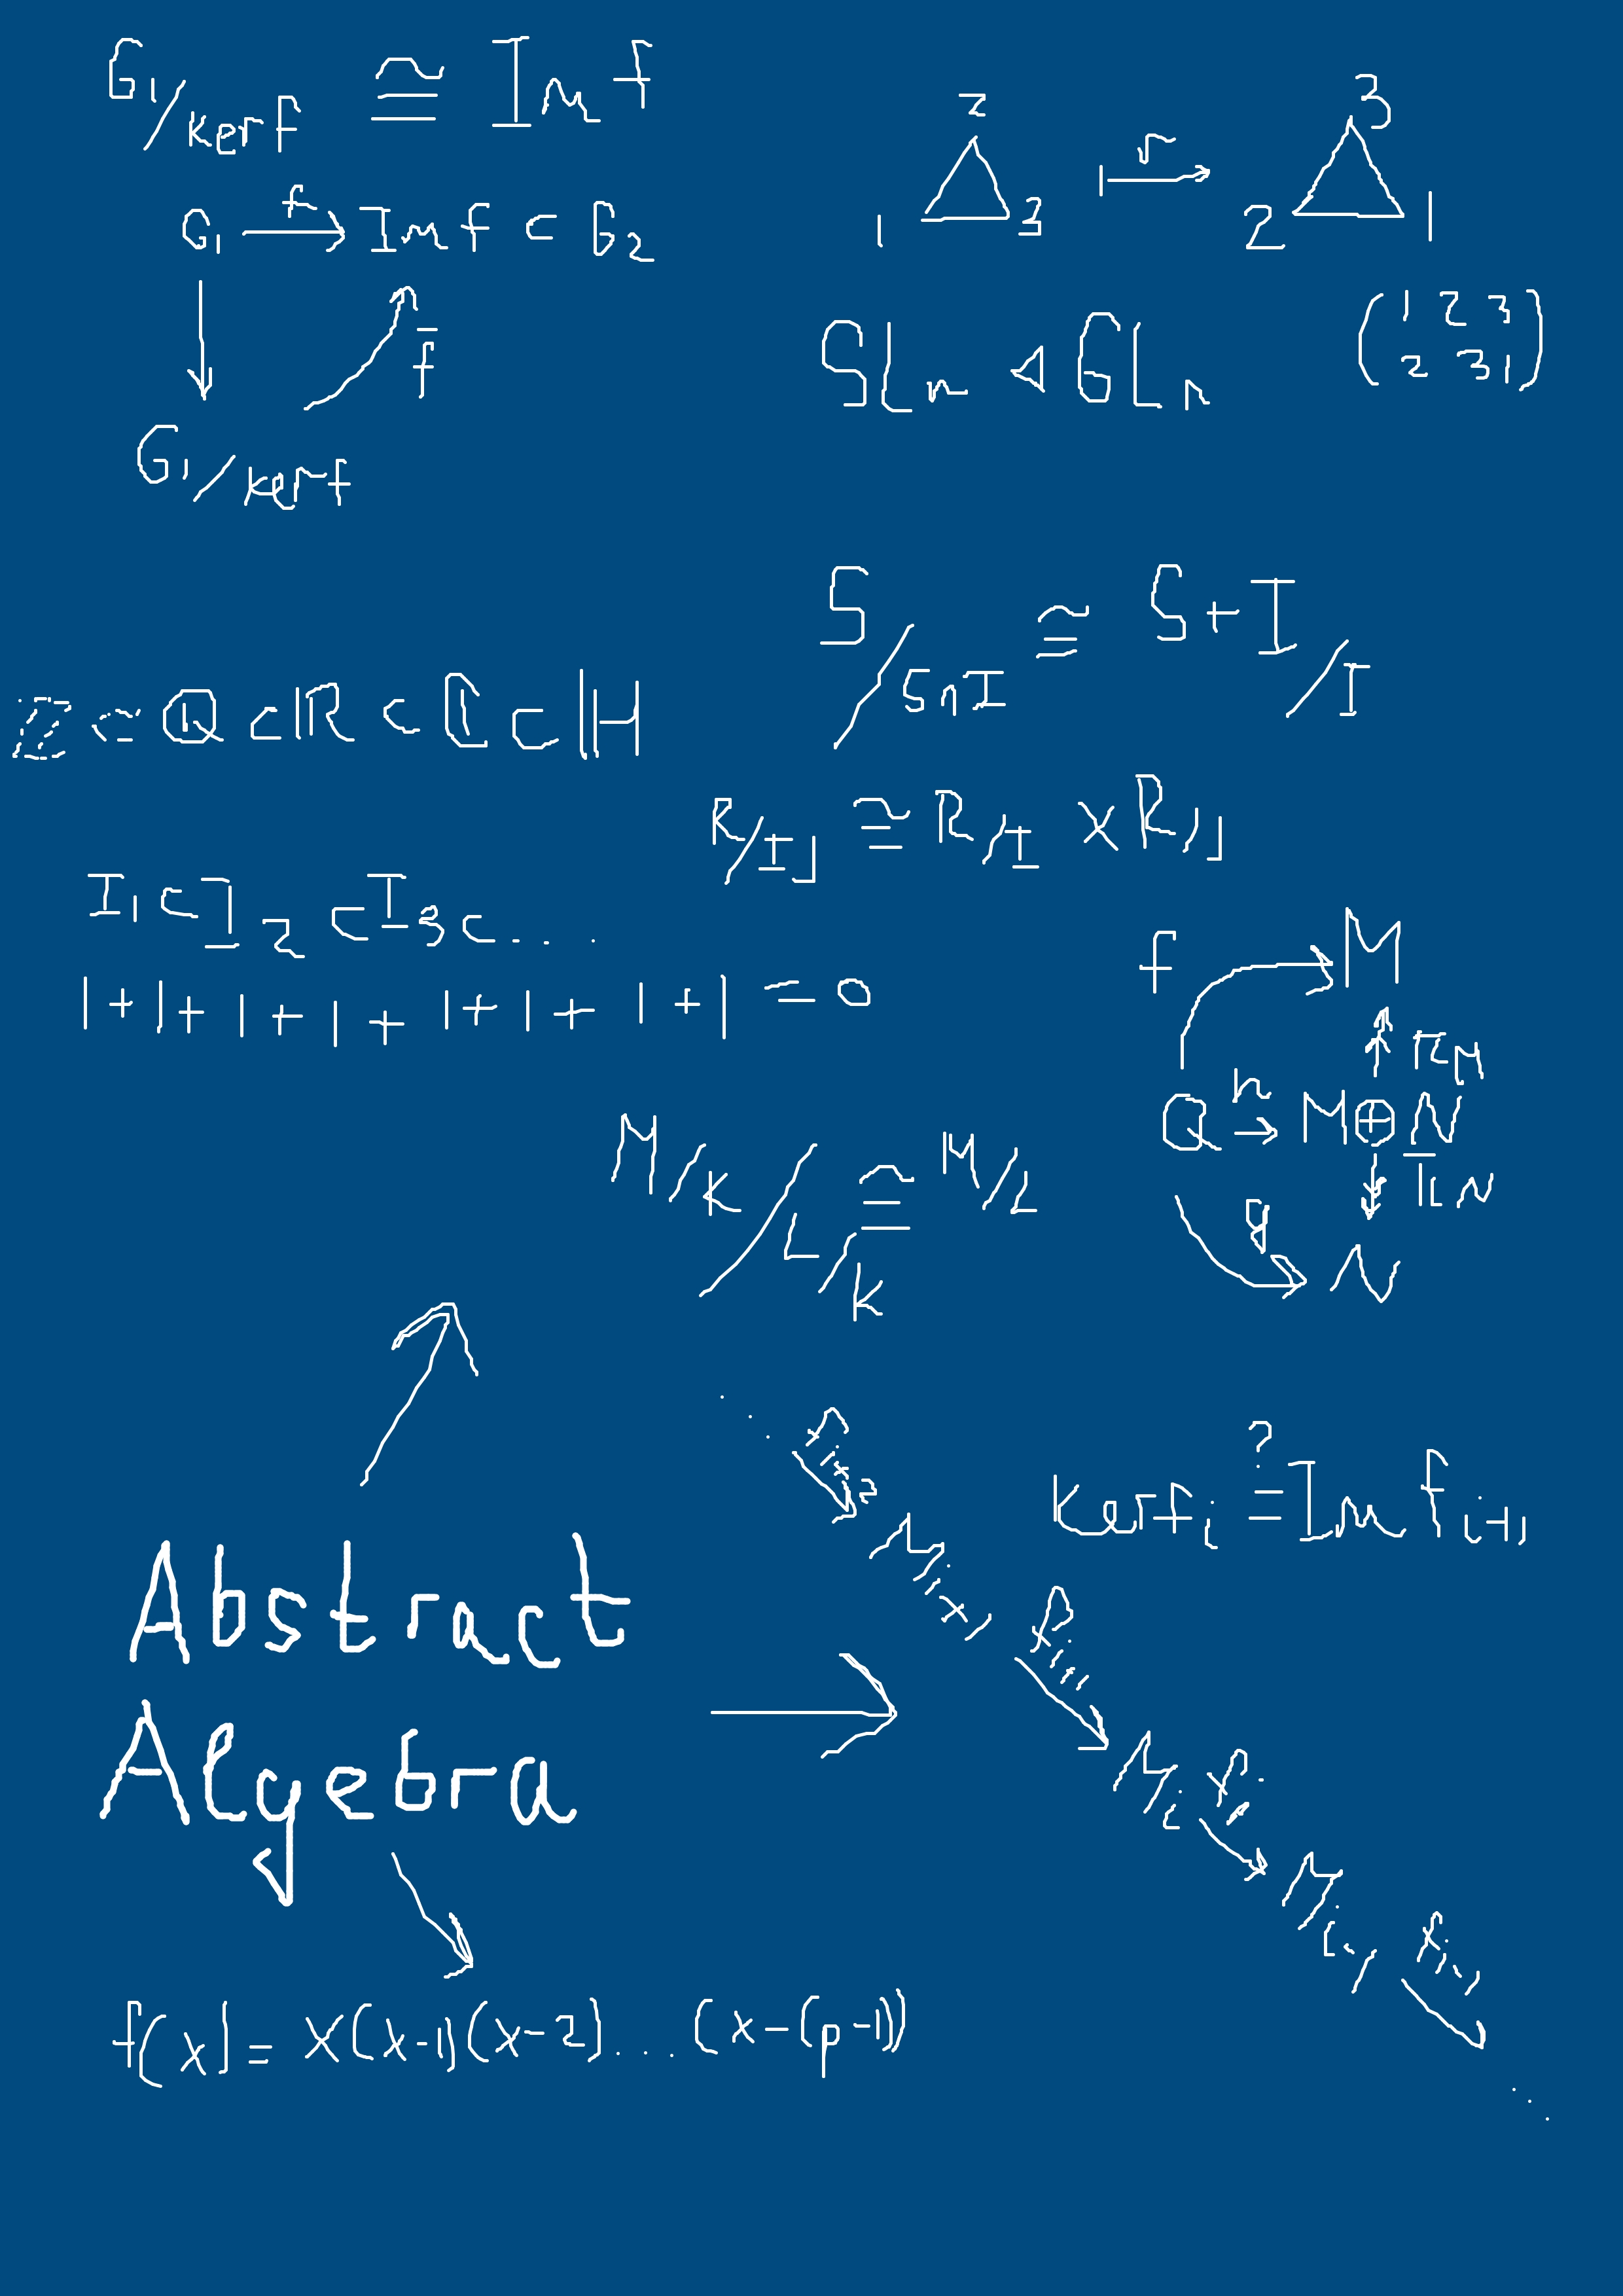
\includepdf{preview.jpg}
\tableofcontents
\newpage

\section{Кратні інтеграли}
\subsection{Кратні інтеграли по брусу}
\begin{definition}
\textbf{Прямокутним паралелепіпедом в} $\mathbb{R}^m$ або \textbf{$m$-вимірних брусом} називають множину
\begin{align*}
Q = [a_1,b_1] \times \dots \times [a_m,b_m]
\end{align*}
\textbf{Діаметром бруса} $Q$ називають число
\begin{align*}
d(Q) = \sup_{\vec{x},\vec{y} \in Q} \Norm{\vec{x}-\vec{y}}
\end{align*}
У нашому випадку $d(Q) = \sqrt{(b_1-a_1)^2 + \dots + (b_m-a_m)^2}$ - грубо кажучи, діагональ бруса.\\
\textbf{Об'ємом} або \textbf{мірою} бруса $Q$ називається додатне число
\begin{align*}
m(Q) = \prod_{k=1}^m (b_k-a_k)
\end{align*}
\end{definition}

\begin{figure}[H]
\centering
\begin{tikzpicture}
\fill[red] (0,0) rectangle (4,2);
\end{tikzpicture}
\caption*{Випадок $\mathbb{R}^2$ - прямокутник $Q = [0,4] \times [0,2]$ з діаметром $d(Q) = 2 \sqrt{5}$ та мірою $m(Q) = 4 \cdot 2 = 8$.}
\end{figure}

Далі нехай $Q = \displaystyle\prod_{k=1}^m [a_k,b_k]$ - брус. Ми розглянемо розбиття $\lambda_k = \{x_k^0, x_k^1,\dots,x_k^{n_k} \}$ відрізка $[a_k,b_k]$ для кожного $k = \overline{1,m}$. Нехай $\Delta x_k^v = x_k^{v+1} - x_k^v$, де $v = \overline{0,n_k-1}$.\\
Після такого розбиття ми отримаємо набір брусів $Q(v_1,\dots,v_m) = \displaystyle\prod_{k=1}^m [x_{k}^{v_k}, x_k^{v_k+1}]$, об'єм якого $m(Q(v_1,\dots,v_m)) = \displaystyle\prod_{k=1}^m \Delta x_k^{v_k}$.

\begin{figure}[H]
\centering
\begin{tikzpicture}
\fill[red] (0,0) rectangle (4,2);
\foreach \i in {1,2,3} {
	\draw (\i,0)--(\i,2);
	}
\foreach \i in {0.5,1.5} {
	\draw (0,\i)--(4,\i);
	}
\end{tikzpicture}
\caption*{Випадок $\mathbb{R}^2$ - відрізок $[0,4]$ має розбиття $\{0,1,2,3,4\}$ та відрізок $[0,2]$ має розбиття $\{0,0.5,1.5,2\}$. Після розбиття ми отримали набір прямокутників.}
\end{figure}

\begin{definition}
Цей набір брусів $\lambda = \{Q(v_1,\dots,v_m)\}$ називається \textbf{розбиттям бруса} $Q$.\\
\textbf{Діаметром розбиття} $\lambda$ називається число
\begin{align*}
|\lambda| = \max_{\substack{0 \leq v_k \leq n_k -1 \\ 1 \leq k \leq m}} d(Q(v_1,\dots,v_m))
\end{align*}
Грубо кажучи, шукаємо найбільшу діагональ бруса.
\end{definition}

\begin{remark}
$\displaystyle\sum_{\substack{0 \leq v_k \leq n_k -1 \\ 1 \leq k \leq m}} m(Q(v_1,\dots,v_m)) = m(Q)$.\\
Дійсно, зауважимо спочатку, що $\displaystyle\sum_{v=0}^{n_k-1} \Delta x_k^{v} = b_k-a_k$. А далі маємо:\\
$\displaystyle\sum_{\substack{0 \leq v_k \leq n_k-1 \\ 1 \leq k \leq m}} m(Q(v_1,\dots,v_m)) = \sum_{\substack{0 \leq v_k \leq n_k-1 \\ 1 \leq k \leq m}} \Delta x_1^{v_1} \dots \Delta x_m^{v_m} = \\ = \Delta x_1^0 \sum_{\substack{0 \leq v_k \leq n_k-1 \\ 2 \leq k \leq m}} \Delta x_2^{v_2} \dots \Delta x_m^{v_m} + \dots + \Delta x_1^{n_1-1} \sum_{\substack{0 \leq v_k \leq n_k-1 \\ 2 \leq k \leq m}} \Delta x_2^{v_2} \dots \Delta x_m^{v_m} = \\ = \sum_{\substack{0 \leq v_k \leq n_k-1 \\ 2 \leq k \leq m}} \Delta x_2^{v_2} \dots \Delta x_m^{v_m} (\Delta x_1^0 + \dots + \Delta x_1^{n_1-1}) = (b_1-a_1) \sum_{\substack{0 \leq v_k \leq n_k-1 \\ 2 \leq k \leq m}} \Delta x_2^{v_2} \dots \Delta x_m^{v_m} = \\
= \dots = (b_1-a_1)(b_2-a_2) \dots (b_m-a_m) = m(Q)$.
\end{remark}

\subsubsection*{Як отримати підрозбиття розбиття}
Маємо $Q$ - деякий брус та розбиття $\lambda$. Його ми отримали в результаті розбиття кожного відрізку.\\
Щоб отримати підрозбиття $\lambda'$ розбиття $\lambda$, ми запишемо підрозбиття $\lambda'_k$ розбиття кожного відрізка $\lambda_k$ (ми це робили додаванням точок).\\
\begin{figure}[H]
\centering
\begin{tikzpicture}
\fill[red] (0,0) rectangle (4,2);
\foreach \i in {1,2,3} {
	\draw (\i,0)--(\i,2);
	}
\foreach \i in {0.5,1.5} {
	\draw (0,\i)--(4,\i);
	}
\end{tikzpicture}
\qquad
\begin{tikzpicture}
\fill[red] (0,0) rectangle (4,2);
\foreach \i in {1,2,3} {
	\draw (\i,0)--(\i,2);
	}
\foreach \i in {0.5,1.5,2.5} {
	\draw[gray] (\i,0)--(\i,2);
	}
\foreach \i in {0.5,1.5} {
	\draw (0,\i)--(4,\i);
	}
\foreach \i in {1} {
	\draw[gray] (0,\i)--(4,\i);
	}
\end{tikzpicture}
\end{figure}
З'ясуємо, що буде відбуватись з кожним брусом $Q_1(v_1,\dots,v_m) = [x_k^{v_1},x_k^{v_1+1}] \times \dots \times [x_k^{v_m}, x_k^{v_m+1}]$.\\
І. Жодний відрізок, що бере участь в $Q(v_1,\dots,v_m)$, не підрозбивається. Тоді нічого з ним не буде.\\
II. Знайдеться відрізок, що бере участь в $Q(v_1,\dots,v_m)$, який підрозбивається. Не втрачаючи загальності, скажімо $[x_k^{v_1},x_k^{v_1+1}] = [x_k^{v_1}, y_0] \cup [y_0, y_1] \cup \dots \cup [y_p, x_k^{v_1+1}]$. У цьому випадку $y_0,y_1,\dots,y_p$ будуть точками, що були додані під час підзробиття відрізка. Тоді\\
$Q(v_1,\dots,v_m) = [x_k^{v_1},x_k^{v_1+1}] \times \dots \times [x_k^{v_m}, x_k^{v_m+1}] = \\
= ([x_k^{v_1}, y_0] \cup [y_0, y_1] \cup \dots \cup [y_p, x_k^{v_1+1}]) \times [x_k^{v_2}, x_k^{v_2+1}] \times \dots \times [x_k^{v_m}, x_k^{v_m+1}] = \\
= ([x_k^{v_1},y_0] \times [x_k^{v_2}, x_k^{v_2+1}] \times \dots \times [x_k^{v_m}, x_k^{v_m+1}]) \cup \dots \cup ([y_p,x_k^{v_k+1}] \times [x_k^{v_2}, x_k^{v_2+1}] \times \dots \times [x_k^{v_m}, x_k^{v_m+1}]) = \\
= Q_1 \cup \dots \cup Q_p$.\\
Ми тіпа розкриваємо дужки з точки зору теорії множин.\\
Таким чином, отримали, що брус розіб'ється на підбруси.\\
Причому згідно зі зауваженням вище, $\displaystyle\sum m(Q_i) = m(Q(v_1,\dots,v_m))$.\\
Саме за таким процесом, розбиваючи $\lambda$, отримаємо підрозбиття $\lambda'$.
\bigskip \\
Надалі вводиться позначення $\omega(\lambda) = \{ (v_1,\dots,v_m) | 0 \leq v_k \leq n_k-1, 1 \leq k \leq m \}$

\begin{definition}
Задано $Q$ - брус та функцію $f: Q \to \mathbb{R}$ - обмежена на $Q$ та $\lambda$ - розбиття бруса.\\
\textbf{Нижньою сумою Дарбу} для розбиття $\lambda$ та функції $f$ називається сума
\begin{align*}
L(f,\lambda) = \sum_{(v_1,\dots,v_m) \in \omega(\lambda)} \inf_{\vec{x} \in Q(v_1,\dots,v_m)} f(\vec{x}) \cdot m(Q(v_1,\dots,v_m))
\end{align*}
\textbf{Верхньою сумою Дарбу} для розбиття $\lambda$ та функції $f$ називається сума
\begin{align*}
U(f,\lambda) = \sum_{(v_1,\dots,v_m) \in \omega(\lambda)} \sup_{\vec{x} \in Q(v_1,\dots,v_m)} f(\vec{x}) \cdot m(Q(v_1,\dots,v_m))
\end{align*}
\end{definition}

\begin{definition}
Набір точок $\{ \vec{\xi}(v_1,\dots,v_m) | (v_1,\dots,v_m) \in \omega(\lambda) \} = \{ \vec{\xi} (v_1,\dots,v_m) \}$ назвемо \textbf{набором, що відповідає розбиттю} $\lambda$.\\
Тут $\vec{\xi}(v_1,\dots,v_m) \in Q(v_1,\dots,v_m)$.
\end{definition}

\begin{definition}
Задано $Q$ - брус та функцію $f: Q \to \mathbb{R}$ та $\lambda$ - розбиття бруса.\\
\textbf{Інтегральною сумою} для розбиття $\lambda$ з наборами $\{ \vec{\xi}(v_1,\dots,v_m) \}$ функції $f$ називається сума
\begin{align*}
\sigma(f,\lambda, \{ \vec{\xi}(v_1,\dots,v_m) \}) = \sum_{(v_1,\dots,v_m) \in \omega(\lambda)} f(\vec{\xi}(v_1,\dots,v_m)) \cdot m(Q(v_1,\dots,v_m))
\end{align*}
\end{definition}

%Fucking embarrassing
\iffalse
\begin{figure}[H]
\centering
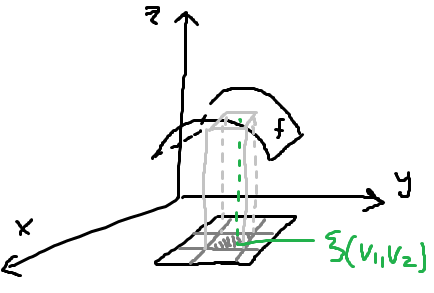
\includegraphics[scale=1]{RiemannSumR2.png}
\end{figure}
\fi

\begin{figure}[H]
\centering
\begin{tikzpicture}[scale = 1.4]
\draw[->] (0,0)--(4,0) node[anchor = north west] {$y$};
\draw[->] (0,0)--(0,3) node[anchor = south east] {$z$};
\draw[->] (0,0)--(-2.5,-2.5) node[anchor = north] {$x$};
\draw (1,-0.5)--(3,-0.5)--(2,-2)--(0,-2)--cycle;

\draw[dashed] (0,-2)--(0,-0.5);
\draw[dashed] (2,-2)--(2,0.5);
\draw[dashed] (3,-0.5)--(3,1);
\draw[dashed] (1,-0.5)--(1,2);

\filldraw [draw = red, fill = red!40] plot [smooth cycle] coordinates {(0,-0.5) (0.5,0.25) (1.2,0.5) (2,0.5) (2.3,0.8) (3,1) (2,1.8) (1,2) (0,1)} node[scale=1,red] at (0.2,0.2) {$f$};


%specific part of partition
\fill[blue!20] ({1/3+1},-1.5)--({2/3+1},-1)--({2/3+0.5},-1)--({1/3+0.5},-1.5)--cycle;

%draw a partition
\draw ({1/3},-1.5)--({1/3+2},-1.5);
\draw ({2/3},-1)--({2/3+2},-1);
\draw (0.5,-2)--(1.5,-0.5);
\draw (1,-2)--(2,-0.5);
\draw (1.5,-2)--(2.5,-0.5);

%go up to function
\fill[red] ({1/3+1-0.1},{-1.5+0.25}) circle (1pt);
\draw[red,dashed] ({1/3+1-0.1},{-1.5+0.25})--({1/3+1-0.1},0.9);
\fill[red] ({1/3+1-0.1},0.9) circle (1pt);

\draw[red,->] (-0.5,{-1.5+0.25})--({1/3+1-0.2},{-1.5+0.25}) node[scale=1,red] at (-0.6,{-1.5+0.25-0.2}) {$\xi(v_1,v_2)$};

%rectangle on surface
\draw[dashed] ({1/3+1},0.7)--({2/3+1},{0.7+0.5})--({2/3+0.5},{0.7+0.5})--({1/3+0.5},{0.7})--cycle;
\draw[dashed] ({1/3+1},-1.5)--({1/3+1},0.7);
\draw[dashed] ({2/3+1},-1)--({2/3+1},1.2);
\draw[dashed] ({2/3+0.5},-1)--({2/3+0.5},1.2);
\draw[dashed] ({1/3+0.5},-1.5)--({1/3+0.5},0.7);
\end{tikzpicture}
\end{figure}

\begin{definition}
Функція $f$ називається \textbf{інтегрованою за Ріманом}, якщо
\begin{align*}
\exists I \in \mathbb{R}: \forall \varepsilon > 0: \exists \delta(\varepsilon): \forall (\lambda, \vec{\xi}(v_1,\dots,v_m) ): |\lambda| < \delta \implies |\sigma(f,\lambda,\vec{\xi}(v_1,\dots,v_m)) - I| < \varepsilon
\end{align*}
Число $I$ називають \textbf{$m$-кратним інтегралом Рімана}.\\
Позначення: $\displaystyle\int\displaylimits_Q f(\vec{x})\,d\vec{x}$ \hspace{3cm} або $\displaystyle\int_{a_1}^{b_1} \dots \int_{a_m}^{b_m} f(x_1,\dots,x_m)\,dx_1\dots \,dx_m$
\end{definition}

\begin{example}
Довести, що $f(\vec{x}) = 1$ - інтегрована на брусі $Q$ та $\displaystyle\int\displaylimits_Q 1\,dx = m(Q)$.\\
Дійсно, $\displaystyle\sigma(f,\lambda,\{\vec{\xi}(v_1,\dots,v_m) \}) = \sum_{(v_1,\dots,v_m) \in \omega(\lambda)} m(Q(v_1,\dots,v_m)) = m(Q)$.\\
Отже, $\forall \varepsilon > 0: \exists \delta: \forall (\lambda, \{ \vec{\xi}(v_1,\dots,v_m \}): |\lambda| < \delta \implies |\sigma(f,\lambda,\{ \vec{\xi}(v_1,\dots,v_m) \} - m(Q)| = 0 < \varepsilon$.\\
Отже, $\displaystyle\int\displaylimits_Q 1\,dx = m(Q)$.
\end{example}

\begin{theorem}
Задано функцію $f: Q \to \mathbb{R}$ - інтегрована по брусу $Q$. Тоді $f$ - обмежена на $Q$.\\
\textit{Довденення аналогічне, як в матані $\mathbb{R}$.}
\end{theorem}

Всі властивості, які відомі про суму Дарбу, зберігаються тут. Я просто нагадаю.

\begin{remark}
$L(f,\lambda) \leq \sigma(f,\tau,\{ \vec{\xi}(v_1,\dots,x_m) \}) \leq U(f,\lambda)$.
\end{remark}

\begin{lemma}
Задано функцію $f: Q \to \mathbb{R}$ - обмежена на брусі та будь-яке розбиття $\lambda$. Тоді маємо:\\
$L(f,\lambda) = \displaystyle\inf_{\{ \vec{\xi}(v_1,\dots,x_m) \}} \sigma(f,\tau,\{ \vec{\xi}(v_1,\dots,x_m) \}) \hspace{1cm} U(f,\lambda) = \displaystyle\sup_{\{ \vec{\xi}(v_1,\dots,x_m) \}} \sigma(f,\tau,\{ \vec{\xi}(v_1,\dots,x_m) \})$
\end{lemma}

\begin{lemma}
Задано функцію $f: Q \to \mathbb{R}$ - обмежена на брусі та розбиття $\lambda$. Також задамо підрозбиття $\lambda'$. Тоді $U(f,\lambda) \geq U(f,\lambda')$, а також $L(f,\lambda) \leq L(f,\lambda')$.
\end{lemma}

\begin{lemma}
Задано функцію $f: Q \to \mathbb{R}$ - обмежена на брусі. Візьмемо будь-які два розбиття $\lambda', \lambda''$.\\
Тоді $L(f,\lambda') \leq U(f,\lambda'')$.
\end{lemma}

\begin{definition}
\textbf{Верхнім/нижнім інтегралом Дарбу} будемо називати такі вирази:
\begin{align*}
I^*(f) = \inf_\lambda U(f,\lambda) \hspace{1cm} I_*(f) = \sup_{\lambda} L(f,\lambda)
\end{align*}
\end{definition}

\begin{remark}
Справедлива така нерівність: $I_*(f) \leq I^*(f)$.
\end{remark}

\begin{theorem}[Перший критерій інтегрованості]
Задано функцію $f: Q \to \mathbb{R}$, де $Q$ - брус.\\
$f$ - інтегрована на $Q \iff f -$ обмежена на $Q$ та $I_*(f) = I^*(f)$.
\end{theorem}

\begin{theorem}[Другий критерій інтегрованості]
Задано функцію $f: Q \to \mathbb{R}$, де $Q$ - брус.\\
$f$ - інтегрована на $Q \iff f -$ обмежена на $Q$ та $\forall \varepsilon > 0: \exists \lambda: U(f,\lambda) - L(f,\lambda) < \varepsilon$.
\end{theorem}

\begin{theorem}
Задано функцію $f \in C(Q)$, де $Q$ - брус. Тоді $f$ - інтегрована на $Q$.\\
\textit{Доведення аналогічне, як в матані $\mathbb{R}$.}
\end{theorem}

\begin{theorem}
Задано $f: Q \to \mathbb{R}$, де $Q$ - брус. Припустимо, що $Q = Q_1 \cup Q_2$, де $Q_1,Q_2$ - бруси, що не мають спільних внутрішніх точок.\\
$f$ - інтегрована на $Q \iff f$ - інтегрована на $Q_1$ та $Q_2$.\\
\textit{Поки скіп.}
\end{theorem}

\subsection{Зведення кратних інтегралів до послідовних однократних}
Ми хочемо обчислити $\displaystyle\int\displaylimits_Q f(\vec{x})\,d\vec{x}$ через однократні інтеграли Рімана.\\
Маємо брус $Q \subset \mathbb{R}^m$. Розглянемо такі бруси:\\
$Q_k = \displaystyle\prod_{\substack{}1 \leq i \leq m \\ i \neq k} [a_i,b_i]$, де $Q_k \subset \mathbb{R}^{m-1}$. Даний брус - це проєкція брусу $Q$ на гіперплощину $x_k = 0$.\\
Припустимо, що $f \in C(Q)$. Тоді $\forall \leq 1 \leq k \leq m: \forall c \in [a_k,b_k]: f \in C(Q \cap \{ \vec{x} | x_k = c \}$.\\
Тому для кожного $x \in [a_k,b_k]$ визначається $(m-1)$-кратний інтеграл по $Q_k$:\\
$g_k(x) = \displaystyle\int\displaylimits_{Q_k}f(x_1,\dots,x_{k-1},x_k,x_{k+1},\dots,x_m)\,dx_1\dots \,dx_{k-1}\,dx_{k+1}\,\dots\,dx_m$.

\begin{lemma}
$g_k \in C([a_k,b_k])$.
\end{lemma}

\begin{proof}
$f \in C(Q)$, де $Q$ - компакт $\implies \forall \varepsilon > 0: \exists \delta: \forall \vec{x}, \vec{y}: \Norm{\vec{x} - \vec{y}} < \delta \implies |f(\vec{x}) - f(\vec{y})| < \dfrac{\varepsilon}{m(Q)}$.\\
Оберемо $x',x'' \in [a_k,b_k]$ так, щоб $|x'-x''|<\delta$. Тоді для векторів\\
$\vec{x'} = (x_1,\dots,x_{k-1},x',x_{k+1},\dots,x_m)$\\
$\vec{x''} = (x_1,\dots,x_{k-1},x'',x_{k+1},\dots,x_m)$,\\
де $(x_1,\dots,x_{k-1},x_{k+1},\dots,q_m) \in Q_k$, ми маємо:\\
$\Norm{\vec{x'} - \vec{x''}} = |x'-x''| < \delta$, а тому $|f(\vec{x'}) - f(\vec{x''})| < \dfrac{\varepsilon}{m(Q_k)}$.\\
$\displaystyle |g_k(x') - g_k(x'')| \leq \dfrac{\varepsilon}{m(Q_k)} \int\displaylimits_{Q_k} dx_1\dots dx_{k-1}\,dx_{k+1}\dots dx_m = \varepsilon$.\\
Таким чином, $g_k \in C_{unif}([a_k,b_k]) \implies g_k \in C([a_k,b_k])$.
\end{proof}

\begin{theorem}
$\displaystyle\int\displaylimits_Q f(\vec{x})\,d\vec{x} = \int_{a_k}^{b_k} \left( \int\displaylimits_{Q_k} f(x_1,\dots,x_{k-1},x_k,x_{k+1},\dots,x_m)\,dx_1\dots \,dx_{k-1}\,dx_{k+1}\,\dots\,dx_m \right)\,dx_k$
\end{theorem}

\begin{proof}
$f \in \mathcal{R}(Q)$, тому що ми вимагали функцію $f \in C(Q)$. Тому,\\
$\forall \varepsilon > 0: \exists \lambda: U(f,\lambda) - L(f,\lambda) < \varepsilon$.\\
Розбиття $\lambda$ природним чином розбиває брус $Q_k$. Маємо:\\
$\displaystyle\int_{a_k}^{b_k} g_k(x)\,dx = \sum_{v_k = 0}^{n_k-1} \int_{x_k(v_k)}^{x_k(v_k+1)}g_k(x)\,dx \leq \sum_{v_k=0}^{n_k-1} \sup_{x \in [x_k(v_k),x_k(v_k+1)]} g_k(x) \cdot \Delta x_k(v_k) \leq \\
\leq \sum_{v_k=0}^{n_k-1} \sup_{x \in [x_k(v_k),x_k(v_k+1)]} \left( \sum_{v_1,\dots,v_{k-1},v_{k+1},\dots,v_m} \sup_{\substack{(x_1,\dots,x_{k-1},x_{k+1},\dots,x_m) \\ \in \prod_{i \neq k} [x_i(v_i), x_i(v_i+1)]}} f(x_1,\dots,x_{k-1},x,x_{k+1},\dots,x_m) \prod_{i \neq k} \Delta x_i(v_i) \right) \Delta x_k(v_k) \\
\overset{?}{\leq} \sum_{v_k=0}^{n_k-1} \sum_{v_1,\dots,v_{k+1},\dots,v_m} \sup_{x \in [x_k(v_k), x_k(v_k+1)]} \sup_{\substack{(x_1,\dots,x_{k-1},x_{k+1},\dots,x_m) \\ \in \prod_{i \neq k} [x_i(v_i), x_i(v_i+1)]}} f(x_1,\dots,x_{k-1},x,x_{k+1},\dots,x_m) \prod_{i \neq k} \Delta x_i(v_i) \Delta x_k(v_k) \overset{??}{\leq} \\ \overset{??}{\leq} \sum_{v_1,\dots,v_m} \sup_{\vec{x} \in Q(v_1,\dots,v_m)} f(\vec{x}) m(Q(v_1,\dots,v_m)) = U(f,\lambda)$.\\
Пояснення до кількох нерівностей.\\
$\overset{?}{\leq}$. Поясню на функції двох змінних. У нас тут записано \\ $\displaystyle\sup_{y \in [y(v_2),y(v_2+1)]} \left( \sup_{x \in [x(0),x(1)]} f(x,y) + \dots + \sup_{x \in [x(n_1-1), x(n_1)] }f(x,y)\right)$.\\
Кожний $\displaystyle\sup_{x \in [x(v_1),x(v_1+1)]} f(x,y)$ стане функцією від однієї змінної (у цьому випвадку від $y$), всі вони будуть визначені на одному відрізку $[y(v_2),y(v_2+1)]$. А ми вже знаємо, що $\displaystyle\sup_D (f+g) \leq \sup_D f + \sup_D g$. Отже,\\
$\displaystyle\sup_{y \in [y(v_2),y(v_2+1)]} \left( \sup_{x \in [x(0),x(1)]} f(x,y) + \dots + \sup_{x \in [x(n_1-1), x(n_1)] }f(x,y)\right) \leq \\ \leq \sup_{y \in [y(v_2),y(v_2+1)]} \sup_{x \in [x(0),x(1)]} f(x,y) + \dots + \sup_{y \in [y(v_2),y(v_2+1)]} \sup_{x \in [x(n_1-1), x(n_1)]} f(x,y)$.\\
$\overset{??}{\leq}$. Поясню на функції двох змінних. Хочемо $\displaystyle\sup_{y \in [y(v_k),y(v_k+1)]} \sup_{x \in [x(v_l),x(v_l+1)]} f(x,y) \leq \sup_{\substack{x \in [x(v_l),x(v_l+1)] \\ y \in [y(v_k),y(v_k+1)]}} f(x,y)$.\\
Позначимо $\displaystyle\sup_{(x,y)} f(x,y) = M$. Тоді $\forall (x,y): f(x,y) \leq M$. Зокрема $\forall x: f(x,y) \leq M \\ \implies \displaystyle\sup_x f(x,y) \leq M$, ця нерівність виконана $\forall y$. Тому звідси $\displaystyle\sup_y \sup_x f(x,y) \leq M$.\\
Аналогічним чином ми доводимо, що $\displaystyle\int_{a_k}^{b_k} g_k(x)\,dx \geq L(f,\lambda)$.\\
Оскільки $L(f,\lambda) \leq \displaystyle\int\displaylimits_Q f(\vec{x})\,d \vec{x} \leq U(f,\lambda)$, то звідси\\
$\displaystyle\abs{\int\displaylimits_Q f(\vec{x})\,d \vec{x} - \int_{a_k}^{b_k} g_k(x)\,dx} \leq U(f,\lambda) - L(f,\lambda) < \varepsilon$.\\
Оскільки це виконано $\forall \varepsilon >0$, то довели рівність.
\end{proof}

\begin{corollary}
$\displaystyle\int\displaylimits_Q f(\vec{x})\,d\vec{x} = \int_{a_m}^{b_m} \dots \int_{a_2}^{b_2} \int_{a_1}^{b_1} f(x_1,x_2,\dots,x_m)\,dx_1\,dx_2 \dots dx_m$.
\end{corollary}

\begin{remark}
Можна зауважити, що порядок інтегрування може бути довільним, не обов'язково в такому порядку.
\end{remark}

\begin{corollary}
$\displaystyle\int\displaylimits_Q f(\vec{x})\,d\vec{x} = \int\displaylimits_{Q_k} \left( \int_{a_k}^{b_k} f(x_1,\dots,x_{k-1},x_k,x_{k+1},\dots,x_m)\,dx_k \right)\,dx_1 \dots dx_{k-1}\,dx_{k+1}\,\dots dx_m$.\\
\textit{Випливає з попереднього наслідка.}
\end{corollary}

\begin{corollary}
$\displaystyle\int\displaylimits_Q \departial{f}{x_k}(\vec{x})\,d\vec{x} = \displaystyle\int\displaylimits_{Q_k} f(x_1,\dots,x_{k-1},b_k,x_{k+1},\dots,x_m)\,dx_1\dots dx_{k-1}\,dx_{k+1}\dots dx_m - \\ - \int\displaylimits_{Q_k} f(x_1,\dots,x_{k-1},a_k,x_{k+1},\dots,x_m)\,dx_1\dots dx_{k-1}\,dx_{k+1}\dots dx_m$.\\
Це за умовою, що $\departial{f}{x_k} \in C(Q)$.\\
\textit{Випливає з попереднього наслідка та формули Ньютона-Лейбніца.}
\end{corollary}

\iffalse
\begin{remark}
Пояснення нерівності $\overset{?}{\leq}$ під час доведення наведу на просішому прикладі, на $\mathbb{R}^2$.\\
$U(f,\lambda) \geq \displaystyle\sum_{\substack{0 \leq v_1 \leq n_1-1 \\ 0 \leq v_2 \leq n_2-1}} \sup_{(x,y) \in Q(v_1,v_2)} f(x,y) \Delta x(v_1) \Delta y(v_2) = \sum_{v_2=0}^{n_2-1} \left( \sum_{v_1=0}^{n_1-1} \sup_{(x,y) \in Q(v_1,v_2)} f(x,y) \Delta x(v_1) \right) \Delta y(v_2)$
\end{remark}
\fi

\iffalse
\begin{remark}
Спершу зрозуміємо, що ми знаємо, коли $Q$ - брус та $Q = Q_1 \cup Q_2$, причому $Q_1,Q_2$ - бруси, що не мають спільних внутрішніх точок.\\
$\displaystyle\prod_{k=1}^m [a_k,b_k] = \prod_{k=1}^m [a_k^1,b_k^1] \cup \prod_{k=1}^m [a_k^2,b_k^2] = \prod_{k=1}^m ([a_k^1,b_k^1] \cup [a_k^2,b_k^2])$
\end{remark}

\begin{proof}
\rightproof Дано: $f$ - інтегрована на $Q$, тобто $\forall \varepsilon > 0: \exists \lambda: U(f,\lambda) - L(f,\lambda) < \varepsilon$.\\
Ми зараз створимо два нових розбиття: $\lambda_1$ для $Q_1$ та $\lambda_2$ для $Q_2$.\\
Для бруса $Q(v_1,\dots,v_m)$ із розбиття $\lambda$ є кілька сценаріїв:\\
$Q(v_1,\dots,v_m) \subset Q_1$, при цьому $Q(v_1,\dots,v_m) \cap Q_2$ має або спільні граничні точки, або порожню множину. Тоді $Q(v_1,\dots,v_m) \in \lambda_1$.\\
$Q(v_1,\dots,v_m) \subset Q_2$, при цьому $Q(v_1,\dots,v_m) \cap Q_1$ має або спільні граничні точки, або порожню множину. Тоді $Q(v_1,\dots,v_m) \in \lambda_2$.\\
$Q(v_1,\dots,v_m) \cap Q_1$ та $Q(v_1,\dots,v_m) \cap Q_2$ мають непорожній перетин, причому містять внутрішні точки $Q_1$ та $Q_2$. Тоді $Q(v_1,\dots,v_m)$ ми можемо розбити на $Q(v_1,\dots,v_m)^1, Q(v_1,\dots,v_m)^2$, щоб кожна з них лежала відповідно в $Q_1,Q_2$.
\end{proof}
\fi

\newpage

\section{Інтегрування по множинах}
Для власного спрощення розглядаю простір $\mathbb{R}^2$. Всі інші міркування можна скопіювати для $\mathbb{R}^m$.

Допоміжна теорема на майбутнє.
\begin{theorem}[Теорема Вейєрштрасса про наближення неперервної функції]
Задано $f \in C([a,b])$. Тоді $\forall \varepsilon > 0: \exists P_\varepsilon$ - многочлен: $\forall x \in [a,b]: |f(x) - P_\varepsilon(x)| < \varepsilon$.
\end{theorem}

\begin{proof}
Розглянемо випадок, коли функція $f \in C([0,1])$. Введемо такий многочлен:\\
$B_n(f,x) = \displaystyle\sum_{k=0}^n f \left( \dfrac{k}{n} \right) p_{nk}(x)$, де $p_{nk}(x) = C_n^k x^k (1-x)^{n-k}$.\\
Тут $n \in \mathbb{N}, x \in [0,1]$. Її ще називають \textbf{многочленом Бернштейна}. \\
(щось схожий на сумування ймовірностей за схемою Бернуллі).\\
Тут вважаємо, що $0^0 = 1$, бо можна довизначити усунені точки.\\
За теоремою Кантора, для числа $\dfrac{\varepsilon}{2}$\\
$\exists \delta: \forall x_1,x_2 \in [0,1]: |x_1-x_2| < \delta \implies |f(x_1)-f(x_2)| < \dfrac{\varepsilon}{2}$.\\
Зауважимо, що $\displaystyle\sum_{k=0}^n p_{nk}(x) = 1$.
Тоді\\
$|f(x) - B_{n}(f,x)| = \displaystyle\abs{\sum_{k=0}^n \left( f(x) - f\left( \dfrac{k}{n} \right) \right) p_{nk}(x) } \leq \sum_{k=0}^n \abs{f(x) - f\left( \dfrac{k}{n} \right)} |p_{nk}(x)| \\
= \sum_{k: \left| x -\frac{k}{n} \right| < \delta} \abs{f(x) - f\left( \dfrac{k}{n} \right)} p_{nk}(x) + \sum_{k: \left| x -\frac{k}{n} \right| \geq \delta} \abs{f(x) - f\left( \dfrac{k}{n} \right)} p_{nk}(x) \boxed{<}$\\
У першій сумі $\abs{f(x) - f\left( \dfrac{k}{n} \right)} < \dfrac{\varepsilon}{2}$ за Кантором.\\
У другій сумі $\abs{f(x) - f\left( \dfrac{k}{n} \right)} \leq 2C$, оскільки $f$ - обмежена.\\
$\boxed{<} \displaystyle \dfrac{\varepsilon}{2} \sum_{k: \left| x -\frac{k}{n} \right| < \delta} p_{nk}(x) + 2C \sum_{k: \left| x -\frac{k}{n} \right| \geq \delta} p_{nk}(x) \overset{?}{\leq} \dfrac{\varepsilon}{2} \sum_{k=0}^n p_{nk}(x) + 2C \dfrac{1}{\delta^2} \sum_{k=0}^n \left( x -\dfrac{k}{n} \right)^2 p_{nk}(x) = \dfrac{\varepsilon}{2} + \dfrac{2C}{\delta^2} \dfrac{x(1-x)}{n} \leq \dfrac{\varepsilon}{2} + \dfrac{C}{2n\delta^2}$\\
Пояснення $\overset{?}{\leq}$. Маємо $\abs{x - \dfrac{k}{n}} \geq \delta \implies \left( x - \dfrac{k}{n} \right)^2 \geq \delta^2 \implies \dfrac{1}{\delta^2} \left( x - \dfrac{k}{n} \right)^2 \geq 1$. А отже, звідси\\
$\displaystyle\sum_{k: \abs{x - \frac{k}{n}} \geq \delta} p_{nk}(x) \cdot 1 \leq \sum_{k: \abs{x - \frac{k}{n}} \geq \delta} p_{nk}(x) \dfrac{1}{\delta^2} \left( x - \dfrac{k}{n} \right)^2 \leq \dfrac{1}{\delta^2} \sum_{k=0}^n p_{nk}(x) \left( x - \dfrac{k}{n} \right)^2$.\\
Оскільки $\dfrac{C}{2n\delta^2} \to 0$, то $\exists N: \dfrac{C}{2n\delta^2} < \dfrac{\varepsilon}{2}$.\\
Таким чином, $\forall \varepsilon > 0: \exists N: \exists P_\varepsilon(x) = B_n(f,x): \forall x \in [0,1]: \\ |f(x)- P_{\varepsilon}(x)| < \varepsilon$.
\bigskip \\
У випадку $f \in C([a,b])$ ми розглянемо функцію $g(t) = f(a+t(b-a)) \in C([0,1])$.
\end{proof}

\begin{theorem}[Теорема Вейєрштрасса про наближення неперервної функції в $\mathbb{R}^n$]
Задано функцію $f \in C(A)$, де $A$ - компакт. Тоді $\forall \varepsilon > 0: \exists P_\varepsilon$ - многочлен: $\forall \vec{x} \in A: |f(\vec{x}) - P_\varepsilon(\vec{x})| < \varepsilon$.
\end{theorem}

\begin{proof}
У принципі, ідея та сама, що було зверху, просто трошки треба модифікувати.\\
Розглянемо випадок, коли функція $f \in C([0,1]^m)$, введемо такий многочлен:\\
$B_n(f,x_1,\dots,x_m) = \displaystyle\sum_{i_1=0}^{s_1} \dots \sum_{i_m=0}^{s_m} f\left( \dfrac{i_1}{s_1},\dots,\dfrac{i_m}{s_m} \right) p_{s_1 i_1}(x_1) \dots p_{s_m i_m}(x_m)$.\\
Тут $n \in \mathbb{N}$, а також $p_{s_j i_j}(x_j) = C_{s_j}^{i_j} x_j^{i_j}(1-x_j)^{s_j-i_j}$. Тут аналогічно $\displaystyle\sum_{i_j=0}^{s_j} p_{s_ji_j}(x_j) = 1$. Всюди $j = \overline{1,m}$.\\
Тоді також $\displaystyle\sum_{i_1=0}^{s_1} \dots \sum_{i_m=0}^{s_m} p_{s_1i_1}(x_1) \dots p_{s_m i_m}(x_m) = \sum_{i_1=0}^{s_1} p_{s_1i_1}(x_1) \dots \sum_{i_m = 0}^{s_m} p_{s_m i_m}(x_m) = 1$.\\
Аналогічно функцію $f$ можна довизначити всюди там, де $0^0$ відбувається. Власне,\\
$|f(x) - B_n(f,x_1,\dots,x_m)|$ оцінюється буквально так само, як це було. Будуть хіба що пару нюансів: ми ділимо суму на: \\
I. $(i_1,\dots,i_m)$, щоб $\Norm{(x_1,\dots,x_m) - \left(\dfrac{i_1}{s_1},\dots,\dfrac{i_m}{s_m} \right)} < \delta$\\
II. $(i_1,\dots,i_m)$, щоб $\Norm{(x_1,\dots,x_m) - \left(\dfrac{i_1}{s_1},\dots,\dfrac{i_m}{s_m} \right)} \geq \delta$\\
Із другого випливає, що $\left( x_1 - \dfrac{i_1}{s_1}\right)^2 + \dots + \left( x_m - \dfrac{i_m}{s_m} \right)^2 \geq \delta^2$, а звідси\\
$1 \leq \dfrac{1}{\delta^2} \left( x_1 - \dfrac{i_1}{s_1}\right)^2 + \dots + \dfrac{1}{\delta^2} \left( x_m - \dfrac{i_m}{s_m}\right)^2$. Ну а там вже аналогічно доведеться все, що треба. Але це тільки частинний випадок.\\
Тепер нехай $f \in C(A)$, де $A$ - компакт. Звідси обмеженість множини, а тому $\exists R > 0: A \subset U_R(\vec{0})$.\\
Навколо цього окола можемо описати куб $S_R = \{ \vec{x} \in \mathbb{R}^m: |x_1| \leq R, \dots |x_m| \leq R \} \supset U_R(\vec{0})$.\\
Ми продовжимо функцію $f$ до $S_R$ так, щоб $f \in C(S_R)$. Це можна зробити, завдяки теоремі Тітце.\\
Зауважимо, що $S_R = [-x_1,x_1] \times \dots \times [-x_m,x_m]$. А ось тепер розглянемо функцію $g(t_1,\dots,t_m) = f(-x_1+2t_1x_1, \dots, -x_m+2t_mx_m)$, причому тепер $t_1,\dots,t_m \in [0,1]$. Для цієї функції вже многочлен існує, за попереднім пунктом.
\end{proof}

\subsection{Розбиття простору $\mathbb{R}^2$}
\begin{definition}
\textbf{Розбиття нульового порядку} простора $\mathbb{R}^2$ визначається ось так:
\begin{align*}
\mathbb{R}^2 = \bigcup_{n_1,n_2 \in \mathbb{Z}} Q^{(0)}(n_1,n_2), \\
Q^{(0)}(n_1,n_2) = [n_1,n_1+1] \times [n_2,n_2+1]
\end{align*}
\iffalse
Q^{(0)}(n_1,n_2) = \{ (x,y): x \in [n_1,n_1+1], \hspace{0.5cm} y \in [n_2,n_2+1]\} \\
\fi
Тобто ми $\mathbb{R}^2$ розбиваємо на квадрати зі сторонами $1$ таким чином, щоб координати вершин були цілими числами.
\end{definition}

\begin{figure}[H]
\centering
\begin{tikzpicture}
\draw[->] (-2.5,0)--(2.5,0) node[anchor = north west] {$x$};
\draw[->] (0,-2.5)--(0,2.5) node[anchor = south east] {$y$};
\node at (1.1,-0.2) {$1$};
\node at (0.1,-0.2) {$0$};
\node at (-0.2,0.9) {$1$};
\foreach \i in {-2,-1,1,2} {
\draw (-2,\i)--(2,\i);
}
\foreach \i in {-2,-1,1,2} {
\draw (\i,-2)--(\i,2);
}
\end{tikzpicture}
\end{figure}

\begin{definition}
\textbf{Розбиття першого порядку} простора $\mathbb{R}^2$ визначається ось таке саме об'єднання, але тепер об'єднання з $Q^{(1)}(n_1,n_2)$, де
\begin{align*}
Q^{(1)}(n_1,n_2) = \left[ \dfrac{n_1}{2}, \dfrac{n_1+1}{2} \right] \times \left[ \dfrac{n_2}{2}, \dfrac{n_2+1}{2} \right]
\iffalse Q^{(1)} = \left\{ (x,y): x \in \left[\dfrac{n_1}{2},\dfrac{n_1+1}{2} \right], \hspace{0.5cm} y \in \left[\dfrac{n_2}{2},\dfrac{n_2+1}{2} \right] \right\}
\fi
\end{align*}
Тобто ми $\mathbb{R}^2$ розбиваємо на квадрати зі сторонами $\dfrac{1}{2}$ так, щоб вершини були кратними до $\dfrac{1}{2}$.
\end{definition}

\begin{figure}[H]
\centering
\begin{tikzpicture}
\draw[->] (-2.5,0)--(2.5,0) node[anchor = north west] {$x$};
\draw[->] (0,-2.5)--(0,2.5) node[anchor = south east] {$y$};
\node at (1.1,-0.2) {$1$};
\node at (0.1,-0.2) {$0$};
\node at (-0.2,0.9) {$1$};
\foreach \i in {-2,-1.5,-1,-0.5,0.5,1,1.5,2} {
\draw (-2,\i)--(2,\i);
}
\foreach \i in {-2,-1.5,-1,-0.5,0.5,1,1.5,2} {
\draw (\i,-2)--(\i,2);
}
\end{tikzpicture}
\end{figure}

На даному етапі можна зауважити, що $Q^{(1)}(n_1,n_2)$ можна отримати від $Q^{(0)}(k_1,k_2)$ шляхом ділення відрізків навпіл. Дійсно,\\
$Q^{(0)}(k_1,k_2) = [k_1,k_1+1] \times [k_2,k_2+1] = \\ = \left(\left[ \dfrac{2k_1}{2}, \dfrac{2k_1+1}{2} \right] \cup \left[ \dfrac{2k_1+1}{2}, \dfrac{2k_1+2}{2} \right]\right) \times \left(\left[ \dfrac{2k_2}{2}, \dfrac{2k_2+1}{2} \right] \cup \left[ \dfrac{2k_2+1}{2}, \dfrac{2k_2+2}{2} \right]\right) = \\
= Q^{(1)}\left( 2k_1, 2k_2 \right) \cup Q^{(1)}\left( 2k_1+1, 2k_2 \right) \cup Q^{(1)}\left( 2k_1, 2k_2+1 \right) \cup Q^{(1)}\left( 2k_1+1, 2k_2+1 \right)$.\\
Таким чином, утвориться $2^{\textcolor{red}{2}} = 4$ брусів $Q^{(1)}$. Степінь $\textcolor{red}{2}$ -- розмірність простору. При вищій розмірності була б інша кількість брусів (думаю, зрозуміло яка).

\begin{definition}
\textbf{Розбиття $n$-го порядку} простора $\mathbb{R}^2$ визначається ось таке саме об'єднання, але тепер об'єднання з $Q^{(n)}(n_1,n_2)$, де
\begin{align*}
Q^{(n)}(n_1,n_2) = \left[ \dfrac{n_1}{2^n}, \dfrac{n_1+1}{2^n} \right] \times \left[ \dfrac{n_2}{2^n}, \dfrac{n_2+1}{2^n} \right]
\iffalse
Q^{(n)} = \left\{ (x,y): x \in \left[\dfrac{n_1}{2^n},\dfrac{n_1+1}{2^n} \right], \hspace{0.5cm} y \in \left[\dfrac{n_2}{2^n},\dfrac{n_2+1}{2^n} \right] \right\}
\fi
\end{align*}
\end{definition}

\begin{remark}
Важливі спостереження щодо цих брусів. Червоним написана розмірність простору:
\begin{enumerate}[nosep,wide=0pt,label={\arabic*)}]
\item $d\left(Q^{(n)}(n_1,n_2)\right) = \sqrt{\textcolor{red}{2}} \cdot 2^{-n}$;
\item $m\left(Q^{(n)}(n_1,n_2)\right) = \left( \dfrac{1}{2^n} \right)^{\textcolor{red}{2}}$;
\item $Q^{(n)}(n_1,n_2)$ та $Q^{(n)}(k_1,k_2)$, які різні, тобто $(n_1,n_2) \neq (k_1,k_2)$, можуть перетинатися між собою, проте ніколи не мають спільних внутрішніх точок, тото $\Int \left( Q^{(n)}(n_1,n_2) \right) \cap \Int \left( Q^{(n)}(k_1,k_2) \right) = \emptyset$;
\item Задамо деяку обмежену множину $F \subset \mathbb{R}^2$. Тоді для будь-якого порядку розбиття $\mathbb{R}^2$ набір утворених брусів, що мають хоча б одну спільну точку з $F$, скінченний.
\end{enumerate}
\end{remark}

Позначення: $\pi^{(n)} = \{ Q^{(n)}(n_1,n_2) \mid n_1,n_2 \in \mathbb{Z}\}$ -- множина цих брусів довжиною $\dfrac{1}{2^n}$.

\subsection{Вимірні множини. Міра Жордана}
Уже відомо, що для бруса $Q = [a_1,b_1] \times [a_2,b_2]$ міра визначається як
\begin{align*} 
m(Q) = (b_1-a_1)(b_2-a_2).
\end{align*}
Нехай $G \subset \mathbb{R}^2$, яка допускає розклад в різні бруси $Q_i \in \pi^{(n)}$ при деякому $n$, тобто $G = \displaystyle\bigcup_{i=1}^s Q_i$. Тоді природно визначити \textbf{міру множини} $G$ ось так:
\begin{align*}
m(G) = \sum_{i=1}^s m(Q_i)
\end{align*}

\begin{remark}
Розклад $G$ не є єдиним, як можна побачити нижче. Тим не менш, значення міри не буде залежати від розбиття, тобто міра коректно визначена.
\end{remark}
\iffalse
\begin{figure}[H]
\centering
\begin{tikzpicture}
\fill[black!20] (0,0) rectangle (1,1);
\fill[black!40] (1,0.5) rectangle (2,2);
\fill[black!60] (1,0) rectangle (2.5,0.5);
\fill[black!20] (2.5,-1) rectangle (3.5,0.5);
\fill[black!40] (1.5,-1) rectangle (2.5,0);
\draw (0,0)--(0,1)--(1,1)--(1,2)--(2,2)--(2,0.5)--(3.5,0.5)--(3.5,-1)--(1.5,-1)--(1.5,0)--cycle node[anchor = east] {$G$};
\end{tikzpicture}
\qquad
\begin{tikzpicture}
\fill[black!20] (0,0) rectangle (1,1);
\fill[black!40] (1,1) rectangle (2,2);
\fill[black!60] (1,0) rectangle (2,1);
\fill[black!80] (2,0) rectangle (2.5,0.5);
\fill[black!20] (2.5,-1) rectangle (3.5,0.5);
\fill[black!40] (1.5,-1) rectangle (2.5,0);
\draw (0,0)--(0,1)--(1,1)--(1,2)--(2,2)--(2,0.5)--(3.5,0.5)--(3.5,-1)--(1.5,-1)--(1.5,0)--cycle node[anchor = east] {$G$};
\end{tikzpicture}
\end{figure}
\fi
\begin{figure}[H]
\centering
\begin{tikzpicture}
\fill[black!20] (0,0) rectangle (1,1);
\fill[black!20] (1,1) rectangle (2,2);
\fill[black!40] (1,0) rectangle (2,1);
\fill[black!20] (1,0) rectangle (2,-1);
\fill[black!40] (2,0) rectangle (3,-1);
\draw (0,0)--(0,1)--(1,1)--(1,2)--(2,2)--(2,0)--(3,0)--(3,-1)--(1,-1)--(1,0)--cycle;
\end{tikzpicture}
\qquad
\begin{tikzpicture}
\fill[black!20] (0,0) rectangle (1,1);
\fill[black!40] (0,0) rectangle (0.5,0.5);
\fill[black!40] (0.5,0.5) rectangle (1,1);
\fill[black!20] (1,1) rectangle (2,2);
\fill[black!40] (1,1) rectangle (1.5,1.5);
\fill[black!40] (1.5,1.5) rectangle (2,2);
\fill[black!20] (1,0) rectangle (2,1);
\fill[black!40] (1,0) rectangle (1.5,0.5);
\fill[black!40] (1.5,0.5) rectangle (2,1);
\fill[black!20] (1,0) rectangle (2,-1);
\fill[black!40] (2,0) rectangle (1.5,-0.5);
\fill[black!40] (1,-0.5) rectangle (1.5,-1);
\fill[black!20] (2,0) rectangle (3,-1);
\fill[black!40] (2.5,0) rectangle (3,-0.5);
\fill[black!40] (2,-0.5) rectangle (2.5,-1);
\draw (0,0)--(0,1)--(1,1)--(1,2)--(2,2)--(2,0)--(3,0)--(3,-1)--(1,-1)--(1,0)--cycle;
\end{tikzpicture}
\caption*{Одна й та сама фігура $G$, тільки одна з $\pi^{(n)}$, друга з $\pi^{(m)}$, причому $m > n$.}
\end{figure}

Насправді, ми вже пам'ятаємо, що кожний брус з $\pi^{(n)}$ можна розбити на об'єднання підбрусів з $\pi^{(m)}, m > n$. Тоді (також відомо) міра одного бруса дорівнює сумі мір підбрусів.
\bigskip \\
Нехай тепер $F \subset \mathbb{R}^2$ -- деяка обмежена множина. Визначимо ось такі множини для кожного $n \geq 0$:
\begin{align*}
F_{(n)} = \bigcup_{\substack{Q \in \pi^{(n)} \\ Q \subset F}} Q \qquad\qquad
F^{(n)} = \bigcup_{\substack{Q \in \pi^{(n)} \\ Q \cap F \neq \emptyset}} Q \qquad\qquad
\Delta F_{(n)} = \bigcup_{\substack{Q \not\subset F_{(n)} \\ Q \subset F^{(n)}}} Q
\end{align*}
\begin{figure}[H]
\centering
\begin{tikzpicture}
\begin{scope}[transparency group]
\begin{scope}[blend mode=multiply]
\fill[blue!50] (0,0) rectangle (3,0.5);
\fill[blue!50] (0.5,0.5) rectangle (3,1);
\fill[blue!50] (0.5,1) rectangle (2,1.5);
\draw[step=.5cm] (-0.4,-0.9) grid (3.9,2.4);
\fill [red!50, thick] plot [smooth cycle] coordinates {(0,0) (1,2) (3,1) (3,0)};

\node[red] at (0.25,0.25) {$F$};
\node[blue] at (2,-1.5) {$F_{(n)}$};
\end{scope}
\end{scope}
\end{tikzpicture}
\qquad
\begin{tikzpicture}
\begin{scope}[transparency group]
\begin{scope}[blend mode=multiply]
\fill[blue!50] (0,-0.5) rectangle (3,0);
\fill[blue!50] (-0.4,0) rectangle (3.5,0.5);
\fill[blue!50] (0,0.5) rectangle (3.5,1);
\fill[blue!50] (0,1) rectangle (3,1.5);
\fill[blue!50] (0.5,1.5) rectangle (2.5,2);
\draw[step=.5cm] (-0.4,-0.9) grid (3.9,2.4);
\fill [red!50, thick] plot [smooth cycle] coordinates {(0,0) (1,2) (3,1) (3,0)};

\node[red] at (0.25,0.25) {$F$};
\node[blue] at (2,-1.55) {$F^{(n)}$};
\end{scope}
\end{scope}
\end{tikzpicture}
\qquad
\begin{tikzpicture}
\begin{scope}[transparency group]
\begin{scope}[blend mode=multiply]
\fill[blue!50] (0,-0.5) rectangle (3,0);
\fill[blue!50] (-0.4,0) rectangle (0,0.5);
\fill[blue!50] (3,0) rectangle (3.5,0.5);
\fill[blue!50] (0,0.5) rectangle (0.5,1);
\fill[blue!50] (3,0.5) rectangle (3.5,1);
\fill[blue!50] (0,1) rectangle (0.5,1.5);
\fill[blue!50] (2,1) rectangle (3,1.5);
\fill[blue!50] (0.5,1.5) rectangle (2.5,2);
\draw[step=.5cm] (-0.4,-0.9) grid (3.9,2.4);
\fill [red!50, thick] plot [smooth cycle] coordinates {(0,0) (1,2) (3,1) (3,0)};

\node[red] at (0.25,0.25) {$F$};
\node[blue] at (2,-1.55) {$\Delta F_{(n)}$};
\end{scope}
\end{scope}
\end{tikzpicture}
\caption*{Тут червона область заповнена всередині, не просто множиина лінія.}
\end{figure}

\begin{remark}
У цьому випадку $\Delta F_{(n)} \neq F^{(n)} \setminus F_{(n)}$, тому що можна загубити граничні точки (фактично кажучи, границі множини).
\end{remark}

\begin{figure}[H]
\centering
\begin{tikzpicture}
\begin{scope}[transparency group]
\begin{scope}[blend mode=multiply]
\fill[blue!50] (0,-0.5) rectangle (3,0);
\fill[blue!50] (-0.4,0) rectangle (0,0.5);
\fill[blue!50] (3,0) rectangle (3.5,0.5);
\fill[blue!50] (0,0.5) rectangle (0.5,1);
\fill[blue!50] (3,0.5) rectangle (3.5,1);
\fill[blue!50] (0,1) rectangle (0.5,1.5);
\fill[blue!50] (2,1) rectangle (3,1.5);
\fill[blue!50] (0.5,1.5) rectangle (2.5,2);
%\draw[step=.5cm] (-0.4,-0.9) grid (3.9,2.4);
\fill[red!50, thick] plot [smooth cycle] coordinates {(0,0) (1,2) (3,1) (3,0)};

\node[red] at (0.25,0.25) {$F$};
\node[blue] at (2,-1.55) {$\Delta F_{(n)}$};
\end{scope}
\end{scope}
\end{tikzpicture}
\qquad
\begin{tikzpicture}
\begin{scope}[transparency group]
\begin{scope}[blend mode=multiply]
\fill[blue!50] (0,-0.5) rectangle (3,0);
\fill[blue!50] (-0.4,0) rectangle (0,0.5);
\fill[blue!50] (3,0) rectangle (3.5,0.5);
\fill[blue!50] (0,0.5) rectangle (0.5,1);
\fill[blue!50] (3,0.5) rectangle (3.5,1);
\fill[blue!50] (0,1) rectangle (0.5,1.5);
\fill[blue!50] (2,1) rectangle (3,1.5);
\fill[blue!50] (0.5,1.5) rectangle (2.5,2);

\draw[dashed] (3,0)--(0,0)--(0,0.5)--(0.5,0.5)--(0.5,1.5);
\draw[dashed] (0.5,1.5)--(2,1.5)--(2,1)--(3,1)--(3,0);

%\draw[step=.5cm] (-0.4,-0.9) grid (3.9,2.4);
\fill [red!50, thick] plot [smooth cycle] coordinates {(0,0) (1,2) (3,1) (3,0)};

\node[red] at (0.25,0.25) {$F$};
\node[blue] at (2,-1.55) {$F^{(n)} \setminus F_{(n)}$};
\end{scope}
\end{scope}
\end{tikzpicture}
\end{figure}

\begin{remark}
Якщо не існує бруса $Q \in \pi^{(n)}$, для якого $Q \subset F$, вважаємо, що $F_{(n)} = \emptyset$.
\end{remark}

\begin{figure}[H]
\centering
\begin{tikzpicture}
%\fill[blue!50] (0,0) rectangle (3,0.5);
%\fill[blue!50] (0.5,0.5) rectangle (3,1);
%\fill[blue!50] (0.5,1) rectangle (2,1.5);
\draw[step=.5cm] (-0.4,-0.9) grid (3.9,2.4);
\draw [red, thick] plot [smooth cycle] coordinates {(0,0) (1,2) (3,1) (3,0)};

\node[red] at (0.25,0.25) {$F$};
\node[blue] at (2,-1.5) {$F_{(n)} = \emptyset$};
\end{tikzpicture}
\qquad
\begin{tikzpicture}
\fill[blue!50] (0,-0.5) rectangle (3,0);
\fill[blue!50] (-0.4,0) rectangle (0,0.5);
\fill[blue!50] (3,0) rectangle (3.5,0.5);
\fill[blue!50] (0,0.5) rectangle (0.5,1);
\fill[blue!50] (3,0.5) rectangle (3.5,1);
\fill[blue!50] (0,1) rectangle (0.5,1.5);
\fill[blue!50] (2,1) rectangle (3,1.5);
\fill[blue!50] (0.5,1.5) rectangle (2.5,2);
\draw[step=.5cm] (-0.4,-0.9) grid (3.9,2.4);
\draw [red, thick] plot [smooth cycle] coordinates {(0,0) (1,2) (3,1) (3,0)};

\node[red] at (0.25,0.25) {$F$};
\node[blue] at (2,-1.55) {$F^{(n)}$};
\end{tikzpicture}
\qquad
\begin{tikzpicture}
\fill[blue!50] (0,-0.5) rectangle (3,0);
\fill[blue!50] (-0.4,0) rectangle (0,0.5);
\fill[blue!50] (3,0) rectangle (3.5,0.5);
\fill[blue!50] (0,0.5) rectangle (0.5,1);
\fill[blue!50] (3,0.5) rectangle (3.5,1);
\fill[blue!50] (0,1) rectangle (0.5,1.5);
\fill[blue!50] (2,1) rectangle (3,1.5);
\fill[blue!50] (0.5,1.5) rectangle (2.5,2);
\draw[step=.5cm] (-0.4,-0.9) grid (3.9,2.4);
\draw [red, thick] plot [smooth cycle] coordinates {(0,0) (1,2) (3,1) (3,0)};

\node[red] at (0.25,0.25) {$F$};
\node[blue] at (2,-1.55) {$\Delta F_{(n)}$};
\end{tikzpicture}
\caption*{Тут червона область уже НЕ заповненав всередині, тобто $F$ -- це просто лінія.}
\end{figure}

Згідно з цими визначеннями, має місце співвідношення:\\
$F_{(n)} \subset F \subset F^{(n)} \hspace{3cm} F \setminus F_{(n)} \subset F^{(n)} \setminus F_{(n)} \subset \Delta F_{(n)}$.\\
%uncomennt if details needed
\iffalse
Перший ланцюг вкладень цілком зрозумілий. У другому ланцюгу перше вкладення зліва також зрозуміле. Залишилося останнє.\\
Якщо $x \in F^{(n)} \setminus F_{(n)}$, то $x$ потрапляє в брус $Q$, який має спільну точку з $F$, проте не лежить всередині $F$. Таким чином, $Q \subset F^{(n)}$ та $Q \not\subset F_{(n)}$, тож звідси $x \in \Delta F_{(n)}$. Зворотна сторона не працює за щойним зауваженням.\\
\fi
Міра множин $F_{(n)}, F^{(n)}, \Delta F^{(n)}$ визначається мірою вище, оскільки ці три множини розбиваються на об'єднання брусів з $\pi^{(n)}$. Якщо буде порожня множина (за зауваженням), то $m(\emptyset) \overset{\text{def.}}{=} 0$.

\begin{remark}
Справедлива нерівність $m(F_{(n)}) \leq m(F^{(n)})$.\\
Дійсно, $F^{(n)}$ містить всі бруси з $F_{(n)}$ та інші не з $F_{(n)}$. Тому якщо розписати $m(F^{(n)})$ за визначенням вище, то отримається бажана нерівність.
\end{remark}

\begin{remark}
Справедлива рівність $m(\Delta F_{(n)}) = m(F^{(n)}) - m(F_{(n)})$. \\
Для початку слід зазначити, що $F^{(n)} = F_{(n)} \cup \Delta F_{(n)}$. Дійсно, оберемо брус $Q$ із $F^{(n)}$, тоді $Q \cap F \neq \emptyset$. Дана множина або $Q \subset F$, або ні. У першому випадку тоді брус $Q$ буде в $F_{(n)}$, у другому випадку ні, проте в інакшому випадку станеться $Q \not\subset F_{(n)}$ та $Q \subset F^{(n)}$ -- значить, $Q$ буде в $\Delta F_{(n)}$.\\
А далі маємо такий ланцюг рівностей:\\
$m(F^{(n)}) = \displaystyle\sum_{Q \cap F \neq \emptyset} m(Q) = \sum_{Q \subset F} m(Q) + \sum_{\substack{Q \not\subset F \\ Q \cap F \neq \emptyset}} m(Q) = m(F_{(n)}) + \sum_{\substack{Q \not\subset F_{(n)} \\ Q \subset F^{(n)}}} m(Q) = m(F_{(n)}) + m(\Delta F_{(n)})$.
\end{remark}

Тепер розглянемо розбиття порядків $n$ та $n+1$ простору $\mathbb{R}^2$. Із властивості отримання брусів, випливає, що $F_{(n)} \subset F_{(n+1)}$ та $F^{(n+1)} \subset F^{(n)}$. Тоді для мір цих множин отримаємо:\\
$0 \leq m(F_{(n)}) \leq m(F_{n+1}) \leq m(F^{(n+1)}) \leq m(F^{(n)})$.\\
Міри $m(F_{(0)})$ та $m(F^{(0)})$ -- скінченні, просто тому що множина $F$ обмежена. Тоді ми отримаємо, що послідовність $\{m(F_{(n)}), n \geq 0\}$ -- монотонно неспадна та обмежена; послідовність $\{m(F^{(n)}), n \geq 0\}$ -- монотонно незростаюча та обмежена. Отримаємо нові означення:

\begin{definition}
Задано $F \subset \mathbb{R}^2$ -- обмежена множина.\\
\textbf{Внутрішньою мірою} множини $F$ називають число
\begin{align*}
m_*(F) \overset{\text{def.}}{=} \lim_{n \to \infty} m(F_{(n)}) \overset{\text{або}}{=} \sup_{n \geq 0} m(F_{(n)})
\end{align*}
\textbf{Зовнішньою мірою} множини $F$ називають число
\begin{align*}
m^*(F) \overset{\text{def.}}{=} \lim_{n \to \infty} m(F^{(n)}) \overset{\text{або}}{=} \inf_{n \geq 0} m(F_{(n)})
\end{align*}
\end{definition}

\begin{remark}
Із нерівності зі зауваження вище та щойно отриманого означення випливає, що $0 \leq m_*(F) \leq m^*(F)$ для будь-якої обмеженої множини $F$.
\end{remark}

\begin{definition}
Обмежена множина $F \subset \mathbb{R}^2$ називається \textbf{вимірною за Жорданом}, якщо
\begin{align*}
m_*(F) = m^*(F)
\end{align*}
У такому разі позначають $m_*(F) = m^*(F) \overset{\text{позн.}}{=} m(F)$ Число $m(F)$ називається \textbf{мірою Жордана}.\\
Позначення: $\mathcal{K}_m$ -- клас підмножин $\mathbb{R}^m$, що вимірні за Жорданом.
\end{definition}

\begin{remark}
$\mathcal{K}_m \neq \emptyset$ (оскільки ми зараз розглядаємо переважно випадок $\mathcal{K}_2$, то я знайду множину на площині, яка вимірна за Жорданом. Для вищих розмірностей можна аналогічно побудувати приклад).\\
Наприклад, беремо множину $F = [0,1] \times [0,1]$. Множина $F_{(n)} = F$ за властивостями розбиття $\mathbb{R}^2$. Водночас $F^{(n)} = \left[ 0 - \dfrac{1}{2^n}, 1+\dfrac{1}{2^n} \right] \times \left[0 - \dfrac{1}{2^n}, 1+\dfrac{1}{2^n} \right]$.\\
$m_*(F) = 1, \qquad m^*(F) = \displaystyle\lim_{n \to \infty} \left( 1+\dfrac{1}{2^n} - 0 + \dfrac{1}{2^n} \right)^2 = 1$\\
Отже, множина $F \in \mathcal{K}_2$.
\end{remark}

\begin{example}
Довести, що якщо $F \in \mathcal{K}$ та не містить внутрішніх точок, то $m(F) = 0$. Дане твердження працює для будь-якої розмірності, тому я індекс не писав.\\
Маємо $m_*(F) = m^*(F)$. Покажемо, що $m_*(F) = 0$, а для цього ми покажемо, що $F_{(n)} = \emptyset, \forall n \geq 1$.\\
!Припустимо, що $F_{(n)} \neq \emptyset$, тоді існує принаймні один брус $Q \subset F$. Оскільки брус $Q$ містить внутрішні точки, тому ці ж внутрішні точки лежать в $F$. Суперечність!\\
Отже, $F_{(n)} = \emptyset \implies m_*(F) = 0 \implies m(F) = 0$.
\end{example}

\begin{theorem}
Задано $F \subset \mathbb{R}^2$ -- обмежена.\\
$F \in \mathcal{K}_2 \iff m(\Delta F_{(n)}) \to 0, n \to \infty$.\\
\textit{Переформулювання означення вимірної множини.}
\end{theorem}

\begin{example}
Довести, що $\{x\} \in \mathcal{K}_1$, причому $m(\{x\}) = 0$.\\
Маємо $F_{(n)} = \emptyset, \forall n \geq 1$. Тоді $m_*(F) = 0$.\\
Нехай $x \in [k,k+1]$. Маємо $F^{(0)} = [k,k+1]$, далі $F^{(1)}$ або перша половина, або друга половина $F^{(0)}$ в залежності від розташування $x$. $F^{(2)}$ або перша половина, або друга половина $F^{(1)}$ в залежності від розташування $x$\dots \\
Отримаємо, що $m(F^{(n)}) = \dfrac{1}{2^n} \implies m^*(F) = 0$.\\
Отже, $\{x\} \in \mathcal{K}_1$ та $m(\{x\}) = 0$.
\end{example}

\begin{example}
Довести, що $[a,b] \in \mathcal{K}_1$ та $m([a,b]) = b-a$.\\
Спочатку зауважимо, що $\Delta [a,b]_{(n)}$ складається або з одного, або з двох відрізків довжинами $\dfrac{1}{2^n}$.\\
В обох випадках ми отримаємо $m(\Delta [a,b]_{(n)}) \to 0$ при $n \to \infty$. Отже, $[a,b] \in \mathcal{K}_1$.\\
Розглянемо тепер $[a,b]_{(n)}$. Зрозуміло, що $m([a,b]_{(n)}) \leq b-a$, оскільки $[a,b]_{(n)}$ складається з відрізків, що всередині $[a,b]$, а міра $m([a,b]_{(n)}) = r - l$, де $r,l$ - відповідно правий та лівий кінці, що лежать всередині $[a,b]$.\\
Також зауважимо, що $m([a,b]_{(n)}) \geq b-a -2 \cdot \dfrac{1}{2^n}$, оскільки $r \geq b- \dfrac{1}{2^n}$ та $l \geq a- \dfrac{1}{2^n}$.\\
Загалом маємо $b-a- 2 \cdot \dfrac{1}{2^n} \leq m([a,b]_{(n)}) \leq b-a$.\\
Якщо $n \to \infty$, то отримаємо $m_*([a,b]) = b-a = m^*([a,b])$.\\
Остаточно, $m([a,b]) = b-a$.
\end{example}

\begin{example}
Показати, що $\mathbb{Q} \cap [0,1] \not\in \mathcal{K}_1$.\\
Дійсно, $\left(\mathbb{Q} \cap [0,1] \right)_{(n)} = \emptyset$, оскільки не існує відрізка лише з раціональними числами за топологією $\mathbb{R}$, тоді $m_*(\mathbb{Q} \cap [0,1]) = 0$.\\
Далі $\left( \mathbb{Q} \cap [0,1] \right)^{(n)} = [0,1] \cup \left[ 0 - \dfrac{1}{2^n}, 0 \right] \cup \left[ 1, 1 + \dfrac{1}{2^n} \right]$. У нас присутній відрізок $[0,1]$, бо будь-який відрізок з об'єднання матиме принаймні одне раціональне число за конструкцією розбиття $\mathbb{R}$. Тоді $m^*(\mathbb{Q} \cap [0,1]) = 1$.\\
Отже, $m_*(\mathbb{Q} \cap [0,1]) \neq m^*(\mathbb{Q} \cap [0,1])$, а тому множина $\mathbb{Q} \cap [0,1] \not\in \mathcal{K}_1$.\\
Тобто $\mathbb{Q} \cap [0,1]$ -- один з прикладів невимірних множин за Жорданом.
\end{example}

\subsection{Властивості вимірних множин та міри Жордана}
\begin{theorem}
Задано $A,B \in \mathcal{K}$. Тоді $A \cup B, A \setminus B$. Як наслідок, $A \cap B \in \mathcal{K}$.\\
Із перших двох випливає, що клас множин $\mathcal{K}$ -- кільце (термінологія з теорії міри).
\end{theorem}

Мабуть, перед доведенням цього твердження, треба довести ось таку лему.

\begin{lemma}
Нехай $A,B \in \mathcal{K}$. Справедливе ось таке вкладення:
\begin{enumerate}[nosep,wide=0pt,label={\arabic*)}]
\item $\Delta (A \cup B)_{(n)} \subset \Delta A_{(n)} \cup \Delta B_{(n)}$;
\item $\Delta (A \setminus B)_{(n)} \subset \Delta A_{(n)} \cup \Delta B_{(n)}$.
\end{enumerate}
\begin{figure}[H]
\centering
\begin{tikzpicture}
\begin{scope}[transparency group]
\begin{scope}[blend mode=multiply]
\fill[blue!50] (-0.25,-0.25) rectangle (0,0.75);
\fill[blue!50] (0,-0.25) rectangle (3,0);
\fill[blue!50] (3,-0.25) rectangle (3.25,0.75);
\fill[blue!50] (3.25,0.75) rectangle (3.5,0.5);
\fill[blue!50] (3.25,0.75) rectangle (4,1);
\fill[blue!50] (3.75,1) rectangle (4.5,1.25);
\fill[blue!50] (4.25,1.25) rectangle (4.75,1.5);
\fill[blue!50] (4.5,1.5) rectangle (4.75,2);
\fill[blue!50] (4.25,1.75) rectangle (4.5,2.5);
\fill[blue!50] (4.25,2.5) rectangle (4,2.25);
\fill[blue!50] (4,2.5) rectangle (4.25,2.75);
\fill[blue!50] (4,2.75) rectangle (3.5,2.5);
\fill[blue!50] (3.75,2.5) rectangle (2.25,2.25);
\fill[blue!50] (2.5,2.25) rectangle (1.75,2);
\fill[blue!50] (2,2) rectangle (1.25,1.75);
\fill[blue!50] (0.75,2) rectangle (1.5,2.25);
\fill[blue!50] (0.5,1.75) rectangle (1,2);
\fill[blue!50] (0.75,1.75) rectangle (0.5,1.5);
\fill[blue!50] (0.5,1.75) rectangle (0.25,1);
\fill[blue!50] (0.25,1.25) rectangle (0,0.5);

\draw[step=.25cm, black!75] (-0.4,-0.9) grid (4.9,2.9);
\fill [red!50, thick] plot [smooth cycle] coordinates {(0,0) (1,2) (3,1) (3,0)};
\fill [red!50, thick] plot [smooth cycle] coordinates {(2,0.5) (2,2) (4,2.5) (4.5,1.5) (3,0.5)};
\node[blue] at (2,-1.55) {$\Delta (A \cup B)_{(n)}$};
\end{scope}
\end{scope}
\end{tikzpicture}
\qquad
\begin{tikzpicture}
\begin{scope}[transparency group]
\begin{scope}[blend mode=multiply]
\fill[blue!50] (-0.25,-0.25) rectangle (0,0.75);
\fill[blue!50] (0,-0.25) rectangle (3,0);
\fill[blue!50] (3,-0.25) rectangle (3.25,0.75);
\fill[blue!50] (3,0.5) rectangle (1.75,0.25);
\fill[blue!50] (1.75,0.5) rectangle (2,1.75);

\fill[blue!50] (2,2) rectangle (1.25,1.75);
\fill[blue!50] (0.75,2) rectangle (1.5,2.25);
\fill[blue!50] (0.5,1.75) rectangle (1,2);
\fill[blue!50] (0.75,1.75) rectangle (0.5,1.5);
\fill[blue!50] (0.5,1.75) rectangle (0.25,1);
\fill[blue!50] (0.25,1.25) rectangle (0,0.5);

\draw[step=.25cm, black!75] (-0.4,-0.9) grid (4.9,2.9);
\fill [red!50, thick] plot [smooth cycle] coordinates {(0,0) (1,2) (3,1) (3,0)};
\fill [red!50, thick] plot [smooth cycle] coordinates {(2,0.5) (2,2) (4,2.5) (4.5,1.5) (3,0.5)};
\node[blue] at (2,-1.55) {$\Delta (A \setminus B)_{(n)}$};
\end{scope}
\end{scope}
\end{tikzpicture}
\end{figure}
\end{lemma}

\begin{proof}
Доведемо кожне вкладення окремо.
\begin{enumerate}[wide=0pt,label={\arabic*)}]
\item Оберемо якийсь брус $Q$, який бере участь в $\Delta (A \cup B)_{(n)}$. Це означає, що обов'язково існують два елементи: $\vec{x} \in Q \cap (A \cup B)$ та $\vec{y} \in Q \setminus (A \cup B)$.
\begin{figure}[H]
\centering
\begin{tikzpicture}[spy using overlays={size=2cm},connect spies]
\begin{scope}[transparency group]
\begin{scope}[blend mode=multiply]
\fill[blue!50] (-0.25,-0.25) rectangle (0,0.75);
\fill[blue!50] (0,-0.25) rectangle (3,0);
\fill[blue!50] (3,-0.25) rectangle (3.25,0.75);
\fill[blue!50] (3.25,0.75) rectangle (3.5,0.5);
\fill[blue!50] (3.25,0.75) rectangle (4,1);
\fill[blue!50] (3.75,1) rectangle (4.5,1.25);
\fill[blue!50] (4.25,1.25) rectangle (4.75,1.5);
\fill[blue!50] (4.5,1.5) rectangle (4.75,2);
\fill[blue!50] (4.25,1.75) rectangle (4.5,2.5);
\fill[blue!50] (4.25,2.5) rectangle (4,2.25);
\fill[blue!50] (4,2.5) rectangle (4.25,2.75);
\fill[blue!50] (4,2.75) rectangle (3.5,2.5);
\fill[blue!50] (3.75,2.5) rectangle (2.25,2.25);
\fill[blue!50] (2.5,2.25) rectangle (1.75,2);
\fill[blue!50] (2,2) rectangle (1.25,1.75);
\fill[blue!50] (0.75,2) rectangle (1.5,2.25);
\fill[blue!50] (0.5,1.75) rectangle (1,2);
\fill[blue!50] (0.75,1.75) rectangle (0.5,1.5);
\fill[blue!50] (0.5,1.75) rectangle (0.25,1);
\fill[blue!50] (0.25,1.25) rectangle (0,0.5);

\draw[step=.25cm, black!75] (-0.4,-0.9) grid (4.9,2.9);
\fill [red!50, thick] plot [smooth cycle] coordinates {(0,0) (1,2) (3,1) (3,0)};
\fill [red!50, thick] plot [smooth cycle] coordinates {(2,0.5) (2,2) (4,2.5) (4.5,1.5) (3,0.5)};
\node[blue] at (2,-1.55) {$\Delta (A \cup B)_{(n)}$};

\fill ({0.25+0.2},{1.25-0.1}) circle(0.5pt);
\fill ({0.25+0.04},{1.25-0.05}) circle(0.5pt);

\spy [green,magnification=8]  on ({0.25+0.125},{1.25-0.125})   in node at (8,1);
\end{scope}
\end{scope}
\end{tikzpicture}
\caption*{Я взяв окремий блакитний брус $Q$. Тут намальовані як раз точки $\vec{x},\vec{y}$.}
\end{figure}
%explanation in detail, why x and y must both exist
\iffalse
Якщо існують лише точки $\vec{x} \in Q \cap (A \cup B)$, то тоді брус $Q \subset (A \cup B)$, що неможливо, оскільки $Q \not\subset (A \cup B)_{(n)}$. Якщо існують лише точки $\vec{y} \in Q \setminus (A \cup B)$, то тоді $Q \cap (A \cup B) = \emptyset$, що теж неможливо.
\fi
Із того, що $\vec{y} \in Q \setminus (A \cup B)$, випливає $\vec{y} \in Q \setminus A$ та $\vec{y} \in Q \setminus B$.\\
Якщо $\vec{x} \in A$, то звідси $\vec{x} \in Q \cup A$. Маючи $\vec{y} \in Q \setminus A$, отримаємо $Q \not\subset A_{(n)}$, а також $Q \cap A \neq \emptyset$. Таким чином, цей брус $Q$ бере участь в $\Delta A_{(n)}$, тобто $Q \subset \Delta A_{(n)}$.\\
Якщо $\vec{x} \in B$, то аналогічно маємо $\vec{y} \in Q \setminus B$, а тому $Q \subset \Delta B_{(n)}$.\\
Отже, будь-який брус $Q$, що бере участь в $\Delta (A \cup B)_{(n)}$, автоматично бере участь окремо в $\Delta A_{(n)}$ або в $\Delta B_{(n)}$. Також не забуваймо, що є бруси, що лежать в $\Delta A_{(n)}$ або $\Delta B_{(n)}$, але не в $\Delta (A \cup B)_{(n)}$.\\
Звідси маємо, що $\Delta (A \cup B)_{(n)} \subset \Delta A_{(n)}$ або $\Delta (A \cup B)_{(n)} \subset \Delta B_{(n)}$. Отже, $\Delta (A \cup B)_{(n)} \subset \Delta A_{(n)} \cup \Delta B_{(n)}$.

\item Оберемо якийсь брус $Q$, який бере участь в $\Delta (A \setminus B)_{(n)}$. Це означає, що обов'язково існують два елементи: $\vec{x} \in Q \cap (A \setminus B)$ та $\vec{y} \in Q \cap \overline{(A \setminus B)}$ (аналогічно, як було в першому).\\
Якщо $\vec{y} \not\in A$, то тоді $\vec{y} \in Q \setminus A$. Водночас із $\vec{x} \in Q \cap (A \setminus B)$ випливає $\vec{x} \in Q \cap A$. Маючи це все, отримаємо $Q \not\subset A_{(n)}$, а також $Q \cap A \neq \emptyset$. Таким чином, цей брус $Q$ бере участь в $\Delta A_{(n)}$, тобто $Q \subset \Delta A_{(n)}$.\\
Якщо $\vec{y} \in A$, то також $\vec{y} \in B$, водночас із $\vec{x} \in Q \cap (A \setminus B)$ випливає $\vec{x} \in Q \setminus B$. Аналогічно звідси випливає, що $Q \subset \Delta B_{(n)}$.\\
Отже, будь-який брус $Q$, що бере участь в $\Delta (A \setminus B)_{(n)}$, автоматично бере участь окремо в $\Delta A_{(n)}$ або в $\Delta B_{(n)}$. Також не забуваймо, що є бруси, що лежать в $\Delta A_{(n)}$ або $\Delta B_{(n)}$, але не в $\Delta (A \setminus B)_{(n)}$.\\
Звідси маємо, що $\Delta (A \setminus B)_{(n)} \subset \Delta A_{(n)}$ або $\Delta (A \setminus B)_{(n)} \subset \Delta B_{(n)}$. Отже, $\Delta (A \setminus B)_{(n)} \subset \Delta A_{(n)} \cup \Delta B_{(n)}$.
\end{enumerate}
Довели кожне з двох вкладень.
\end{proof}

Повернімося до доведення нашої теореми.

\begin{proof}
Із щойно доведеної леми, ми отримаємо таку таку оцінку:\\
$0 \leq m(\Delta (A \cup B)_{(n)}) \leq m(\Delta A_{(n)}) + m(\Delta B_{(n)})$\\
$0 \leq m(\Delta (A \setminus B)_{(n)}) \leq m(\Delta A_{(n)}) + m(\Delta B_{(n)})$.\\
\textit{Хоча ми не доводили монотонність міри (про це буде згодом), але це можна спокійно довести для множин, що допускать розклад в бруси.}\\
За умовою жорданової вимірності, $m(\Delta A_{(n)}) \to 0, m(\Delta B_{(n)}) \to 0$ при $n \to \infty$. Тоді із нерівностей випливає, що $m(\Delta (A \cup B)_{(n)}) \to 0, \quad m(\Delta (A \setminus B)_{(n)}) \to 0$ при $n \to \infty$. За попередньою теоремою, $A \cup B, A \setminus B \in \mathcal{K}$.\\
$A \cap B \in \mathcal{K}$, оскільки $A \cap B = A \setminus (A \setminus B)$.
\end{proof}

\begin{theorem}
Для міри Жордана виконуються такі властивості:
\begin{enumerate}[nosep,wide=0pt,label={\arabic*)}]
\item $\forall A,B \in \mathcal{K}: m(A \cup B) \leq m(A) + m(B)$;
\item $\forall A,B \in \mathcal{K}, \Int(A) \cap \Int(B) = \emptyset: m(A \cup B) = m(A) + m(B)$;
\item $\forall A,B \in \mathcal{K}: A \subset B: m(A) \leq m(B)$
\end{enumerate}
\end{theorem}

\begin{proof}
1.Зауважимо, що $(A \cup B)_{(n)} \subset A_{(n)} \cup \Delta A_{(n)} \cup B_{(n)} \cup \Delta B_{(n)}$. Дійсно,\\
беремо якийсь брус $Q$ із $(A \cup B)_{(n)}$, тоді звідси $Q \subset A \cup B$. Тут є кілька варіантів:\\
$\left[\begin{gathered} Q \subset A \\ Q \subset B \\ Q \not\subset A, Q \cap A \neq \emptyset, Q \not\subset B, Q \cap B \neq \emptyset \end{gathered} \right. \implies \left[ \begin{gathered} Q \text{ із } A_{(n)} \\ Q \text{ із } B_{(n)} \\ Q \text{ із } \Delta A_{(n)} \text{ та із } \Delta B_{(n)}   \end{gathered} \right. \\ \implies Q \text{ із } A_{(n)} \cup B_{(n)} \cup \Delta A_{(n)} \cup \Delta B_{(n)}$. Таким чином, отримаємо бажане.\\
Тоді $m((A \cup B)_{(n)}) \leq m(A_{(n)}) + m(\Delta A_{(n)}) + m(B_{(n)}) + m(\Delta B_{(n)})$.\\
\textit{Тут саме множини, що допускають розклад в бруси. Монотонність для них виконана.}\\
Отже, $m(A \cup B) = \displaystyle\lim_{n \to \infty} m((A \cup B)_{(n)}) \leq \lim_{n \to \infty} m(A_{(n)}) + 0 + \lim_{n \to \infty} m(B_{(n)}) + 0 = m(A) + m(B)$.
\bigskip \\
2. Для цього нам достатньо довести нерівність $m(A \cup B) \geq m(A) + m(B)$.\\
Маємо $A_{(n)} \cup B_{(n)} \subset (A \cup B)_{(n)}$, причому $A_{(n)},B_{(n)}$ не мають спільних брусів $Q \in \pi^{(n)}$.\\
!Припустимо, що це не так. Маємо $Q$ - брус для $A_{(n)}$ та $B_{(n)}$. Цей брус $Q$ ясно, що має внутрішні точки, тоді звідси $A_{(n)}, B_{(n)}$ мають ці внутрішні точки. Раз $A_{(n)},B_{(n)}$ мають внутрішні точки, то тоді $A,B$ мають ці внутрішні точки, тобто $\Int(A) \cap \Int(B) \neq \emptyset$, що суперечить!\\
Отже, $m(A_{(n)} \cup B_{(n)}) = m(A_{(n)}) + m(B_{(n)}) \leq m((A \cup B)_{(n)})$.\\
\textit{Адитивність для множин, що допускаюються в розклад прямокутників, виконана.}\\
Таким чином, $m(A \cup B) = \displaystyle\lim_{n \to \infty} m((A \cup B)_{(n)}) \geq \lim_{n \to \infty} m(A_{(n)}) + \lim_{n \to \infty} m(B_{(n)}) = m(A) + m(B)$.\\
Із властивості 1 випливає, що $m(A \cup B) = m(A) + m(B)$.
\bigskip \\
3. Тут зауважимо, що $B = A \cup (B \setminus A)$, причому $A \cap (B \setminus A) = \emptyset$, а тому за властивостю 2,\\
$m(B) = m(A) + m(B \setminus A) \geq m(A)$.
\end{proof}

\subsection{Циліндричні множини}
\begin{definition}
Розглянемо множину $A \subset \mathbb{R}^{2-1}$ та дві функції $u_1,u_2: A \to \mathbb{R}$, таким чином, щоб $u_1(x) \leq u_2(x)$.\\
\textbf{Циліндричною в напрямку осі $Oy$} множиною називається така підмножина в $\mathbb{R}^2$:
\begin{align*}
C = \{ (x,y): x \in A, y \in [u_1(x),u_2(x)] \}
\end{align*}
У цьому випадку $A$ називається \textbf{основою} циліндричної множини $C$. Позначення: $ba C$ (від base $C$).
\begin{figure}[H]
\centering
\begin{tikzpicture}
\draw[thick] (-0.2,0)--(0.5,0);
\draw[thick,red] (0.5,0)--(4,0);
\draw[thick,->] (4,0)--(5,0) node[anchor = north west] {$x$};
\draw[thick,->] (0,-0.2)--(0,3) node[anchor = south east] {$y$};
\draw [red, thick, name path=A] plot [smooth] coordinates {(0.5,0.5) (2,1) (3,0.5) (4,1)} node[anchor = north west] {$u_1$};
\draw [red, thick, name path=B] plot [smooth] coordinates {(0.5,2.5) (1,1.5) (2,2.5) (4,2)} node[anchor = north west] {$u_2$};
\tikzfillbetween[of=A and B]{red, opacity=0.2};
\draw[red] (0.5,0.5)--(0.5,2.5);
\draw[red] (4,1)--(4,2);
\node at (2,2) {$C$};
\node at (2,-0.5) {$baC$};
\end{tikzpicture}
\end{figure}
\end{definition}

\begin{example}
Трикутник - приклад циліндричної множини.
\end{example}

\begin{remark}
Брус $Q = [a_1,b_1] \times [a_2,b_2]$ також є циліндричною множиною з основною $baQ = [a_1,b_1]$, тут визначаються функції $u_1(x) = a_2$ та $u_2(x) = b_2$.\\
У загальному випадку $Q = [a_1,b_1] \times \dots \times [a_m,b_m]$ маємо $baQ = [a_1,b_1] \times \dots \times [a_{m-1},b_{m-1}]$ та функції $u_1(x_1,\dots,x_{m-1}) = a_m, u_2(x_1,\dots,x_{m-1}) = b_m$.
\end{remark}

\begin{theorem}
Задано $C$ - циліндрична множина за означенням вище. Припустимо, що\\
1) $ba C$ - компактна, вимірна на $\mathbb{R}$;\\
2) $u_1,u_2 \in C(ba C)$.\\
Тоді $C$ - компактна, вимірна на $\mathbb{R}^2$.
\end{theorem}

\begin{proof}
Множина $C$ буде обмеженою. Дійсно, за умовою, $\exists R > 0: \forall x \in baC: |x| \leq R$. Також $(x,y) \in C$ означає, що $u_1 \leq y \leq u_2$, але оскільки $baC$ - компакт, то ці функції обмежені, тож $R_1 \leq y \leq R_2 \implies |y| \leq R^*$, де $R^* = \max\{R_1,R_2\}$. Отже,\\
$\Norm{(x,y)} = \sqrt{x^2+y^2} \leq \sqrt{R^2 + (R^*)^2}$ - обмежили деяких числом.
\bigskip \\
Множина $C$ буде замкненою. Дійсно, нехай $(x_0,y_0) \in \mathbb{R}^2$ - гранична точка $C$. Тоді існує послідовність $\{(x^{(n)},y^{(n)}), n \geq 1\} \subset C$, причому $(x_0,y_0) \neq (x^{(n)},y^{(n)})$, яка збігається до точки $(x_0,y_0)$. Оскільки $x^{(n)} \in baC$ та $x^{(n)} \to x$, то звідси $x$ - гранична точка $baC$, а в силу замкнености маємо $x \in baC$.\\
Більш того, $u_1(x^{(n)}) \leq y^{(n)} \leq u_2(x^{(n)}) \overset{n \to \infty}{\implies} u_1(x) \leq y \leq u_2(x)$, тобто звідси $(x,y) \in C$.
\bigskip \\
Залишилось показати, що $C$ - вимірна за Жорданом. Нам необхідно для цього оцінити $m(\Delta C_{(n)})$. Маємо розбиття $\mathbb{R}^2$ порядку $n$. Ми поки розбиваємо $\mathbb{R}^2$, ми тим часом також розбиваємо $\mathbb{R}$.\\
Зауважимо, що\\
$\Delta C_{(n)} = \displaystyle\bigcup_{\substack{Q \not\subset C_{(n)} \\ Q \subset C^{(n)}}} Q = \bigcup_{\substack{Q \subset \Delta C_{(n)} \\ baQ \subset \Delta (baC)_{(n)} }} Q \cup \bigcup_{\substack{Q \subset \Delta C_{(n)} \\ baQ \subset (baC)_{(n)} }} Q$.\\
Відповідно\\
$m(\Delta C_{(n)}) = \displaystyle\sum_{\substack{Q \subset \Delta C_{(n)} \\ baQ \subset \Delta (baC)_{(n)} }} m(Q) + \displaystyle\sum_{\substack{Q \subset \Delta C_{(n)} \\ baQ \subset (baC)_{(n)} }} m(Q)$.\\
Зрозуміло, що всюди бруси $Q \in \pi_2^{(n)}$. Просто лінь вже це писати.\\
За умовою задачі, оскільки $u_1,u_2 \in C(baC)$, де $baC$ - це компакт, то ці функції обмежені, тобто $\exists L > 0: \forall x \in baC: -L \leq u_1(x) \leq u_2(x) \leq L$.\\
Також $u_1,u_2 \in U_{unif}(baC)$ за теоремою Кантора, тобто звідси\\
$\forall \varepsilon > 0: \exists \delta: \forall x_1,x_2 \in baC: |x_1-x_2| < \delta \implies |u_i(x_1) - u_i(x_2)| < \varepsilon, i = 1,2$.\\
Оберемо такий порядок $n$, щоб діагональ бруса, тобто $\dfrac{\sqrt{m}}{2^n} < \min\{\varepsilon,\delta\}$, де в нашому випадку $m = 2$, бо ми зараз в $\mathbb{R}^2$.\\
Тепер найскладніше - це подивитись ще детальніше на бруси з $\Delta C_{(n)}$.
\begin{figure}[H]
\centering
\begin{tikzpicture}[scale = 1.5]
\draw[step=.25cm] (-0.4,-0.4) grid (4.9,2.9);
\draw[thick] (-0.2,0)--(0.4,0);
\draw[thick,red] (0.4,0)--(4,0);
\draw[thick,->] (4,0)--(5,0) node[anchor = north west] {$x$};
\draw[thick,->] (0,-0.2)--(0,3) node[anchor = south east] {$y$};
\draw [red, thick, name path=A] plot [smooth] coordinates {(0.4,0.4) (2,1) (3,0.5) (4,1)} node[anchor = north west] {$u_1$};
\draw [red, thick, name path=B] plot [smooth] coordinates {(0.4,2.4) (1,1.5) (2,2.5) (4,2)} node[anchor = north west] {$u_2$};
\tikzfillbetween[of=A and B]{red, opacity=0.2};
\draw[red] (0.4,0.4)--(0.4,2.4);
\draw[red] (4,1)--(4,2);
\node at (2,2) {$C$};
\node at (2,-0.75) {$baC$};
\node[scale=0.75] at (0.4,0.2) {$baQ$};
\end{tikzpicture}
\end{figure}
Спочатку розглянемо брус $baQ \subset \Delta (baC)_{(n)}$. Нас цікавить оцінити зараз першу суму мір брусів (а ця сума мір - це крайні стовпчики на малюнку). Оберемо найбільший стовпчик серед всіх, що там є. Позначу висоту за $h_1$.\\
$h_1 \leq 2L + 2 \cdot \dfrac{1}{2^n}$, де $\dfrac{1}{2^n}$ - сторона бруса. Тут $2L + 2 \dfrac{1}{2^n}$ - це найбільша висота, яка може тут бути в принципі між функціями $u_1$ та $u_2$ з урахуванням $2$-х квадратиків поза межами.\\
Відповідно міра такої штуки, тобто $\displaystyle\sum_{\substack{Q \subset \Delta C_{(n)} \\ baQ \subset \Delta (baC)_{(n)} }} m(Q) = \sum_{\substack{Q \subset \Delta C_{(n)} \\ baQ \subset \Delta (baC)_{(n)} }}  m(baQ) \cdot h_1 \leq \left( 2L + 2\dfrac{1}{2^n} \right) m(\Delta (baC)_{(n)})$.
\bigskip \\
Тепер розглянемо брус $baQ \subset (baC)_{(n)}$. Нас цікавить оцінити зараз другу суму мір брусів. У нас будуть на основі $baQ$ два стопчика. Висоту двох стовпчиків позначу за $h_2$.\\
Сторона бруса точно менша за діагональ, а тому які б точки $x_1,x_2$ з цього стовпчика я не взяв, буде $|x_1-x_2| < \delta \implies |f(x_1)-f(x_2)| < \varepsilon$. Ми оберемо ті точки, де буде найбільший модуль різниці. Відповідно, $h_2 \leq 2 \cdot \dfrac{1}{2^n} + \max |f(x_1)-f(x_2)| < 2 \cdot \dfrac{1}{2^n} + \varepsilon$.\\
Відповідно міра такої штуки, тобто $\displaystyle\sum_{\substack{Q \subset \Delta C_{(n)} \\ baQ \subset \Delta (baC)_{(n)} }} m(Q) = \sum_{\substack{Q \subset \Delta C_{(n)} \\ baQ \subset \Delta (baC)_{(n)}}} m(baQ) \cdot h_2 \leq \left( 2 \varepsilon + 2 \dfrac{1}{2^n} \right) m(baC_{(n)})$.\\
Отже, $m(\Delta C_{(n)}) \left( 2L + 2\dfrac{1}{2^n} \right) m(\Delta (baC)_{(n)}) + \left( 2 \varepsilon + 2 \dfrac{1}{2^n} \right) m(baC_{(n)})$.\\
Відомо, що $baC$ вимірна за Жорданом, а тому $m(\Delta (baC)_{(n)}) < \varepsilon$, починаючи з деякого номера.\\
Отже, $m(\Delta C_{(n)}) < \left( 2L + 2\dfrac{1}{2^n} \right) \varepsilon + \left( 2 \varepsilon + 2 \dfrac{1}{2^n} \right) m(baC) < (2L+1)\varepsilon + 2\varepsilon m(baC) = (2L+1+2m(baC))\varepsilon$.\\
Тобто звідси $C$ - вимірна за Жорданом.
\end{proof}

\subsection{Кратні інтеграли по вимірних множнах}
\begin{definition}
Маємо $A \subset \mathbb{R}^2$ - вимірна, функція $f$ - обмежена та неперервна на $A$. Для розбиття $\pi^{(n)}$ простору $\mathbb{R}^2$ визначимо множину $A_{(n)} = \displaystyle\bigcup_{\substack{Q \in \pi^{(n)} \\ Q \subset A}} Q$.\\
\textbf{Інтеграл на множині} $A_{(n)}$ визначається таким чином:
\begin{align*}
\int\displaylimits_{A_{(n)}} f(x,y)\,dx\,dy = \sum_{\substack{Q \in \pi^{(n)} \\ Q \subset A_{{(n)}}}} \int\displaylimits_Q f(x,y)\,dx\,dy
\end{align*}
Якщо $A_{(n)} = \emptyset$, то вважаємо, що $\displaystyle\int\displaylimits_{A_{(n)}} f(x,y)\,dx\,dy = 0$.
\end{definition}

\begin{lemma}
Послідовніть $\displaystyle\left\{ \int\displaylimits_{A_{(n)}} f(x,y)\,dx\,dy, n \geq 1 \right\}$ - фундаментальна.
\end{lemma}

\begin{proof}
На початку припущу, що $k>n$.\\
$\displaystyle \left| \int\displaylimits_{A_{(n)}} f(x,y)\,dx\,dy - \int\displaylimits_{A_{(k)}} f(x,y)\,dx\,dy  \right|= \abs{\sum_{Q \subset A_{(k)} \setminus A^0_{(n)}} \int\displaylimits_{Q} f(x,y)\,dx\,dy} \leq \sum_{Q \subset A_{(k)} \setminus A^0_{(n)}} \int\displaylimits_Q |f(x,y)|\,dx\,dy \overset{f - \text{ обм}}{\leq} L\sum_{Q \subset A_{(k)} \setminus A^0_{(n)}} \int\displaylimits_Q \,dx\,dy = L \sum_{Q \subset A_{(k)} \setminus A^0_{(n)}} m(Q) = L\left( \sum_{Q \subset A_{(k)}} m(Q) - \sum_{Q \subset A_{(n)}} m(Q) \right) = L(m(A_{(k)}) - m(A_{(n)})) < L\varepsilon$\\
Послідовність $\{ m(A_{(n)}), n \geq 1 \}$ - збіжна, а тому фундаментальна.
\begin{figure}[H]
\centering
\begin{tikzpicture}
\fill[blue!50] (0,0) rectangle (3,0.5);
\fill[blue!50] (0.5,0.5) rectangle (3,1);
\fill[blue!50] (0.5,1) rectangle (2,1.5);
\draw[step=.5cm] (-0.4,-0.9) grid (3.9,2.4);
\draw [red, thick] plot [smooth cycle] coordinates {(0,0) (1,2) (3,1) (3,0)};

\node[red] at (0.25,0.25) {$A$};
\node[blue] at (2,-1.5) {$A_{(n)}$};
\end{tikzpicture}
\qquad
\begin{tikzpicture}
\fill[blue!50] (0,0) rectangle (3,0.5);
\fill[blue!50] (0.5,0.5) rectangle (3,1);
\fill[blue!50] (0.5,1) rectangle (2,1.5);
\fill[blue!50] (0.25,0.5) rectangle (0.5,1);
\fill[blue!50] (0.75,1.5) rectangle (1.75,1.75);
\fill[blue!50] (2,1.5) rectangle (2.25,1);
\fill[blue!50] (2.5,1.25) rectangle (2.25,1);
\draw[step=.25cm] (-0.4,-0.9) grid (3.9,2.4);
\draw [red, thick] plot [smooth cycle] coordinates {(0,0) (1,2) (3,1) (3,0)};

\node[red] at (0.25,0.25) {$A$};
\node[blue] at (2,-1.5) {$A_{(k)}$};
\end{tikzpicture}
\end{figure}
\end{proof}

\begin{definition}
Маємо $A \subset \mathbb{R}^2$ - вимірна, функція $f$ - обмежена та неперервна на $A$.\\
\textbf{Інтеграл на множині} $A$ визачається таким чином:
\begin{align*}
\int\displaylimits_A f(x,y)\,dx\,dy = \lim_{n \to \infty} \int\displaylimits_{A_{(n)}} f(x,y)\,dx\,dy
\end{align*}
Якщо $m(A) = 0$, то тоді $A_{(n)} = \emptyset$, а тому вважаємо, що $\displaystyle\int\displaylimits_A f(x,y)\,dx\,dy = 0$.
\end{definition}

\begin{theorem}
Маємо $A \subset \mathbb{R}^2$ - вимірна, функція $f(x,y) =c $. Тоді\\
$\displaystyle\int\displaylimits_A c\,dx\,dy = cm(A)$.
\end{theorem}

\begin{proof}
$\displaystyle\int\displaylimits_{A_{(n)}} c\,dx\,dy = \sum_{Q \subset A_{(n)}} \int\displaylimits_Q c\,dx\,dy = \sum_{Q \subset A_{(n)}} c m(Q) = c m(A_{(n)}$.\\
А далі просто $n \to \infty$.
\end{proof}

\begin{theorem}
Маємо $A \subset \mathbb{R}^2$ - вимірна, функції $f_1,f_2$ - обмежені та неперервні на $A$. \\
Тоді $\forall c_1,c_2 \in \mathbb{R}:$\\
$\displaystyle\int\displaylimits_A c_1 f_1(x,y) + c_2 f_2(x,y)\,dx\,dy = c_1 \int\displaylimits_A f_1(x,y) \,dx\,dy + c_2 \int\displaylimits_A f_2(x,y)\,dx\,dy$.\\
\textit{Аналогічні міркування застосувати.}
\end{theorem}

\begin{theorem}
Маємо $A,B \subset \mathbb{R}^2$ - вимірні, причому $A^0 \cap B^0 = \emptyset$, функція $f$ - обмежена та неперервна на $A \cup B$. Тоді\\
$\displaystyle\int\displaylimits_{A \cup B} f(x,y)\,dx\,dy = \int\displaylimits_{A} f(x,y)\,dx\,dy + \int\displaylimits_{B} f(x,y)\,dx\,dy$.
\end{theorem}

\begin{proof}
Було вже зауваження, що оскільки $A^0 \cap B^0 = \emptyset$, то звідси $A_{(n)},B_{(n)}$ не можуть мати спільних брусів. Завдяки цьому, отримаємо:\\
$\displaystyle\int\displaylimits_{A_{(n)}} f(x,y)\,dx\,dy + \int\displaylimits_{B_{(n)}} f(x,y)\,dx\,dy = \int\displaylimits_{A_{(n)} \cup B_{(n)}} f(x,y)\,dy\,dy$.\\
Позначимо $C_n = (A \cup B)_{(n)} \setminus ( A_{(n)} \cup B_{(n)} )^0$. Зауважимо, що $C_n \subset \Delta A_{(n)} \cup \Delta B_{(n)}$. Тоді\\
$\displaystyle\abs{\int\displaylimits_{(A \cup B)_{(n)}} f(x,y)\,dx\,dy - \int\displaylimits_{A_{(n)} \cup B_{(n)}} f(x,y)\,dx\,dy} \leq \abs{\int\displaylimits_{C_n} f(x,y)\,dx\,dy} \leq L m(C_n) \leq L(m(\Delta A_{(n)}) + m(\Delta B_{(n)})$.\\
Тут маємо $L = \displaystyle\sup_{(x,y) \in A \cup B} f(x,y)$. А далі просто $n \to \infty$.
\end{proof}

\begin{theorem}
Маємо $A \subset \mathbb{R}^2$ - вимірна, функція $f$ - обмежена та неперервна на $A$. Тоді\\
$\displaystyle\abs{\int\displaylimits_A f(x,y)\,dx\,dy} \leq \int\displaylimits_A |f(x,y)|\,dx\,dy$.
\end{theorem}

\begin{theorem}
Маємо $A \subset \mathbb{R}^2$ - вимірна, функція $f \geq 0$ - обмежена та неперервна на $A$. Тоді\\
$\displaystyle\int\displaylimits_A f(x,y)\,dx\,dy \geq 0$.
\end{theorem}

\subsection{Обчислення інтеграла за циліндричними множинами}
Нехай $A$ - циліндрична множина так, що $baA$ - компакт та $u_1,u_2 \in C(baA)$. Нехай $f \in C(A)$. Визначимо таку функцію:
\begin{align*}
g(x)= \int_{u_1(x)}^{u_2(x)} f(x,y)\,dy
\end{align*}

\begin{lemma}
$g \in C(baA)$.
\end{lemma}

\begin{proof}
I. $f$ - многочлен, тоді лема - наслідок теореми про неперервність складеної функції.\\
II. $f$ - загальна функція. Нехай $\varepsilon > 0$, тоді за теоремою Вейєрштраса, існує многочлен $P_\varepsilon$, для якого $\displaystyle\max_{(x,y) \in A} |f(x,y) - P_\varepsilon(x,y)| < \varepsilon$.\\
Позначимо $h_\varepsilon(x) = \displaystyle\int_{u_1(x)}^{u_2(x)}P_\varepsilon(x,y)\,dy$, де точки $x \in baA$. Тоді $h_\varepsilon \in C(baA)$ за пунктом І. Ба більше,\\
$|g(x)-h_\varepsilon(x)| < \varepsilon (L_2-L_1)$, де $L_1 = \displaystyle\min_{x \in baA} u_1(x), L_2 = \displaystyle\max_{x \in baA} u_2(x)$.\\
Нехай $x_0 \in baA$ фіксована та $\delta > 0$  обрано так, що $|x-x_0| < \delta, \forall x \in baA \implies |h_\varepsilon(x)-h_\varepsilon(x_0)| < \varepsilon$. Тоді\\
$|g(x)-g(x_0)| < 2\varepsilon(L_2-L_1)+\varepsilon$.\\
Таким чином, $g \in C(baA)$.
\end{proof}

\begin{theorem}
Задано $A$ - циліндричну множину так, що $baA$ - компакт та $u_1,u_2 \in C(baA)$. Нехай $f \in C(A)$, тоді\\
$\displaystyle\int\displaylimits_A f(x,y)\,dx\,dy = \int\displaylimits_{baA} \left( \int_{u_1(x)}^{u_2(x)} f(x,y)\,dy \right)\,dx$
\end{theorem}

\begin{proof}
Визначимо множини $A_{(n)}$ та $(baA)_{(n)}$. Уже відомо, що $A$ - вимірна, а тому\\
$\displaystyle\int\displaylimits_A f(x,y)\,dx\,dy = \lim_{n \to \infty} \int\displaylimits_{A_{(n)}}f(x,y)\,dx\,dy$.\\
Розглянемо випадок, коли проєкція $A_{(n)}$ на підпростір $y = 0$ збігається з $(baA)_{(n)}$.
\begin{figure}[H]
\centering
\begin{tikzpicture}[scale = 1.5]
\draw[step=.25cm] (-0.4,-0.4) grid (4.9,2.9);
\draw[thick] (-0.2,0)--(0.4,0);
\draw[thick,red] (0.4,0)--(4,0);
\draw[thick,->] (4,0)--(5,0) node[anchor = north west] {$x$};
\draw[thick,->] (0,-0.2)--(0,3) node[anchor = south east] {$y$};
\draw [red, thick, name path=A] plot [smooth] coordinates {(0.4,0.4) (2,1) (3,0.5) (4,1)} node[anchor = north west] {$u_1$};
\draw [red, thick, name path=B] plot [smooth] coordinates {(0.4,2.4) (1,1.5) (2,2.5) (4,2)} node[anchor = north west] {$u_2$};
\tikzfillbetween[of=A and B]{red, opacity=0.2};
\draw[red] (0.4,0.4)--(0.4,2.4);
\draw[red] (4,1)--(4,2);
\node at (2,2) {$C$};
\node at (2,-0.75) {$baC$};
\node[scale=0.75] at (0.4,0.2) {$baQ$};
\end{tikzpicture}
\end{figure}
$A_{(n)}$ складена із стовпчиків, що є циліндричними множини, основи яких є бруси $Q \subset (baA)_{(n)}$.\\
На кожному $(baA)_{(n)}$ ми визначимо функції $\overline{u_1}(x) = \displaystyle\min_{(x,y_) \in A_{(n)}} y$ та $\overline{u_2}(x) = \displaystyle\max_{(x,y_) \in A_{(n)}} y$, де $x \in (baA)_{(n)}$.\\
Функції $\overline{u_1}, \overline{u_2}$ постійні на кожному $Q^0, Q \subset baA$. Тоді маємо за адитивністю та (???)\\
$\displaystyle\int\displaylimits_{A_{(n)}} f(x,y)\,dx\,dy = \int\displaylimits_{(baA)_{(n)}} \left(\int_{\overline{u_1}(x)}^{\overline{u_2}(x)} f(x,y)\,dy \right)\,dx$.\\
Оскільки $u_1,u_2$ неперервні на компакті, то тоді\\
$\forall \varepsilon > 0: \exists \delta: \forall x_1,x_2 \in baA: |x_1-x_2| < \delta \implies |u_i(x_1)-u_i(x_2)| < \varepsilon, i =1,2$.\\
Оберемо такий номер $n$, щоб $\dfrac{\sqrt{2}}{2^n} < \delta$, тобто діагональ бруса менша за це число. Тоді $\forall x \in (baA)_{(n)}:$\\
$0 \leq \overline{u_1}(x) - u_1(x) < \varepsilon + 2 \cdot \dfrac{1}{2^n}$\\
$0 \leq u_2(x) - \overline{u_2}(x) < \varepsilon + 2 \cdot \dfrac{1}{2^n}$.\\
$\displaystyle\abs{\int\displaylimits_{A_{(n)}} f(x,y)\,dx\,dy - \int\displaylimits_{(baA)_{(n)}} g(x)\,dx} = \abs{\int\displaylimits_{(baA)_{(n)}} \left(\int_{\overline{u_1}(x)}^{\overline{u_2}(x)} f(x,y)\,dy \right)\,dx - \int_{u_1(x)}^{u_2(x)} f(x,y)\,dy} \leq \\
\leq 2L\left(\varepsilon + 2 \dfrac{1}{2^n}\right) m((baA)_{(n)}) \leq 2L\left(\varepsilon + 2 \dfrac{1}{2^n}\right) m(baA)$.\\
Далі ми $n \to \infty$ - отримаємо бажане.
\end{proof}

\begin{corollary}
Якщо $A$ - циліндрична множина, задовольняюча умові теореми, тоді\\
$m(A) = \displaystyle\int\displaylimits_A dx\,dy = \int\displaylimits_{baA} (u_2(x)-u_1(x)\,dx$.
\end{corollary}

\subsection{Відображення спеціального вигляду}
\begin{definition}
Задано $A \subset \mathbb{R}^m$ - відкрита підмножина, число $1 \leq k \leq m$ та функція $u \in C^{1}(A)$.\\
Встановимо відображення $\vec{g}: A \to \mathbb{R}^m$ за формулою:
\begin{align*}
\vec{g}(\vec{x}) = (x_1,\dots,x_{k-1},u(\vec{x}),x_{k+1},\dots,x_m) \\ \vec{x} \in A
\end{align*}
Таке відображення називається \textbf{відображенням спеціального вигляду}.
\end{definition}

\begin{remark}
Надалі вважаємо, що для даного відображення виконуються дві умови:
\begin{align*}
L = \sup_{\vec{x} \in A} |u'_k(\vec{x})| < +\infty \\
\forall \vec{x} \in A: u'_k(\vec{x}) > 0 \text{ або } u'_k(\vec{x}) < 0
\end{align*}
\end{remark}

\begin{lemma}
Задано відображення $\vec{h}: A \to \mathbb{R}^m$ з такими умовами:\\
1) $\vec{h}$ - ін'єкція;\\
2) $\vec{h} \in C(A)$.\\
Тоді $\forall G \subset A, F \subset A$ таких, що $G^0 \cap F^0 = \emptyset$ виконується рівність $(\vec{h}(G))^0 \cap (\vec{h}(F))^0 = \emptyset$.
\end{lemma}

\begin{proof}
!Припустимо, що $(\vec{h}(G))^0 \cap (\vec{h}(F))^0 \neq \emptyset$. Значить, на цій множині є деякий елемент $\vec{y} \in (\vec{h}(G))^0 \cap (\vec{h}(F))^0$. Оскільки перетин відкритих множин дає відкриту, то тоді $\exists \varepsilon > 0: B(\vec{y}, \varepsilon) \subset (\vec{h}(G)) \cap (\vec{h}(F))$.\\
Нехай $\vec{y} = \vec{h}(\vec{x}), \vec{x} \in A$, в силу неперервності маємо $\exists \delta > 0: \vec{h}(B( \vec{x}, \delta )) \subset B(\vec{y},\varepsilon)$.\\
Оскільки $B(\vec{y},\varepsilon) \subset \vec{h}(G)$ та $B(\vec{y},\varepsilon) \subset \vec{h}(F)$, то звідси\\
$\vec{h}(B(\vec{x},\delta)) \subset \vec{h}(G)$ та $\vec{h}(B(\vec{x},\delta)) \subset \vec{h}(F)$.\\
Таким чином, згідно з умовою ін'єктивності, $B(\vec{x},\delta) \subset G, B(\vec{x},\delta) \subset F$. Суперечність!
\end{proof}

\begin{theorem}
Задано $\vec{g}: A \to \mathbb{R}^m$ - відображення спеціального вигляду з умовами зауваження. Нехай $B \subset A$, $B$ - вимірна та компактна.\\
Тоді $\vec{g}(B)$ - вимірна та компактна.
\end{theorem}

\begin{proof}
I. Розглянемо випадок, коли $B$ - брус. Тобто $B = Q = [a_1,b_1] \times \dots \times [a_m,b_m]$.\\
$baQ = \{(x_1,\dots,x_{k-1},x_{k+1},\dots,x_m) | a_i \leq x_i \leq b_i, i \neq k\}$.\\
Зауважимо, що $\vec{g}(Q)$ буде вимірною. При виконанні умови $u_k'>0$ на $A$ образ $\vec{g}(Q)$ є така циліндрична множина:\\
$\vec{g}(Q) = \\ =\{(y_1,\dots,y_m) | (y_1,\dots,y_{k-1},y_{k+1},\dots,y_m) \in baQ, u(y_1,\dots,y_{k-1},a_k,y_{k+1},\dots,y_m) \leq y_k \leq u(y_1,\dots,y_{k-1},b_k,y_{k+1},\dots,y_m)\}$.\\
Нам $u_k' > 0$ дає право на монотонність на $[a_k,b_k]$. Тому там нерівності з'явились.\\
$baQ$ - компакт та $u_1 = u(y_1,\dots,y_{k-1},a_k,y_{k+1},\dots,y_m), u_2 = u(y_1,\dots,y_{k-1},b_k,y_{k+1},\dots,y_m) \in C(baQ)$.\\
Тож циліндрична множина $\vec{g}(Q)$ - компакт та вимірна. Ба більше,\\
$m(\vec{g}(Q)) = \displaystyle\int\displaylimits_{baQ} |u(x_1,\dots,x_{k-1},b_k,x_{k+1},\dots,x_m) - u(x_1,\dots,x_{k-1},a_k,x_{k+1},\dots,x_m)|\,dx_1\dots\,dx_{k-1}\,dx_{k+1}\dots\,dx_m$.\\
За \textbf{Crl. 1.2.6.} та теореми про середнє, отримаємо:\\
$m(\vec{g}(Q)) = \displaystyle\int\displaylimits_Q |u'_k(\vec{x})|\,d\vec{x} = |u_k'(\vec{x}(Q))| m(Q)$, для деякої точки $\vec{x}(Q) \in Q$.
\bigskip \\
II. Для розбиття $\pi^{(n)}$ визначимо множини $B_{(n)}, B^{(n)}, \Delta B_{(n)}$. Розглянемо їхні образи $\vec{g}(B_{(n)}), \vec{g}(B^{(n)}), \vec{g}(\Delta B_{(n)})$.\\
Оскільки $A$ відкрита, то $B^{(n)} \subset A, \forall n > N_0$.\\
При виконанні умов теореми відображення $\vec{g}$ буде неперервною ін'єкцією з $A$. Тож\\
$B_{(n)} \subset B \subset B^{(n)} \implies \vec{g}(B_{(n)}) \subset \vec{g}(B) \subset \vec{g}(B^{(n)})$.\\
Більш того, $\vec{g}(B_{(n)}) = \displaystyle\bigcup_{\substack{Q \in \pi^{(n)} \\ Q \subset B_{(n)}}} \vec{g}(Q)$.\\
Зауважимо, що $\vec{g}(B_{(n)})$ - вимірна, тому що кожний $\vec{g}(Q)$ вимірний за І. Тоді\\
$m(\vec{g}(B_{(n)})) = \displaystyle\sum_{\substack{Q \in \pi^{(n)} \\ Q \subset B_{(n)}}} m(\vec{g}(Q))$.\\
Все робиться аналогічним чином для $\vec{g}(B^{(n)})$ та $\vec{g}(\Delta B_{(n)})$, міри обчислюються аналогічно.\\
Доведемо тепер, що $m(\vec{g}(\Delta B_{(n)})) \to 0, n \to \infty$.\\
Для будь-якого $Q \subset A$ маємо $m(\vec{g}(Q)) = |u_k'(\vec{x}(Q))| m(Q) \leq Lm(Q)$.\\
$m(\vec{g}(\Delta B_{(n)}) \leq \displaystyle\sum_{\substack{Q \subset \pi^{(n)} \\ Q \subset \Delta B_{(n)}}} m(\vec{g}(Q)) \leq Lm(\Delta B_{(n)})$.\\
При $n \to \infty$ в цій нерівності отримаємо $m(\vec{g}(\Delta B_{(n)})) \to 0$, в силу вимірності $B$.
\bigskip \\
III. Доведемо вимірність $\vec{g}(B)$. Оскільки $\vec{g}(B_{(n)}), \vec{g}(B^{(n)})$ вимірні, то тоді $\exists N_1: \forall N \geq N_1:$\\
$( \vec{g}(B_{(n)}) )_{(N)} \subset \vec{g}(B_{(n)}) \subset \vec{g}(B) \subset \vec{g}(B^{(n)}) \subset ( \vec{g}(B^{(n)}) )^{(N)}$\\
$m(\vec{g}(B_{(n)})) - m((\vec{g}(B_{(n)}))_{(N)}) < \dfrac{\varepsilon}{2}$\\
$m((\vec{g}(B^{(n)}))^{(N)}) - m(\vec{g}(B^{(n)})) < \dfrac{\varepsilon}{2}$.\\
Звідси випливає, що\\
$m(\Delta \vec{g}(B)_{(N)}) \leq m(( \vec{g}(B^{(n)}) )^{(N)}) - m(( \vec{g}(B_{(n)}) )_{(N)}) = \\
= m((\vec{g}(B^{(n)}))^{(N)}) - m(\vec{g}(B^{(n)})) + m(\vec{g}(B^{(n)})) - m(\vec{g}(B_{(n)})) + m(\vec{g}(B_{(n)}) - m((\vec{g}(B_{(n)}))_{(N)}) <\\ < \varepsilon + m(\vec{g}(\Delta B_{(n)}))$.\\
Якщо $n$ таке, що $m(\vec{g}(\Delta B_{(n)})) < \varepsilon$, то звідси $m(\Delta \vec{g}(B)_{(N)}) < 2\varepsilon$ для $N \geq N_1$.\\
Тобто звідси $m(\Delta \vec{g}(B)_{(N)}) \to 0, N \to \infty$, тобто $\vec{g}(B)$ - вимірна.\\
Оскільки $m(\vec{g}(B_{(n)}) \leq m(\vec{g}(B)) \leq m(\vec{g}(B^{(n)}))$, то\\
$m(\vec{g}(B)) - m(\vec{g}(B_{(n)})) < m(\vec{g}(\Delta B_{(n)}))$.\\
Тобто $m(\vec{g}(B)) =\displaystyle \lim_{n \to \infty} m (\vec{g}(B_{(n)}))$.\\
Ба більше, $\vec{g}(B)$ - компактна множина як неперервний образ компакта.
\end{proof}

\begin{theorem}[Формула заміни змінних]
Задано $\vec{g}: A \to \mathbb{R}^m$ - відображення спеціального вигляду з обмеженнями зі зауваження. Відомо, що $B \subset A$ - компактна, вимірна та $f \in C(\vec{g}(B)))$. Тоді\\
$\displaystyle\int\displaylimits_{\vec{g}(B)} f(\vec{y})\,d\vec{y} = \int\displaylimits_B f(\vec{g}(\vec{x})) |u_k'(\vec{x})|\,d\vec{x}$
\end{theorem}

\begin{proof}
Обидва інтеграли визначені, тому що $\vec{g}(B)$ - компактна, вимірна, а також $f(\vec{g}) |u_k'| \in C(B)$.\\
Маємо розбиття $\pi^{(n)}_m$ та розглянемо множину $B_{(n)}$ і для коного бруса $Q \in B_{(n)}$ виберемо якусь довільну точку $\vec{x}(Q) \in Q$. Маємо нерівність:\\
$\displaystyle\abs{\int\displaylimits_{\vec{g}(B)} f(\vec{y})\,d\vec{y} - \int\displaylimits_B f(\vec{g}(\vec{x})) |u_k'(\vec{x})|\,d\vec{x} } \leq I_n^{(1)} + I_n^{(2)} + I_n^{(3)} + I_n^{(4)}$, де\\
$I_n^{(1)} = \displaystyle\abs{\int\displaylimits_{\vec{g}(B)} f(\vec{y})\,d\vec{y} -\int\displaylimits_{\vec{g}(B_{(n)})} f(\vec{y})\,d\vec{y} }$\\
$I_n^{(2)} = \displaystyle\abs{\int\displaylimits_{\vec{g}(B_{(n)})} f(\vec{y})\,d\vec{y} - \sum_{Q \subset B_{(n)}} f(\vec{g}(\vec{x}(Q))) |u_k'(\vec{x}(Q))| m(Q) }$\\
$I_n^{(3)} = \displaystyle\abs{\sum_{Q \subset B_{(n)}} f(\vec{g}(\vec{x}(Q))) |u_k'(\vec{x}(Q))| m(Q) - \int\displaylimits_{B_{(n)}} f(\vec{g}(\vec{x})) |u_k'(\vec{x})|\,d\vec{x} }$\\
$I_n^{(4)} = \displaystyle\abs{\int\displaylimits_{B_{(n)}} f(\vec{g}(\vec{x})) |u_k'(\vec{x})|\,d\vec{x} - \int\displaylimits_{B} f(\vec{g}(\vec{x})) |u_k'(\vec{x})|\,d\vec{x} }$.\\
Хочемо показати, що права частина прямує до нуля при $n \to \infty$.\\
Позначимо $\tilde{L} =\displaystyle \max \{ \max_{\vec{g}(B)} |f|, \max_{B} |f(\vec{g}) u_k'| \}$.\\
В силу властивості модуля інтеграла, константи $\tilde{L}$ та формули $m(\vec{g}(B)) = \displaystyle\lim_{n \to \infty} m(\vec{g}(B_{(n)}))$ маємо:\\
$I_{n}^{(1)} \leq \tilde{L}(m(\vec{g}(B)) - m(\vec{g}(B_{(n)}))) \to 0$.\\
$I_{(n)}^{(4)} \leq \tilde{L}(m(B) - m(B_{(n)})) \to 0$.\\
Далі оберемо для кожного $Q$ точку $\vec{x}(Q)$ таким чином, щоб виконувалась рівність $m(\vec{g}(Q)) = |u_k'(\vec{x}(Q))| m(Q)$. Отримаємо\\
$I_n^{(2)} \leq \displaystyle\sum_{Q \subset B} \abs{\int\displaylimits_{\vec{g}(Q)} f(\vec{y}) - f(\vec{g}(\vec{x}(Q)))\,d\vec{y} }$.\\
Зважаючи на рівномірну неперервність функції $f$ на $\vec{g}(B)$ та $u_k'$ на $B$ можна показати, що $I_n^{(2)} \to 0$.\\
Для $I_n^{(3)}$ застосувати теорему про середнє, отримаємо:\\
$I_n^{(3)} \leq \displaystyle\abs{\sum_{Q \subset B_{(n)}} (f(\vec{g}(\vec{x}(Q))) |u_k'(\vec{x})(Q))| - f(\vec{g}(\vec{\theta}(Q)) |u_k'(\vec{\theta}(Q))|) m(Q) }$.\\
Тут $\vec{\theta}(Q) \in Q$, а далі використати рівномірну неперервність функції $f(\vec{g}) |u_k'|$ на $B$.
\end{proof}

\begin{lemma}
Задано $A$ - відкрита множина в $\mathbb{R}^m$ та $\vec{g}: A \to \mathbb{R}^m$, причому $\vec{g} \in C^{1}(A)$.\\
Нехай $\forall \vec{x} \in A: \det \vec{g}'(\vec{x}) \neq 0$.\\
Тоді $\forall \vec{x}_0 \in A: \exists B(\vec{x}_0,r): \forall \vec{x} \in B(\vec{x}_0,r):$\\
$\vec{g}(\vec{x}) = \vec{g}_{(m)}( \vec{g}_{(m-1)} (\dots \vec{g}_{(1)} (\vec{x}) \dots ) )$, де $\vec{g}_{(1)},\dots,\vec{g}_{(m)}$ - відображення спеціального вигляду.\\
Тобто $\vec{g}$ розкладається на композицію відображень спеціального вигляду.
\end{lemma}

\iffalse
\section{Кратні інтеграли}
\subsection{Міра Жордана}
Задамо множини $A_k \subset \mathbb{R}^n, k = \overline{1,m}$ таким чином, щоб $A_i \cap A_j = \emptyset$ при $i \neq j$. Встановимо множину $A = \huge\bigcup_{k=1}^m A_k$. У цьому випадку існує альтернативне позначення:
$$ A = \bigsqcup_{k=1}^m A_k $$

\begin{definition}
Задано напівінтервали $I_k = [a_k, b_k), k = \overline{1,n}$, причому $a_k \leq b_k$.\\
\textbf{Прямокутним паралелепіпедом} називатимемо таку множину:
\begin{align*}
P(\vec{a},\vec{b}) = I_1 \times I_2 \times \dots \times I_n
\end{align*}
\begin{figure}[H]
\centering
\begin{tikzpicture}
\draw (0,0)--(1,0); \draw[->] (2.5,0)--(3,0) node[anchor=north west] {$x$};
\node at(1,0) {$[$}; \node at (2.5,0) {$)$};
\draw[red,thick] (1,0)--(2.5,0);
\node at(1,-0.3) {$a_1$}; \node at(2.5,-0.3) {$b_1$};
\end{tikzpicture}
\qquad
\begin{tikzpicture}
\draw[->] (-0.5,0)--(3,0) node[anchor=north west] {$x$};
\draw[->] (0,-0.5)--(0,2) node[anchor=south east] {$y$};
\node at(1,0) {$[$}; \node at (2.5,0) {$)$};
\node at(1,-0.3) {$a_1$}; \node at(2.5,-0.3) {$b_1$};

\node[rotate=90] at (0,0.5) {$[$}; \node[rotate=90] at (0,1.5) {$)$};
\node at(-0.3,0.5) {$a_2$}; \node at(-0.3,1.5) {$b_1$};

\fill[red] (1,0.5) rectangle (2.48,1.48);
\draw[thick, dashed, red] (1,1.5)--(2.5,1.5);
\draw[thick, dashed, red] (2.5,0.5)--(2.5,1.5);
\end{tikzpicture}
\caption*{$n=1$ - напівінтервал, $n=2$ - напівпрямокутник.}
\end{figure}
\end{definition}

\begin{definition}
Задано прямокутні паралелепіпеди $P_i \subset \mathbb{R}^n, i = \overline{1,s}$.\\
\textbf{Простою множиною} назвемо таку множину:
\begin{align*}
Q = \bigsqcup_{i=1}^s P_i
\end{align*}
Сім'я всіх простих множин в $\mathbb{R}^n$ позначається за $\mathcal{S}_n$.
\begin{figure}[H]
\centering
\begin{tikzpicture}
\draw[->] (-0.5,0)--(3,0) node[anchor=north west] {$x$};
\draw[->] (0,-0.5)--(0,4) node[anchor=south east] {$y$};
\fill[red] (1,0.5) rectangle (2.5,1.5);
\fill[red] (2.5,0.5) rectangle (3,3);
\fill[red] (1.5,2) rectangle (2.5,3);
\draw[pink,dashed,ultra thick] (2.5,1.5)--(2.5,0.5);
\draw[pink,dashed,ultra thick] (2.5,3)--(2.5,2);
\node at (1.5,1) {$P_1$};
\node at (2.7,2) {$P_2$};
\node at (1.8,2.5) {$P_3$};
\end{tikzpicture}
\caption*{Прямокутники $P_1,P_2,P_3$ утворюють просту множину $Q$.}
\end{figure}
\end{definition}

\begin{proposition}
Задано $Q_1,Q_2 \in \mathcal{S}_n$. Тоді:\\
$\emptyset \in \mathcal{S}_n, \hspace{1cm} Q_1 \setminus Q_2 \in \mathcal{S}_n, \hspace{1cm} Q_1 \cup Q_2 \in \mathcal{S}_n, \hspace{1cm} Q_1 \cap Q_2 \in \mathcal{S}_n$.
\end{proposition}

\begin{proof}
$\emptyset$:\\
Можна записати ось так: $\emptyset = [a_1,a_1) \times \dots \times [a_n,a_n) = P(\vec{a},\vec{a})$. Тобто фактично ми маємо такий дивний паралелепіпед. Отже, автоматично маємо, що $\emptyset \in \mathcal{S}_n$.
\bigskip \\
Решта без доведення: не можу знайти.
\end{proof}

\begin{definition}
\textbf{Мірою Жордана} прямокутного паралелепіпеда $P(\vec{a},\vec{b})$ називають число:
\begin{align*}
\lambda (P(\vec{a},\vec{b})) = (b_1-a_1)\cdot (b_2-a_2) \cdots (b_n-a_n)
\end{align*}
\textbf{Мірою Жордана} простої множини $Q = \huge\bigsqcup_{i=1}^s P_i$ називають число:
\begin{align*}
\lambda (Q) = \huge\sum_{i=1}^s \lambda (P_i)
\end{align*}
\end{definition}

\begin{proposition}
Означення міри Жордана простої множини - коректне.\\
Тобто якщо $Q = \huge\bigsqcup_{i=1}^s P_i$ та $Q = \huge\bigsqcup_{j=1}^t R_j$, тобто ми маємо два представлення множини, то $\huge\sum_{i=1}^s \lambda (P_i) = \huge\sum_{j=1}^t \lambda (R_j)$, тобто міра Жордана не зміниться.
\end{proposition}

\begin{proof}
Створимо третє представлення $Q$, узявши перетин $S_{i,j} = P_i \cap R_j$. Одразу зауажимо, що:\\
$S_{i_1,j_1} \cap S_{i_2,j_2} = (P_{i_1} \cap R_{j_1}) \cap (P_{i_2} \cap R_{j_2}) = \emptyset$.\\
$\huge\bigsqcup_{i=1}^s S_{i,j} = \bigsqcup_{i=1}^s (P_i \cap R_j) = R_j \cap \bigsqcup_{i=1}^s P_i = R_j \cap Q = R_j$;\\
$\huge\bigsqcup_{j=1}^t S_{i,j} = \bigsqcup_{j=1}^t (P_i \cap R_j) = P_i \cap \bigsqcup_{j=1}^t R_j = P_i \cap Q = P_i$;\\
Отже, із першого та другого маємо: $\lambda (Q) = \huge\sum_{j=1}^t \sum_{i=1}^s \lambda(S_{i,j}) = \sum_{j=1}^t \lambda(R_j)$.\\
Також із першого та третього маємо: $\lambda (Q) = \huge\sum_{i=1}^s \sum_{j=1}^t \lambda(S_{i,j}) = \sum_{i=1}^s \lambda(P_i)$.
\end{proof}

\begin{proposition}
Задано $Q_1,Q_2 \in \mathcal{S}_n$. Тоді:\\
1) $\lambda(Q) \geq 0$, а також $\lambda(\emptyset) = 0$;\\
2) $\lambda(Q_1 \bigsqcup Q_2) = \lambda(Q_1) + \lambda(Q_2)$;\\
3) $\lambda (Q_1 \cup Q_2) \leq \lambda(Q_1) + \lambda(Q_2)$;\\
При $Q_1 \subset Q_2$ маємо такі пункти:\\
4) $\lambda(Q_1) \leq \lambda(Q_2)$;\\
5) $\lambda(Q_2 \setminus Q_1) = \lambda(Q_2) - \lambda(Q_1)$.
\end{proposition}

\begin{proof}
1) Оскільки $\lambda(P) = (b_1-a_1)\dots (b_n-a_n) \geq 0$, то автоматично звідси $\lambda(Q) = \huge\sum_{i=1}^s \lambda(P_i) \geq 0$.\\
Порожню множину визначали $\emptyset = [a_1,a_1) \times \dots \times [a_n,a_n)$, а тому автоматично \\ $\lambda (\emptyset) = (a_1-a_1) \dots (a_n-a_n) = 0$.
\bigskip \\
Надалі маємо $Q_1 = \huge\bigsqcup_{i=1}^s P_i$ та $Q_2 = \huge\bigsqcup_{j=1}^t R_j$.\\
2) Вважаємо, що $Q_1 \cap Q_2 = \emptyset$, тобто ми маємо справу з $Q_1 \bigsqcup Q_2 = (P_1 \bigsqcup \dots \bigsqcup P_s) \bigsqcup (R_1 \bigsqcup \dots \bigsqcup R_t)$.\\
$\lambda (Q_1 \bigsqcup Q_2) = \lambda(P_1) + \dots + \lambda(P_s) + \lambda(R_1) + \dots + \lambda(R_t) = \lambda(Q_1) + \lambda(Q_2)$.
\bigskip \\
Перед доведенням 3) ми доведемо 4) та 5).
\bigskip \\
4) Оскільки $Q_1 \subset Q_2$, то звідси має місце рівність $Q_2 = Q_1 \cup (Q_2 \setminus Q_1)$, причому ці дві множини між собою не перетинаються.\\
Тоді $\lambda(Q_2) = \lambda(Q_1 \bigsqcup (Q_2 \setminus Q_1)) = \lambda(Q_1) + \lambda(Q_2 \setminus Q_1) \leq \lambda(Q_1)$.
\bigskip \\
5) прямий наслідок 4)
\bigskip \\
3) Розглянемо три множини: $Q_1 \setminus Q_2$, $Q_1 \cap Q_2$, $Q_2 \setminus Q_1$ - всі вони прості.\\
Також зазначимо, що вони між собою не перетинаються, а в об'єднанні дають множину $Q_1 \cup Q_2$. Тоді:\\
$\lambda(Q_1 \cup Q_2) = \lambda(Q_1 \setminus Q_2) + \lambda (Q_1 \cap Q_2) + \lambda(Q_2 \setminus Q_1) = \\ = (\lambda(Q_1 \setminus Q_2) + \lambda(Q_1\cap Q_2) + (\lambda(Q_2 \setminus Q_1) + \lambda(Q_1 \cap Q_2) - \lambda(Q_1 \cap Q_2) = \lambda(Q_1) + \lambda(Q_2) - \lambda(Q_1 \cap Q_2)$.\\
Таким чином, $\lambda(Q_1 \cup Q_2) \leq \lambda(Q_1) + \lambda(Q_2)$.
\end{proof}

\begin{definition}
Задано $A \subset \mathbb{R}^n$ - обмежена.\\
\textbf{Внутрішньою мірою} множини $A$ назвемо таке число:
\begin{align*}
\lambda_*(A) = \sup_{\substack{Q \in \mathcal{S}_n \\ Q \subset A}} \lambda(Q)
\end{align*}
\textbf{Зовнішньою мірою} множини $A$ назвемо таке число:
\begin{align*}
\lambda^*(A) = \inf_{\substack{Q \in \mathcal{S}_n \\ Q \supset A}} \lambda(Q)
\end{align*}
\begin{figure}[H]
\centering
\begin{tikzpicture}
\fill[blue!50] (0,-0.5) rectangle (3,0);
\fill[blue!50] (-0.4,0) rectangle (3.5,0.5);
\fill[blue!50] (0,0.5) rectangle (3.5,1);
\fill[blue!50] (0,1) rectangle (3,1.5);
\fill[blue!50] (0.5,1.5) rectangle (2.5,2);
\draw[step=.5cm] (-0.4,-0.9) grid (3.9,2.4);
\draw [red, thick] plot [smooth cycle] coordinates {(0,0) (1,2) (3,1) (3,0)};

\node[red] at (0.5,0.5) {$A$};
\end{tikzpicture}
\qquad
\begin{tikzpicture}
\fill[blue!50] (0,0) rectangle (3,0.5);
\fill[blue!50] (0.5,0.5) rectangle (3,1);
\fill[blue!50] (0.5,1) rectangle (2,1.5);
\draw[step=.5cm] (-0.4,-0.9) grid (3.9,2.4);
\draw [red, thick] plot [smooth cycle] coordinates {(0,0) (1,2) (3,1) (3,0)};

\node[red] at (0.5,0.5) {$A$};
\end{tikzpicture}

\caption*{Ліворуч - зовнішня міра. Праворуч - внутрішня міра.}
\end{figure}
\end{definition}

\begin{definition}
Обмежена множина $A \subset \mathbb{R}^n$ називається \textbf{вимірною за Жорданом}, якщо
\begin{align*}
\lambda_*(A) = \lambda^*(A)
\end{align*}
Тоді обидві міри позначимо за $\lambda(A)$, що буде \textbf{мірою Жордана} множини $A$.
\end{definition}

\begin{example}
Доведемо, що множина $\{x\} \subset \mathbb{R}$ - вимірна за Жорданом та $\lambda(\{x\}) = 0$.\\
Нехай $\varepsilon > 0$, тоді візьмемо напівінтервал $[x,x+\varepsilon)$. Ясно, що $\{x\} \subset [x,x+\varepsilon)$, тоді за критерієм інфімума, маємо:\\
$0 \leq \lambda^*(\{x\}) \leq \lambda([x,x+\varepsilon)) = \varepsilon$. Звідси випливає, що $\lambda^*(\{x\}) = 0$.\\
Тепер розглянемо $\lambda_*(\{x\})$. Ми перебираємо всі підмножини множини $\{x\}$, а єдина така - це порожня множина, тоді $\lambda_*(\{x\}) = 0$.\\
Отже, $\lambda_*(\{x\}) = \lambda^*(\{x\})$, а тому $\{x\}$ - вимірна за Жорданом, а також $\lambda(\{x\}) = 0$.
\end{example}

\begin{example}
Доведемо, що множина $A =[0,1) \cap \mathbb{Q}$ - не вимірна за Жорданом.\\
Нехай $a<b$, де $a,b \in \mathbb{R}$. Тоді $[a,b) \not\subset A$, за щілністю раціональних та ірраціональних чисел. Тому єдиний можливий варіант підмножини $A$ - це порожня множина $\emptyset$. Звідси $\lambda_*(A) = 0$.\\
А далі нехай $Q = \huge\bigsqcup_{k=1}^m [a_k,b_k) \supset A$ - проста множина, де числа $a_1 < b_1 \leq a_2 < b_2 \leq \dots \leq a_m < b_m$. Спробуємо довести, що $Q \supset [0,1)$.\\
!Припустимо, що це не так, тобто при деякому $x \in [0,1)$ маємо $x \not \in Q$. Тоді має існувати такий $k$, щоб $x \in [b_k,a_{k+1})$. Із одного боку, $[b_k,a_{k+1}) \cap Q = \emptyset$. Із іншого боку, $[b_k,a_{k+1})$ містить раціональні числа з $[0,1)$, тож $[b_k,a_{k+1}) \cap A \neq \emptyset$. Якщо розглянути $x \in \mathbb{Q}, x \in \mathbb{R} \setminus \mathbb{Q}$, то в обох випадках отримаємо суперечність!\\
Таким чином, $Q \supset [0,1)$, а тому $\lambda^*(A) \geq 1$, але оскільки $[0,1) \supset A$, то $\lambda^*(A) \leq 1$. Отже, $\lambda^*(A) = 1$.\\
Оскільки $\lambda_*(A) \neq \lambda^*(A)$, то маємо, що $A = [0,1) \cap \mathbb{Q}$ - не вимірна за Жорданом.
\end{example}

\begin{proposition}
Задано $A \subset \mathbb{R}^n$ - обмежена. Тоді $\lambda_*(A) \leq \lambda^*(A)$.
\end{proposition}

\begin{proof}
Візьмемо деякі $Q_1,Q_2 \in \mathcal{S}_n$, щоб $Q_1 \subset A \subset Q_2$. Звідси маємо, що $\lambda(Q_1) \leq \lambda(Q_2)$.\\
Оскільки виконано $\forall Q_1$, то звідси $\lambda_*(A) \leq \lambda(Q_2)$.\\
Оскільки остання виконана $\forall Q_2$, то звідси $\lambda_*(A) \leq \lambda^*(A)$.
\end{proof}

\begin{theorem}
Задано $A \subset \mathbb{R}^n$ - обмежена.\\
$A$ - вимірна за Жорданом $\iff \forall \varepsilon > 0: \exists Q_+,Q_-: Q_- \subset A \subset Q_+$ та $\lambda(Q_+ \setminus Q_-) < \varepsilon$.
\end{theorem}

\begin{proof}
\rightproof Дано: $A$ - вимірна за Жорданом, тобто $\lambda_*(A) = \lambda^*(A)$. Одразу нехай $\varepsilon > 0$.\\
$\lambda_*(A) = \huge\sup_{Q \subset A} \lambda(Q) \implies \exists Q_-: \lambda(Q_-) > \lambda_*(A) - \varepsilon$.\\
$\lambda^*(A) = \huge\inf_{Q \supset A} \lambda(Q) \implies \exists Q_+: \lambda(Q_+) < \lambda^*(A) + \varepsilon$.\\
Отже, $\lambda(Q_+ \setminus Q_-) = \lambda(Q_+) - \lambda(Q_-) = (\lambda(Q_+)-\lambda(A))+(\lambda(A)-\lambda(Q_-) = 2\varepsilon$, це для $Q_- \subset A \subset Q_+$.
\bigskip \\
\leftproof Дано: $\forall \varepsilon > 0: \exists Q_+,Q_-: Q_- \subset A \subset Q_+$ та $\lambda(Q_+ \setminus Q_-) < \varepsilon$.\\
Тоді $\lambda(Q_-) \leq \lambda_*(A) \leq \lambda^*(A) \leq \lambda(Q_+)$.\\
Отже, $0 \leq \lambda_*(A) - \lambda^*(A) \leq \lambda(Q_+) - \lambda(Q_-) = \lambda(Q_+ \setminus Q_-) < \varepsilon$.\\
Таким чином, $\lambda_*(A) = \lambda^*(A)$.
\end{proof}

\begin{definition}
Задано $A \subset \mathbb{R}^n$ - обмежена.\\
Множина $A$ називається \textbf{множиною міри нуль}, якщо
\begin{align*}
\lambda^*(A) = 0
\end{align*}
\end{definition}

\begin{example}
Зокрема множина $\{x\} \subset \mathbb{R}$ - множина міри нуль.
\end{example}

\begin{theorem}
Задано функцію $f: A \to \mathbb{R}$ таку, що $f \in C(A)$, де $A \subset \mathbb{R}^n$ - обмежена та замкнена.\\
Тоді графік функції $f$, позначу за $\Gamma \subset \mathbb{R}^{n+1}$, - множина міри нуль.\\
\textit{Поки без доведення.}
\end{theorem}

\begin{proposition}
Задано $A \subset \mathbb{R}^n$ - множина міри нуль. \\ Тоді $A$ - вимірна за Жорданом та $\lambda(A) = 0$.
\end{proposition}

\begin{proof}
$\lambda_*(A) \leq \lambda^*(A) = 0 \implies \lambda_*(A) = 0 \implies \lambda(A) = 0$.
\end{proof}

\begin{definition}
\textbf{Границею} множини $A \subset \mathbb{R}^n$ назвемо таку множину:
\begin{align*}
\partial A = \overline{A} \setminus A^\circ
\end{align*}
Тут $\overline{A}$ - множина $A$ з її граничними точками та $A^\circ$ - множина всіх внутрішніх точок.
\end{definition}

\begin{theorem}
Задано $A \subset \mathbb{R}^n$ - обмежена.\\
$A$ - вимірна за Жорданом $\iff \partial A$ має міру нуль.\\
\textit{Поки без доведення.}
\end{theorem}

\begin{example}
Задамо $B[\vec{0},1]$ - замкнений шар в в центрі $\vec{0}$ радіусом $1$. Доведемо, що $B[\vec{0},1]$ - вимірна за Жорданом.\\
$\partial B[\vec{0},1] = \{ \vec{x} \in \mathbb{R}^n: \Norm{x} = 1 \}$, де $\Norm{x} = \sqrt{x_1^2+\dots+x_n^2} = 1$. Звідси виразимо $x_n$ та отримаємо:\\
$x_n = \pm \sqrt{1-x_1^2-\dots-x_{n-1}^2}$.\\
Встановимо функцію $f_{\pm}(x_1,\dots,x_{n-1}) = \pm \sqrt{1-x_1^2-\dots-x_{n-1}^2}$. Відносно ясно, що $f \in C(B[\vec{0},1])$. Тоді графік функції $\Gamma_{f_+}$ та $\Gamma_{f_-}$ - множини міри нуль, звідси $\partial B[\vec{0},1] = \Gamma_{f_+} \cup \Gamma_{f_-}$ - множина міри нуль.\\
Таким чином, $B[\vec{0},1]$ - вимірна за Жорданом.
\end{example}

\begin{proposition} Маємо такі твердження:
1. Задано $A \subset B$. Відомо, що $B$ - множина міри нуль. Тоді $A$ - множина міри нуль.\\
2. Задано $A,B$ - множини міри нуль. Тоді $A \cup B$ - множина міри нуль.
\end{proposition}

\begin{proof}
1. Маємо, що $\forall Q \supset B: \lambda(Q) \geq \lambda^*(B)$. Оскільки $B \supset A$, то $Q \supset A \implies \lambda(Q) \geq \lambda^*(A)$.\\
Остання нерівність виконана $\forall Q \supset B$. Отже, $0= \lambda^*(B) \geq \lambda^*(A) \geq 0 \implies \lambda^*(A) = 0$.\\
Отримали, що $A$ - множина міри нуль.
\bigskip \\
2. Поки без доведення.
\end{proof}

\begin{proposition}
Задано $A,B$ - обидва вимірні за Жорданом. Тоді $A \cup B, A \cap B, A \setminus B$ - вимірні за Жорданом.
\end{proposition}

\begin{proof}
Необхідно зауважити, що $\partial (A \cup B), \partial (A \cap B), \partial (A \setminus B) \subset \partial A \cup \partial B$.\\
Тоді твердження автоматично довдиться. Розпишу це все згодом.
\end{proof}

\begin{theorem}
Задано $A_1,A_2$ - вимірні за Жорданом. Тоді:\\
1) $\lambda(A) \geq 0$, а також $\lambda(\emptyset) = 0$ ($\emptyset$ - теж вимірна за Жорданом);\\
2) $\lambda(A_1 \bigsqcup A_2) = \lambda(A_1) + \lambda(A_2)$;\\
3) $\lambda (A_1 \cup A_2) \leq \lambda(A_1) + \lambda(A_2)$;\\
При $A_1 \subset A_2$ маємо такі пункти:\\
4) $\lambda(A_1) \leq \lambda(A_2)$;\\
5) $\lambda(A_2 \setminus A_1) = \lambda(A_2) - \lambda(A_1)$.
\end{theorem}

\begin{proof}
1) Відносно зрозуміло.
\bigskip \\
2) Ми доведемо, що $\lambda_*(A_1 \cup A_2) = \lambda_*(A_1) + \lambda_*(A_2)$.\\
Маємо, $\forall Q_1 \subset A_1, \forall Q_2 \subset A_2: \begin{cases} \lambda(Q_1) \leq \lambda_*(A_1) \\ \lambda(Q_2) \leq \lambda_*(A_2) \end{cases}$.\\
Важливо зауважити, що оскільки $A_1 \cap A_2 = \emptyset$, то також $Q_1 \cap Q_2 = \emptyset$, а тому:\\
$\lambda(Q_1 \cup Q_2) = \lambda(Q_1) + \lambda(Q_2) \leq \lambda_*(A_1) + \lambda_*(A_2)$ - виконано $\forall Q_1 \cup Q_2 \subset A_1 \cup A_2$.\\
Таким чином, $\lambda_*(A_1) + \lambda_*(A_2)$ - "верхня грань" для $\lambda(Q)$, де $Q \subset A_1 \cup A_2$, а тому \\ $\lambda_*(A_1 \cup A_2) \leq \lambda_*(A_1) + \lambda_*(A_2)$.\\
Друге маємо: $\forall \varepsilon > 0: \exists \tilde{Q_1} \subset A_1, \exists \tilde{Q_2} \subset A_2: \begin{cases} \lambda(\tilde{Q_1}) > \lambda_*(A_1) - \varepsilon \\ \lambda(\tilde{Q_2}) > \lambda_*(A_2) - \varepsilon \end{cases} $\\
$\implies \lambda_*(A_1 \cup A_2) \geq \lambda(\tilde{Q_1} \cup \tilde{Q_2}) = \lambda(\tilde{Q_1}) + \lambda(\tilde{Q_2}) > \lambda_*(A_1) + \lambda_*(A_2) - 2\varepsilon$.\\
$\implies 0 \leq [\lambda_*(A_1)+\lambda_*(A_2)] - \lambda_*(A_1 \cup A_2) < 2\varepsilon$, виконано $\forall \varepsilon > 0$.\\
Майже остаточно $\lambda_*(A_1) + \lambda_*(A_2) = \lambda_*(A_1 \cup A_2)$.\\
Оскільки $A_1,A_2$ - вимірні за Жорданом (тому й $A_1 \cup A_2$ теж), то звідси можна переписати рівність таким чином:\\
$\lambda(A_1) + \lambda(A_2) = \lambda(A_1 \cup A_2)$, де $A_1 \cap A_2 = \emptyset$.
\bigskip \\
4) Ми доведемо, що $\lambda_*(A_1) \leq \lambda_*(A_2)$ при $A_1 \subset A_2$.\\
$\forall Q \subset A_1: \lambda(Q) \leq \lambda_*(A_1)$. Водночас $Q \subset A_2 \implies \lambda(Q) \leq \lambda_*(A_2)$.\\
Остання нерівність виконана $\forall Q \subset A_1$, тому звідси $\lambda_*(A_1) \leq \lambda_*(A_2)$.\\
Через Жорданову вимірність автоматично маємо $\lambda(A_1) \leq \lambda(A_2)$.
\bigskip \\
5) прямий наслідок 4)
\bigskip \\
3) доводиться аналогічно як властивість 3) міри Жордана простих множин.
\end{proof}

\begin{corollary}
Задано $A$ - вимірна за Жорданом. Тоді $\overline{A} = A \cup \partial A$ - вимірна за Жорданом та $\lambda(\overline{A}) = \lambda(A)$.
\end{corollary}

\begin{proof}
$\lambda(A) \leq \lambda(\overline{A}) = \lambda(A \cup \partial A) \leq \lambda(A) + \lambda(\partial A)$.\\
Перша частина нерівності за 4), а друга за 3).
\end{proof}

\begin{corollary}
Задано $A_1,\dots,A_m$ - вимірні за Жорданом. Відомо, що $\lambda(A_i \cap A_j) = 0, \forall i \neq j$. Тоді\\
$\lambda(A_1 \cup \dots \cup A_m) = \lambda(A_1) + \dots + \lambda(A_m)$.
\end{corollary}

\begin{proof}
Це можна довести за МІ. Я лише розгляну $m = 2$. Маємо:\\
$\lambda(A_1 \cup A_2) = \lambda(A_1) + \lambda(A_2) - \lambda(A_1 \cap A_2) = \lambda(A_1) + \lambda(A_2)$.
\end{proof}

\subsection{Інтеграл Рімана}
\begin{definition}
Задано $A \subset \mathbb{R}^n$ - вимірна за Жорданом.\\
\textbf{Розбиттям} множини $A$ називають множину вимірних за Жорданом множин $\tau = \{Q_1,\dots,Q_m\}$, для яких
\begin{align*}
A = \bigcup_{k=1}^m Q_k \\
\lambda(Q_j \cap Q_k) = 0, \forall j \neq k
\end{align*}
\end{definition}

\begin{definition}
Задано $A \subset \mathbb{R}^n$ - вимірна за Жорданом та розбиття $\tau = \{Q_1,\dots,Q_m\}$.\\
Візьмемо кожну множину $Q_k$ та утворимо розбиття $\tau_k = \{Q_{k1},\dots,Q_{ks_k}\}$.\\
\textbf{Підрозбиттям} розбиття $\tau$ назвемо розбиття
\begin{align*}
\tau' = \bigcup_{k=1}^m \tau_k
\end{align*}
\end{definition}

\iffalse
\begin{definition}
Задано $P \subset \mathbb{R}^n$ - паралелепіпед.\\
\textbf{Стандартним розбиттям} паралелепіпеду $P$ назвемо множину $\tau = \{P_{j_1,\dots,j_n}: j_1=1,\dots,m_1;\dots;j_n=1,\dots,m_n\}$, де спочатку ми утворили розбиття відрізків $[a_k,b_k], k = \overline{1,n}$, а потім отримали $P_{j_1,\dots,j_n} = [x^{(1)}_{j_1-1},x^{(1)}_{j_1}] \times \dots \times [x^{(n)}_{j_n-1},x^{(n)}_{j_n}]$.\\
Коротше паралелепіпед ми розбили на більш маленькі паралелепіпеди.
\end{definition}

\begin{definition}
Задано $A \subset \mathbb{R}^n$ - вимірна за Жорданом.\\
\textbf{Стандартним розбиттям} множини $A$ називають розбиття \\ $\tau = \{Q_{j_1,\dots,j_n} = P_{j_1,\dots,j_n} \cap A, Q_{j_1,\dots,j_n} \neq \emptyset\}$.
\end{definition}
\fi

\begin{definition}
Задано $\tau = \{Q_1,\dots,Q_n\}$ - розбиття множини $A \subset \mathbb{R}^n$, що вимірна за Жорданом.\\
Елементи множини $\xi = \{\vec{\xi_1}, \dots, \vec{\xi_m} \}$ називають \textbf{відміченими точками}.\\
Тут $\vec{\xi_1} \in Q_1, \dots, \vec{\xi_m} \in Q_m$.
\end{definition}

\begin{definition}
\textbf{Діаметром} розбиття $\tau = \{Q_1,\dots,Q_n\}$ називають таку величину:
\begin{align*}
|\tau| = \max_{1 \leq k \leq m} \diam Q_k
\end{align*}
Водночас всередині записано \textbf{діаметр} множини $Q_k$, що визначена таким чином:
\begin{align*}
\diam Q_k = \sup_{\xi^\prime, \xi^{\prime \prime} \in Q_k} \Norm{\xi^\prime - \xi^{\prime \prime}}
\end{align*}
\end{definition}

\begin{definition}
Задано функцію $f: A \to \mathbb{R}$, де $A \subset \mathbb{R}^n$ - вимірна за Жорданом, розбиття $\tau = \{Q_1,\dots,Q_m\}$ та відмічені точки $\xi = \{\vec{\xi_1}, \dots, \vec{\xi_m} \}$.\\
\textbf{Інтегральною сумою Рімана} функції $f$ для нашого розбиття $\tau$ та відмічених точок називають число:
\begin{align*}
\sigma (f, \tau, \xi) = \sum_{k=1}^m f(\vec{\xi_k}) \lambda(Q_k)
\end{align*}
\end{definition}

\textbf{TODO: вставити малюнок}

\begin{definition}
Задано функцію $f: A \to \mathbb{R}$, де $A \subset \mathbb{R}^n$ - вимірна за Жорданом.\\
Функція $f$ називається \textbf{інтегрованою за Ріманом} на $A$, якщо існує таке число $I \in \mathbb{R}$, для якого виконана умова:
\begin{align*}
\forall \varepsilon > 0: \exists \delta(\varepsilon) > 0: \forall (\tau, \xi): |\tau| < \delta \implies \abs{\sigma(\tau, \xi, f) - I} < \varepsilon
\end{align*}
Число $I$ називають \textbf{інтегралом Рімана}.
\begin{align*}
I = \int\displaylimits_A f(\vec{x})\,d\lambda(\vec{x}) \hspace{2cm} I = \int\displaylimits_A f(x_1,\dots,x_n)\,dx_1\dots \,dx_n
\end{align*}
Позначення: $I = \huge\lim_{|\tau| \to 0} \sigma(f, \tau, \xi)$ (трошки нелегально, тому що не знаю, що таке границя за базою).\\
Множина інтегрованих функцій за Ріманом позначається так: $\mathcal{R}(A)$.
\end{definition}

\begin{example}
Доведемо, що функція $f(\vec{x}) = 1 \in \mathcal{R}(A)$, а також $\huge \int\displaylimits_A 1\,d \lambda(\vec{x}) = \lambda(A)$.\\
Візьмемо деяке розбиття $\tau = \{Q_1,\dots,Q_m\}$ та відмічені точки $\xi = \{\vec{\xi_1},\dots,\vec{\xi_m}\}$. Тоді\\
$\sigma(\tau, \xi, f) = \huge\sum_{k=1}^m f(\vec{\xi_k}) \lambda(Q_k) = \sum_{k=1}^m \lambda(Q_k) = \lambda\left( \bigcup_{k=1}^m Q_k \right) = \lambda(A)$.\\
Тоді $\exists I = \lambda(A): \forall \varepsilon > 0: \exists \delta: \forall (\tau,\xi): |\tau| < \delta \implies |\sigma(\tau,\xi,f) - I| = 0 < \varepsilon$.\\
Отже, $f \in \mathcal{R}(A)$, а також $\huge \int\displaylimits_A 1\,d \lambda(\vec{x}) = \lambda(A)$.
\end{example}

\begin{proposition}
Задано функцію $f: Z \to \mathbb{R}$ - обмежена на $Z \subset \mathbb{R}^n$ - множина міри нуль.\\
Тоді $\huge\int\displaylimits_Z f(\vec{x})\,d \lambda(\vec{x}) = 0$.
\end{proposition}

\begin{proof}
Маємо $f$ - обмежена на $Z$, тобто $\exists C>0: \forall \vec{x} \in Z: |f(\vec{x})| \leq C$.\\
Візьмемо деяке розбиття $\tau = \{Q_1,\dots,Q_m\}$ множини $Z$ та відмічені точки $\xi = \{\vec{\xi_1},\dots,\vec{\xi_m}\}$. Тоді\\
$|\sigma(\tau,\xi,f)| = \huge \abs{\sum_{k=1}^m f(\vec{\xi_k}) \lambda(Q_k)} \leq \sum_{k=1}^m |f(\vec{\xi_k})| \lambda(Q_k) \leq C \sum_{k=1}^m \lambda(Q_k) = C \lambda(Z) = 0$.
Таким чином, $\sigma(\tau,\xi,f) = 0$, а тому автоматично $\huge\int\displaylimits_Z f(\vec{x})\,d \lambda(\vec{x}) = 0$.
\end{proof}

\subsection{Суми Дарбу}
\begin{definition}
Задано функцію $f: A \to \mathbb{R}$ - обмежена. Визначмо такі значення для розбиття $\tau = \{Q_1,\dots,Q_m\}$:
\begin{align*}
m_k = \inf_{\vec{x} \in Q_k} f(\vec{x}) \hspace{2cm} M_k = \sup_{\vec{x} \in Q_k} f(\vec{x}) \hspace{0.5cm} k=1,\dots,m
\end{align*}
\textbf{Верхньою та нижньою сумою Дарбу} називають такі суми:
\begin{align*}
U(f, \tau) = \sum_{k=1}^m M_k \lambda(Q_k) \hspace{2cm} L(f,\tau) = \sum_{k=1}^m m_k \lambda(Q_k) \hspace{2cm}
\end{align*}
\end{definition}

\begin{remark}
Із означення випливає, що $L(f,\tau) \leq \sigma(f,\tau,\xi) \leq U(f,\tau)$, оскільки $m_k \leq f(\vec{\xi_k}) \leq M_k$.
\end{remark}

Усі леми, твердження, теореми в цьому підпункті я залишаю без доведення, оскільки міркування повторюються з аналізом $\mathbb{R}$.

\begin{lemma}
Задано функцію $f: A \to \mathbb{R}$ - обмежена та будь-яке розбиття $\tau$. Тоді маємо:\\
$L(f,\tau) = \huge\inf_{\xi} \sigma(f,\tau,\xi) \hspace{1cm} U(f,\tau) = \huge\sup_{\xi} \sigma(f,\tau,\xi)$.
\end{lemma}

\begin{lemma}
Задано функцію $f: A \to \mathbb{R}$ - обмежена та розбиття $\tau$. Також задамо підрозбитя $\tau'$. Тоді $U(f,\tau) \geq U(f,\tau')$, а також  $L(f,\tau) \leq L(f,\tau')$.
\end{lemma}

\begin{lemma}
Задано функцію $f: A \to \mathbb{R}$ - обмежена. Візьмемо будь-які два розбиття $\tau', \tau''$. Тоді $L(f,\tau') \leq U(f,\tau'')$.
\end{lemma}

\begin{definition}
\textbf{Верхнім/нижнім інтегралом Дарбу} будемо називати такі вирази:
\begin{align*}
I^*(f) = \inf_\tau U(f, \tau) \hspace{1cm} I_*(f) = \sup_\tau L(f,\tau)
\end{align*}
\end{definition}

\begin{remark}
Справедлива така нерівність: $I_*(f) \leq I^*(f)$.
\end{remark}

\begin{proposition}
Задано функцію $f: A \to \mathbb{R}$ - обмежена. Тоді\\
$\huge\lim_{|\tau| \to 0} L(f,\tau) = I_*(f) \hspace{2cm} \lim_{|\tau| \to 0} U(f,\tau) = I^*(f)$.
\end{proposition}

\subsection{Існування інтеграла}
\begin{theorem}
Задано функцію $f \in \mathcal{R}(A)$, де $A$ - відкрита, вимірна за Жорданом. Тоді $f$ - обмежена на $A$.\\
\textit{Хід доведення повторюється як в аналізі $\mathbb{R}$.}
\end{theorem}

\begin{theorem}[Перший критерій інтегрованості]
Задано функцію $f: A \to \mathbb{R}$, де $A$ - вимірна за Жорданом.\\
$f \in \mathcal{R}(A) \iff f$ - обмежена на $A$ та $I_*(f) = I^*(f)$.
\end{theorem}

\begin{corollary}
Якщо функція $f \in \mathcal{R}(A)$ та $I = \huge\int\displaylimits_A f(\vec{x})\,d\lambda(\vec{x})$ - його відповідний інтеграл, то справедлива нерівність:\\
$L(f,\tau) \leq \huge\int\displaylimits_A f(\vec{x})\,d\lambda(\vec{x}) \leq U(f, \tau)$.
\end{corollary}

\begin{theorem}[Другий критерій інтегрованості]
Задано функцію $f: A \to \mathbb{R}$, де $A$ - вимірна за Жорданом.\\
$f \in \mathcal{R}(A) \iff f$ - обмежена на $A$ та $\forall \varepsilon > 0: \exists \tau: U(f,\tau) - L(f,\tau) < \varepsilon$.
\end{theorem}

\begin{remark}
Можна інакше переписати: $f \in \mathcal{R}(A) \iff \huge\lim_{|\tau| \to 0} (U(f,\tau) - L(f,\tau)) = 0$.
\end{remark}

\subsection{Класи інтегрованих функцій}
\begin{theorem}
Задано функцію $f,g \in \mathcal{R}(A)$. Тоді $f+g \in \mathcal{R}(A)$
\end{theorem}

\begin{theorem}
Задано функцію $f \in \mathcal{R}(A)$. Тоді $\alpha f \in \mathcal{R}(A), \forall \alpha \in \mathbb{R}$.
\end{theorem}

\begin{theorem}
Функція $f \in \mathcal{R}(A) \iff f \in \mathcal{R}(A_1)$ та $f \in \mathcal{R}(A_2)$, причому $A_1 \cup A_2 = A$ та $\lambda(A_1 \cap A_2) = 0$.
\bigskip \\
Ідея доведення в один напрямок: за умовою, існуватиме розбиття $\tau = \{Q_1,\dots,Q_k\}$ для $A$. А далі створюємо розбиття $\tau_1 = \{R_k: R_k = Q_k \cap A_1\}$ дла множини $A_1$ та розбиття $\tau_2 = \{S_k: S_k = Q_k \cap A_2\}$ дла множини $A_2$. А далі зауважити треба, що для множини $Q_k = R_{k_1} \cup S_{k_2}$ справедлива оцінка $M_k^{(Q_k)}\lambda (Q_k) \geq M_{k_1}^{(R_{k_1})} \lambda(R_{k_1}) + M_{k_2}^{(S_{k_2})} \lambda(S_{k_2})$.
\end{theorem}

\begin{theorem}
Задано функцію $f \in C(A)$, де $A$ - замкнена, обмежена. Тоді $f \in \mathcal{R}(A)$.
\end{theorem}

\begin{proof}
За теоремою Кантора, оскільки $A$ - замкнена, обмежена, то $f \in C_{unif}(A) \implies \\ \forall \varepsilon > 0: \exists \delta: \forall \vec{x}_1,\vec{x}_2 \in A: \Norm{\vec{x}_1-\vec{x}_2}<\delta \implies |f(\vec{x}_1)-f(\vec{x}_2)| < \varepsilon$.\\
Створимо розбиття $\tau = \{Q_1,\dots,Q_m\}$, щоб $|\tau| < \delta$ та $Q_k = P_k \cap A$, де $P_k$ - паралелепіпеди. Неважко довести, що $P_k$ - замкнені, а тому $Q_k$ - замкнені.\\
А ще відносно зрозуміло, що $Q_k$ - обмежена.
$f \in C(Q_k)$, тому \\
$\exists \vec{\xi}_1^{(k)},\vec{\xi}_2^{(k)} \in Q_k: f(\vec{\xi}_1^{(k)}) = \huge\sup_{\vec{x} \in Q_k} f(\vec{x}) = M_k, \hspace{1cm} f(\vec{\xi}_2^{(k)}) = \huge\inf_{\vec{x} \in Q_k} f(\vec{x}) = m_k$.\\
Зазначимо, що $\Norm{\xi_1^{(k)} - \xi_2^{(k)}} \leq \diam Q_k \leq |\tau| < \delta$, а тому звідси $M_k - m_k < \varepsilon$.\\
Значить $U(\tau,f) - L(\tau,f) = \huge\sum_k (M_k-m_k)\lambda(Q_k) < \varepsilon \lambda(A)$.\\
Таким чином, довели, що $f \in \mathcal{R}(A)$.
\end{proof}

\begin{theorem}
Задано функцію $f: A \to \mathbb{R}$ - замкнена, обмежена. Відомо, що $f \in C(A \setminus B)$, де $B \subset A$ - множина міри нуль. Тоді $f \in \mathcal{R}(A)$.\\
\textit{Поки без доведення.}
\end{theorem}

\begin{theorem}
Задано функцію $f,g \in \mathcal{R}(A)$. Тоді $f \cdot g \in \mathcal{R}(A)$.
\end{theorem}

\begin{corollary}
Задано функцію $f \in \mathcal{R}([a,b])$. Тоді $|f| \in \mathcal{R}([a,b])$.
\end{corollary}

\subsection{Властивість інтеграла}
\begin{theorem}[Лінійність І]
$\huge\int\displaylimits_A f(\vec{x})+g(\vec{x})\,d\lambda(\vec{x}) = \int\displaylimits_A f(\vec{x})\,d \lambda (\vec{x}) + \int\displaylimits_A g(\vec{x})\,d \lambda(\vec{x})$.
\end{theorem}

\begin{theorem}[Лінійність ІІ]
$\huge\int\displaylimits_A \alpha f(\vec{x})\,d\lambda(\vec{x}) = \alpha \int\displaylimits_A f(\vec{x})\,d\lambda(\vec{x})$.\\
\end{theorem}

\begin{theorem}[Адитивність]
$\huge\int\displaylimits_{A_1 \cup A_2} f(\vec{x})\,d\lambda(\vec{x}) = \int\displaylimits_{A_1} f(\vec{x})\,dx + \int\displaylimits_{A_2} f(\vec{x})\,d\lambda(\vec{x})$.\\
$\lambda(A_1 \cap A_2) = 0$.
\end{theorem}

\begin{theorem}
Задано $f \in \mathcal{R}(A)$, де $A$ - вимірна за Жорданом. Відомо, що $\forall \vec{x} \in A: f(\vec{x}) \geq 0$. Тоді $\huge\int\displaylimits_A f(\vec{x})\,d\lambda(\vec{x}) \geq 0$.
\end{theorem}

\begin{corollary}
Якщо $\forall \vec{x} \in A: f(\vec{x}) \leq g(\vec{x})$, то тоді $\huge\int\displaylimits_A f(\vec{x})\,d\lambda(\vec{x}) \leq \int\displaylimits_A g(\vec{x})\,d\lambda(\vec{x})$.
\end{corollary}

\begin{corollary}
$\huge \abs{\int\displaylimits_A f(\vec{x})\,d\lambda(\vec{x})} \leq \int\displaylimits_A |f(\vec{x})|\,d\lambda(\vec{x})$.
\end{corollary}

\subsection{Обчислення кратних інтегралів}
\subsubsection{Зведення до повторних інтегралів}
\begin{definition}
Задано функцію $f: P^x \times P^y \to \mathbb{R}$, де $P^x \subset \mathbb{R}^n, P^y \subset \mathbb{R}^m$ - замкнені паралелепіпеди.\\
\textbf{Повторним інтегралом} від функції $f$ називають такі інтеграли:
\begin{align*}
\int\displaylimits_{P^x} \left( \int\displaylimits_{P^y} f(x_1,\dots,x_n,y_1,\dots,y_m)\,dy_1\dots\,dy_m \right)\,dx_1\dots\,dx_n \\
\int\displaylimits_{P^y} \left( \int\displaylimits_{P^x} f(x_1,\dots,x_n,y_1,\dots,y_m)\,dx_1\dots\,dx_n \right)\,dy_1\dots\,dy_m
\end{align*}
за умовою, що перший внутрішній інтеграл існує $\forall \vec{x} \in P^x$. Аналогічно другий $\forall \vec{y} \in P^y$.\\
Позначення першого повторного інтеграла: $\huge\int\displaylimits_{P^x}\,dx_1\dots\,dx_n \int\displaylimits_{P^y} f(x_1,\dots,x_n,y_1,\dots,y_m)\,dy_1\dots\,dy_m$.\\
Позначення другого повторного інтеграла: $\huge\int\displaylimits_{P^y}\,dy_1\dots\,dy_m \int\displaylimits_{P^x} f(x_1,\dots,x_n,y_1,\dots,y_m)\,dx_1\dots\,dx_n$.
\end{definition}

\begin{theorem}[Теорема Фубіні]
Задано функцію $f: P^x \times P^y \to \mathbb{R}$, де $P^x \subset \mathbb{R}^n, P^y \subset \mathbb{R}^m$ - замкнені паралелепіпеди. Відомо, що $f \in \mathcal{R}(P^x \times P^y)$.\\ 
Тоді $\huge\int\displaylimits_{P^x \times P^y} f(x_1,\dots,x_n,y_1,\dots,y_m)\,dx_1\dots\,dx_n\,dy_1\dots\,dy_m = \huge\int\displaylimits_{P^x}\,dx_1\dots\,dx_n \int\displaylimits_{P^y} f(x_1,\dots,x_n,y_1,\dots,y_m)\,dy_1\dots\,dy_m$.
Або $\huge\int\displaylimits_{P^x \times P^y} f(x_1,\dots,x_n,y_1,\dots,y_m)\,dx_1\dots\,dx_n\,dy_1\dots\,dy_m = \huge\int\displaylimits_{P^y}\,dy_1\dots\,dy_m \int\displaylimits_{P^x} f(x_1,\dots,x_n,y_1,\dots,y_m)\,dx_1\dots\,dx_n$.
\end{theorem}

\begin{proof}
Ми обмежимось випадком, коли $P^x,P^y \subset \mathbb{R}$ та доведемо лише першу рівність. Для цього ми розглянемо функцію $F(x) = \huge\int\displaylimits_{P^y} f(x,y)\,dy$.\\
Візьмемо розбиття $\tau$ для $P^x \times P^y$, що розбита прямокутниками. Тоді маємо:\\
$L(\tau,f) = \huge\sum_{k_1,k_2} m_{k_1,k_2} \Delta x_{k_1} \Delta y_{k_2} \overset{?}{\leq} \sum_{k_1} \inf_{x \in \Delta x_{k_1}} \left( \sum_{k_2} \inf_{y \in \Delta y_{k_2}} f(x,y) \cdot \Delta x_{k_1} \Delta y_{k_2} \right) = \sum_{k_1} \inf_{x \in \Delta x_{k_1}} L(\tau_{P_y},f) \Delta x_{k_1} \leq \\
\leq \sum_{k_1} \inf_{x \in \Delta x_{k_1}} F(x) \Delta x_{k_1}$.\\
Аналогічно отримаємо таку нерівність:\\
$U(\tau,f) \geq \huge\sum_{k_1} \sup_{x \in \Delta x_{k_1}} F(x)\Delta x_{k_1}$.\\
Таким чином, отримали оцінку:\\
$L(\tau,f) \leq \huge\sum_{k_1} F(x)\Delta x_{k_1} \leq U(\tau,f)$.\\
Оскільки $f \in \mathcal{R}(P^x \times P^y)$, то при $|\tau| \to 0$ та за теоремою про двох поліцаїв, отримаємо:\\
$\huge\int\displaylimits_{P^x} F(x)\,dx = \int\displaylimits_{P^x} \left(\int\displaylimits_{P^y} f(x,y)\,dy \right) \,dx = \int\displaylimits_{P^x \times P^y} f(x,y)\,dx\,dy$.\\
\textit{Розібрати (?)}.
\end{proof}

\begin{corollary}
Задані функції $\varphi_1,\varphi_2 \in C(D)$, де $D \subset \mathbb{R}^n$ - вимірна за Жорданом. Встановимо множину $V = \{(\vec{x},y) \in \mathbb{R}^{n+1}: \varphi_1(\vec{x}) \leq y \leq \varphi_2(\vec{x})\}$. Відомо, що функція $f \in \mathcal{R}(D)$.\\
Тоді $\huge\int\displaylimits_V f(x_1,\dots,x_n,y)\,dx_1\dots \,dx_n\,dy = \int\displaylimits_D \,dx_1 \dots \,dx_n \int_{\varphi_1(\vec{x})}^{\varphi_2(\vec{x})} f(x_1,\dots,x_n,y)\,dy$.
\end{corollary}

Перед цим наведу одну корисну лему.\\
\begin{lemma}
Задано функцію $f \in \mathcal{R}(B)$ та $A \subset B$, де $A,B \subset \mathbb{R}^n$ - вимірні за Жорданом. Покладемо функцію $1_A(\vec{x}) = \begin{cases} 1, & \vec{x} \in A \\ 0, & \vec{x} \not\in A \end{cases}$ - ще називають \textbf{індикатором}.\\
Тоді $\huge\int\displaylimits_B f(\vec{x}) \cdot 1_{A}(\vec{x})\,d \lambda(\vec{x}) = \int\displaylimits_A f(\vec{x})\,d\lambda(\vec{x})$.
\end{lemma}

\begin{proof}
Розпишемо множину $B = (B \setminus A) \cup A$ та скористаємось адитивністю інтеграла.\\
$\huge\int\displaylimits_B f(\vec{x}) \cdot 1_{A}(\vec{x})\,d \lambda(\vec{x}) = \huge\int\displaylimits_{B \setminus A} f(\vec{x}) \cdot 1_{A}(\vec{x})\,d \lambda(\vec{x}) + \huge\int\displaylimits_A f(\vec{x}) \cdot 1_{A}(\vec{x})\,d \lambda(\vec{x}) = \int\displaylimits_A f(\vec{x}) \,d\lambda(\vec{x})$.
\end{proof}

Тепер можемо довести наслідок.
\begin{proof}
Ми обмежимось випадком, коли $D \subset \mathbb{R}$. Розглянемо паралелепіпед $P = P^x \times P^y \subset \mathbb{R}^2$, щоб $P \supset V$. Тоді\\
$\huge\int\displaylimits_V f(x,y)\,dx\,dy = \int\displaylimits_P f(x,y) \cdot 1_V(x,y)\,dx\,dy \overset{\text{Th. Фубіні}}{=} \int\displaylimits_{P^x}\,dx \int\displaylimits_{P^y} f(x,y)\cdot 1_V(x,y)\,dy \boxed{=}$ \\
Зауважимо, що справедливо $1_{V}(x,y) = 1_{pr_x V}(x) \cdot 1_{pr_y V}(y)$.\\
$\huge \int\displaylimits_{P^x}\,dx \int\displaylimits_{P^y} f(x,y)\cdot 1_{pr_x V}(x) \cdot 1_{pr_y V}(y)\,dy = \int\displaylimits_{P^x} \left( \int\displaylimits_{P^y} f(x,y) \cdot 1_{pr_y V}(y)\,dy \right) 1_{pr_x V}(x)\,dx \boxed{=}$\\
Друге зауваження - це $pr_x V \supset D$ та $pr_y V \supset [\varphi_1(x),\varphi_2(x)]$.\\
$\boxed{=} \huge\int\displaylimits_{P^x} \left( \int_{\varphi_1(x)}^{\varphi_2(x)} f(x,y)\,dy \right)\,1_{pr_x V}(x)\,dx = \int\displaylimits_D \,dx \int\displaylimits_{\varphi_1(x)}^{\varphi_2(x)} f(x,y)\,dy$.
\end{proof}

\begin{corollary}
Задано функцію $f \in C(D)$, де $D$ - вимірна за Жорданом, обмежена. Відомо, що $\forall \vec{x} \in D: f(\vec{x}) \geq 0$.\\
Встановимо множину $V = \{(\vec{x},y) \in \mathbb{R}^{n+1}: 0 \leq y \leq f(\vec{x})\}$.\\
Тоді $\lambda_{n+1}(V) = \huge\int\displaylimits_V \,dx_1\dots\,dx_n\,dy \overset{\text{або}}{=} \int\displaylimits_D f(\vec{x},y)\,dx_1\dots\,dx_n$.
\end{corollary}

\subsubsection*{Застосування}
Із щойно отриманого наслідку ми можемо:\\
- обчислити площу квадрованої множини $V$ шляхом $S(V) = \huge\iint\displaylimits_V \,dx\,dy = \int\displaylimits_D f(x)\,dx$;\\
- обчислити об'єм кубованої множини $V$ шляхом $S(V) = \huge\iiint\displaylimits_V \,dx\,dy\,dz = \int\displaylimits_D f(x,y)\,dx\,dy$.

\subsection{Заміна змінних}
\iffalse
\begin{definition}
\textbf{Дифеоморфізмом} будемо називати взаємно однозначну, неперервно-диференційовану функцію $f: M \to N$, причому її обернена функція теж неперервно-диференційована.
\end{definition}

\begin{proposition}
Задані дифеоморфізми $f: M \to N$ та $g: N \to K$. Тоді $h = g \circ f$ - теж дифеоморфізм.
\end{proposition}

\begin{proof}
За умовою задачі, ми можемо сказати, що $h$ - неперервно-диференційована функція. Єдине, що треба довести - це існування обернеої функції $h^{-1}$, яка (теорема про існування оберненої) теж буде неперервно-диференційована.\\
$\det h' = \det (g' \cdot f') = \det g' \cdot \det f'$, але ця рівність можлива при однаковій розмірності матриць похідних. Тому твердження точно справедливо для $M,N,K \subset \mathbb{R}^n$.
\end{proof}

\begin{definition}
\textbf{Елементарним дифеоморфізмом} називають один з трьох виглядів дифеоморфізмів на відображенні $M \to N$, де $M,N \subset \mathbb{R}^3$:
\begin{align*}
\begin{pmatrix}
x \\ y \\ z
\end{pmatrix} \to \begin{pmatrix}
g_1(x,y,z) \\ y \\ z
\end{pmatrix} \\
\begin{pmatrix}
x \\ y \\ z
\end{pmatrix} \to \begin{pmatrix}
x \\ g_2(x,y,z) \\ z
\end{pmatrix} \\
\begin{pmatrix}
x \\ y \\ z
\end{pmatrix} \to \begin{pmatrix}
x \\ y \\ g_3(x,y,z)
\end{pmatrix}
\end{align*}
\end{definition}

\begin{remark}
Означення можна узагальнити аналогічно для випадку $M,N \subset \mathbb{R}^n$.
\end{remark}

\begin{theorem}
Будь-який дифеоморфізм можна розкласти на композицію елементарних дифеоморфізмів.
\end{theorem}

\begin{proof}
Розглянемо випадок функції $g: M \to N$, де $M,N \subset \mathbb{R}^2$. Хочемо довести, що $\vec{g}(x,y) = \vec{g}_2(\vec{g}_1(x,y))$.\\
Де функція $\vec{g}(x,y) = \begin{pmatrix}
g_1(x,y) \\ g_2(x,y)
\end{pmatrix}$, а функції $\vec{g_1}(x,y) = \begin{pmatrix}
g_1(x,y) \\ y
\end{pmatrix}$, $\vec{g_2}(x,y) = \begin{pmatrix}
x \\ g_2(x,y)
\end{pmatrix}$ - елементарні дифеоморфізми.
\bigskip \\
Маємо $\vec{g}(x,y) = \begin{pmatrix}
g_1(x,y) \\ g_2(x,y)
\end{pmatrix}$ - дифеоморфізм, тобто дифереційована функція.\\ Звідси $\det \vec{g}'(x,y) = \det \begin{pmatrix}
\departial{g_1}{x} & \departial{g_1}{y} \\
\departial{g_2}{x} & \departial{g_2}{y} \\
\end{pmatrix} = \departial{g_1}{x} \departial{g_2}{y} - \departial{g_2}{x} \departial{g_1}{y} \neq 0$.\\
Тоді принаймні один з доданків - ненулевий. Хай $\departial{g_1}{x} \departial{g_2}{y} \neq 0$. Тоді одночасно $\departial{g_1}{x} \neq 0$ та $\departial{g_2}{y} \neq 0$.\\
Далі розглядаємо функцію $\vec{g_1}(x,y) = \begin{pmatrix}
g_1(x,y) \\ y
\end{pmatrix} \overset{\text{позн}}{=} \begin{pmatrix}
u \\ v
\end{pmatrix}$. Вона є неперервно-диференційованою.\\
Також тут же $\det \vec{g_1}'(x,y) = \begin{pmatrix}
\departial{g_1(x,y)}{x} & \departial{g_1(x,y)}{y} \\
\departial{y}{x} & \departial{y}{y}
\end{pmatrix} = \departial{g_1}{x}(x,y) \neq 0$.\\
Отже, $\vec{g_1}$ має обернену функцію. Як наслідок, $\vec{g_1}$ - елементарний дифеоморфізм. Знайдемо цю обернену функцію.\\
$\begin{cases}
g_1(x,y) = u \\
y = v
\end{cases}$. Оскільки $\departial{g_1}{x}(x,y) \neq 0$, то вона має обернену функцію по $x$. Звідси $\begin{cases} x = h_1(u,v) \\ y = v \end{cases}$.\\
Отже, маємо $\vec{h}(u,v) = \begin{pmatrix}
h_1(u,v) \\ v
\end{pmatrix} \overset{\text{позн}}{=} \begin{pmatrix}
x \\ y
\end{pmatrix}$ - що також елементарний дифеоморфізм.\\
Звідси також $\det \vec{h}(u,v) = \departial{h_1}{u} \neq 0$. А взагалі, $\departial{g_1}{x} = \dfrac{1}{\departial{h_1}{u}}$, тому $g_1,h_1$ - обернені аргументами $u,x$.
\bigskip \\
Тепер розглянемо іншу функцію $\tilde{\vec{g_2}}(u,v) = \begin{pmatrix}
u \\ g_2(h_1(u,v),v)
\end{pmatrix}$. Доведемо, що це - елементарний дифеоморфізм.\\
Ясно, що $\tilde{\vec{g_2}}$ - неперервно-диференційована.\\
$\det \tilde{\vec{g_2}}'(u,v) = \begin{pmatrix}
\departial{u}{u} & \departial{u}{v} \\
\departial{g_2(h_1(u,v),v)}{u} & \departial{g_2(h_1(u,v),v)}{v}
\end{pmatrix} = \departial{g_2(h_1(u,v),v)}{v} = \departial{g_2}{t}(t,v) \departial{t}{v}(u,v) + \departial{g_2}{v}(t,v)$.\\
!Припустимо, що той вираз нулевий.\\
Оскільки $\departial{g_1}{x}(x,y) \departial{h_1}{u}(u,v) = 1$, то тоді $\departial{g_1}{t}(t,v) \departial{h_1}{u}(u,v) = 1$. А також $\departial{g_2}{v}(t,v) \neq 0$, тому що $\departial{g_2}{y}(x,y) \neq 0$. Суперечність!\\
Таким чином, ми довели, що $\tilde{\vec{g_2}}(u,v) = \begin{pmatrix}
u \\ g_2(h_1(u,v),v)
\end{pmatrix}$ - елементарний дифеоморфізм.\\
Нарешті, знайдемо композицію таких елементарних дифеоморфізмів:\\
$\tilde{\vec{g_2}}(\vec{g_1}(x,y)) = \tilde{\vec{g_2}}(g_1(x,y),y) = \begin{pmatrix}
g_1(x,y) \\
g_2(h_1(g_1(x,y),y),y)
\end{pmatrix} = \begin{pmatrix}
g_1(x,y) \\ g_2(x,y)
\end{pmatrix}$.\\
Отже, дійсно, $\vec{g}$ стала композицією двох елементарних дифеоморфізмів.
\bigskip \\
\textit{Треба окремо розібрати випадки $\mathbb{R}^{3+}$}.
\end{proof}
\fi

\begin{theorem}
Задано $\vec{g}: A \to \mathbb{R}^n$ - дифеоморфізм, де $A \subset \mathbb{R}^n$ - вимірна за Жорданом. Також задано функцію $f \in \mathcal{R}(\vec{g}(A))$. Тоді\\
$\huge\int\displaylimits_A f(\vec{g}(\vec{t})) \cdot |\det \vec{g}'(\vec{t})| \,d\vec{t} = \int\displaylimits_{\vec{g}(A)} f(\vec{x}) \,d\vec{x}$.
\end{theorem}

Строгого доведедння не буде, оскільки це надзвичайно важко. Але можна надати ідею доведення.
\bigskip \\
Ми розглянемо випадок $n = 2$. Маємо функцію $\vec{g} \in C'(A)$ задану таким чином:\\
$\begin{pmatrix}
u \\ v
\end{pmatrix} \overset{g}{\to} \begin{pmatrix}
x(u,v) \\ y(u,v)
\end{pmatrix}$.\\
Оскільки $\vec{g}$ - диференційована, то звідси маємо:\\
$\begin{cases}
x(u,v) - x(u_0,v_0) = \departial{x}{u}(u_0,v_0)(u-u_0) + \departial{x}{v}(u_0,v_0)(v-v_0) + o( \sqrt{(u-u_0)^2 + (v-v_0)^2} \\
y(u,v) - y(u_0,v_0) = \departial{y}{u}(u_0,v_0)(u-u_0) + \departial{y}{v}(u_0,v_0)(v-v_0) + o( \sqrt{(u-u_0)^2 + (v-v_0)^2} \\
\end{cases}$.\\
Ми зараз розглянемо допоміжне відображення $\tilde{\vec{g}}$, що задається таким чином:\\
$\begin{cases}
\tilde{x}(u,v) = x(u_0,v_0) + \departial{x}{u}(u_0,v_0)(u-u_0) + \departial{x}{v}(u_0,v_0)(v-v_0) \\
\tilde{y}(u,v) =  y(u_0,v_0) +\departial{y}{u}(u_0,v_0)(u-u_0) + \departial{y}{v}(u_0,v_0)(v-v_0) \\
\end{cases}$.\\
Тобто ми просто відкинули о-малі. Ми маємо лінійне відображення. А тому якщо я візьму образ паралелограма, то отримаю також паралелограм.\\
Візьмемо паралелограм $ABCD$, що задано таким чином:\\ $A(u_0,v_0), B(u_0+h,v_0), C(u_0+h,v_0+h), D(u_0,v_0+h)$.\\
Тоді я отримаю паралелограм $\tilde{\vec{g}}(ABCD) = A_1B_1C_1D_1$ ось такий:\\
$A_1(\tilde{x}(u_0,v_0),\tilde{y}(u_0,v_0)),B_1(\tilde{x}(u_0+h,v_0),\tilde{y}(u_0+h,v_0)),C_1(\tilde{x}(u_0+h,v_0+h),\tilde{y}(u_0+h,v_0+h)),\\ D_1(\tilde{x}(u_0,v_0+h),\tilde{y}(u_0,v_0+h))$.\\
Площу паралелограма $A_1B_1C_1D_1$ ми знайдемо через векторний добуток $\overrightarrow{A_1B_1} = \left( \departial{x}{u}h, \departial{x}{v}h \right)(u_0,v_0)$ та $\overrightarrow{A_1C_1} = \left( \departial{y}{u}h, \departial{y}{v}h \right)(u_0,v_0)$. Тобто\\
$S(A_1B_1C_1D_1) = \abs{[\overrightarrow{A_1B_1},\overrightarrow{A_1C_1}]} = \text{abs} \left(\begin{vmatrix}
\departial{x}{u} & \departial{x}{v} \\
\departial{y}{u} & \departial{y}{v}
\end{vmatrix} (u_0,v_0) \right) h^2 = |\det \vec{g}'(u_0,v_0)| \cdot h^2$.\\
Водночас площа паралелограма $S(ABCD) = h^2$. Ми отримали співвідношення:\\
$\dfrac{S(A_1B_1C_1D_1)}{S(ABCD)} = |\det \vec{g}'(u_0,v_0)|$.\\
Але $ABCD = \Delta$ - деякий квадрат з розбиття $\tau$ множини $A$.\\
А далі ми просто розписуємо інтегральну суму та прямуємо.\\
Важливо - що тут зрозуміло, звідки береться якобіан в інтегралі.
\newpage
\fi

\newpage
\section{Криволінійні інтеграли}
Перш за все, хочеться сказати, що топік про криві - це окрема казка. Про неї треба багато чого розповідати в диф. геометрії. Ми обмежимось \textbf{неперервними кривими}.\\
Тут будуть розглядатись \textbf{прості криві} $\Gamma$, тобто коли її параметризація $\vec{\gamma}: [a,b] \to \mathbb{R}^3$ ін'єктивна.\\
Якщо крива буде замкненою, то розглядаємо тільки прості. Тільки в кінцевих точках буде збігатись.\\
Також ми уникатимемо криві, які самоперетинаються.

\subsection{Криволінійний інтеграл I роду}
\begin{definition}
Задано криву $\Gamma$ та параметризацію $\vec{\gamma}: [a,b] \to \mathbb{R}^3$ - диференційована.\\
Крива називається \textbf{неособливою} (або \textbf{регулярною}), якщо $\forall t \in [a,b]: \vec{\gamma}'(t) = \begin{pmatrix}
x'(t) \\ y'(t) \\ z'(t)
\end{pmatrix} \neq \vec{0}$.\\
Крива називається \textbf{гладкою}, якщо $\vec{\gamma} \in C^1([a,b])$.
\end{definition}

\begin{remark}
Нам потрібні неособливі криві, щоб можна було побудувати всюди дотичну до кривої. Це, скоріше, вже для криволінійних інтегралів II роду.
\end{remark}

\begin{remark}
І взагалі, означення гладкої кривої автори дають по-різному. Хтось каже, що крива гладка, якщо $\vec{\gamma} \in C^1$ та $\vec{\gamma}' \not\equiv \vec{0}$.
\end{remark}

\begin{theorem}
Задано $\Gamma$ - гладка криву. Тоді $\Gamma$ - спрямляюча крива, а також \\ $L(\Gamma) = \huge\int_a^b \Norm{\vec{\gamma}'(t)}\,dt$.\\
У нашому випадку $\Norm{\vec{\gamma}'(t)} = \sqrt{(x'(t))^2 + (y'(t))^2 + (z'(t))^2}$.\\
\textit{Уже було доведено раніше.}
\end{theorem}

\begin{definition}
Задано криву $\Gamma$ - спрямлаюча та параметризацію $\vec{\gamma}: [a,b] \to \mathbb{R}^3$.\\
Встановимо \textbf{розбиття кривої} таким чином: ми відрізок $[a,b]$ раніше розбивали як відрізок $a = t_0 < t_1 < \dots < t_{n-1} < t_n = b$, а кожному $t_i$ відповідає точка на кривій $(x(t_i),y(t_i),z(t_i)) = M_i$. І ось цей набір точок $\tau_\Gamma = \{M_0,M_1,\dots,M_n\}$ як раз утворює розбиття.
\begin{figure}[H]
\centering
\begin{tikzpicture}
\draw[thick, ->] (-0.5,0)--(6,0);
\draw[thick, ->] (0,-0.5)--(0,3);
\draw[thick,->] (0.5,0.5)--(-1.5,-1.5);
\draw[thick, gray] plot [smooth] coordinates {(0.5,1.5) (1.5,0.5) (3,2.5) (4,1.5) (5,2) (5.5,1)} node[anchor = west] {$\Gamma$};
\draw[dashed] (0.5,-1)--(0.5,1.5) node[anchor = north east] {$M_0$};
\draw[dashed] (1,0)--(1,0.75) node[anchor = north east] {$M_1$};
\draw[dashed] (1.5,0.1)--(1.5,0.5) node[anchor = north east] {$M_2$};
\draw[dashed] (5.5,-0.7)--(5.5,1) node[anchor = north east] {$M_n$};
\fill (0.5,1.5) circle (1pt);
\fill (1,0.75) circle (1pt);
\fill (1.5,0.5) circle (1pt);
\fill (5.5,1) circle (1pt);

%\draw (0.5,-2pt)--(0,2pt) node[anchor = north] {$x(a)$};
%\draw (1,-2pt)--(1,2pt) node[anchor = north] {$x(t_1)$};
%\draw (2,-2pt)--(2,2pt) node[anchor = north] {$x(t_2)$};
%\draw (4.5,-2pt)--(4.5,2pt) node[anchor = north] {$x(t_{n-1})$};
%\draw (5.5,-2pt)--(5.5,2pt) node[anchor = north] {$x(b)$};

%\draw (0.5,1.5)--(1,0.65) -- (2,1.05) -- (3,2.5) -- (4,1.5) -- (4.5,1.75) -- (5.5,1);
\end{tikzpicture}
\end{figure}
\end{definition}

\begin{definition}
\textbf{Діаметром розбиття кривої} визначимо як
\begin{align*}
| \tau |_\Gamma = \max_{i = \overline{1,n}} |M_{i-1}M_{i}|
\end{align*}
де $|M_{i-1}M_i|$ - довжина крививої між точками $M_{i-1}$ та $M_i$.
\end{definition}

\begin{definition}
Залишилось визначити \textbf{відмічені точки} на кривій таким чином: беремо кожну підкриву $M_{i-1}M_i$ та обираємо точку на цій кривій $N_i(\xi_i,\eta_i,\zeta_i)$.
\end{definition}

Нарешті, визначимо ось таку суму:
$$ \sigma(f,\tau,N) = \displaystyle\sum_{i=1}^n f(N_i) |M_{i-1}M_i|$$

\begin{definition}
Задано криву $\Gamma$ - спрямлаюча та параметризацію $\vec{\gamma}: [a,b] \to \mathbb{R}^3$. Маємо $\tau_\Gamma$ - розбиття кривої та $N$ - відмічені точки.\\
Число $J$ називається \textbf{криволінійним інтегралом І роду} від функції $f: \Gamma \to \mathbb{R}$, якщо
\begin{align*}
\forall \varepsilon > 0: \exists \delta > 0: \forall (\tau_\Gamma, N): |\tau|_\Gamma < \delta \implies |\sigma(f,\tau_\Gamma,N) - J| < \varepsilon
\end{align*}
Позначення: $J = \displaystyle\int_\Gamma f(x,y,z)\,dl$.
\end{definition}

%less strict definition
\iffalse
\begin{definition}
Задано функцію $\vec{\gamma}: [a,b] \to \mathbb{R}^3$. Нехай крива $\Gamma = \vec{\gamma}([a,b])$ - неособлива та гладка.\\
Число $J$ називається \textbf{криволінійним інтегралом I роду} від функції $f: \Gamma \to \mathbb{R}$ вздовж кривої $\Gamma$, якщо
\begin{align*}
\forall \varepsilon > 0: \exists \delta > 0: \forall (\tau,\xi): |\tau| < \delta \implies |\sigma(\tau,\xi,(f \circ \gamma \cdot \Norm{\vec{\gamma}'})) - J| < \varepsilon
\end{align*}
Позначення: $J = \huge\int_\Gamma f(x,y,z)\,dl$
\end{definition}
\fi

\begin{remark}
Якщо $f \equiv 1$ всюди на $\Gamma$, то тоді отримаємо $\displaystyle\int_\Gamma \,dl = L(\Gamma)$.
\end{remark}

\begin{theorem}[Необхідна умова існування криволінійного інтеграла І роду]
Задано криву $\Gamma$ - спрямляюча та параметризацію $\vec{\gamma}: [a,b] \to \mathbb{R}^3$. Нехай функція $f: \Gamma \to \mathbb{R}$ має криволініний інтеграл І роду.\\
Тоді $f$ - обмежена на $\Gamma$.\\
\textit{Ідея доведення аналогічна в випадку визначенного інтеграла Рімана.}
\end{theorem}

\begin{theorem}
Задано параметризацію $\vec{\gamma}: [a,b] \to \mathbb{R}^3$. Нехай крива $\Gamma = \vec{\gamma}([a,b])$ - гладка. Також задано функцію $f \in C(\Gamma)$. Тоді існує криволінійний інтеграл І роду, причому\\
$\huge\int_\Gamma f(x,y,z)\,dl = \int_a^b f(\vec{\gamma}(t)) \Norm{\vec{\gamma}'(t)}\,dt$.
\end{theorem}

\begin{proof}
Функція $f(\vec{\gamma}(t)) \Norm{\vec{\gamma}'(t)} \in C([a,b])$, а тому $f(\vec{\gamma}(t)) \Norm{\vec{\gamma}'(t)} \in \mathcal{R}([a,b])$. Значить, правий інтеграл існує, $I = \displaystyle\int_a^b f(\vec{\gamma}(t)) \Norm{\vec{\gamma}'(t)}\,dt$, а також\\
$\forall \varepsilon > 0: \exists \delta^*: \forall (\tau_{[a,b]},\xi): |\tau|_{[a,b]} < \delta^* \implies |\sigma(f(\vec{\gamma}) \Norm{\vec{\gamma}'},\tau_{[a,b]},\xi) - I| < \varepsilon$.\\
Залишилось довести рівність, що вище.\\
Маємо розбиття $\tau_\Gamma = \{M_0,M_1,\dots,M_n\}$. Кожному з точок відповідає деякий параметр $t_i \in [a,b]$, тобто буде розбиття відрізка $\tau_{[a,b]} = \{a = t_0,t_1,\dots,t_n = b\}$.\\
Відмічаємо точки $N$. Кожній відміченій точці $N_i$ відповідає параметр $\xi_i \in [t_{i-1},t_i]$, тобто будуть відмічені точки $\xi$ нашого розбиття відрізка.\\
Також зауважимо, що в силу того, що $\Gamma$ - гладка, то тоді гладкими будуть також криві $M_{i-1}M_i$, а їхня довжина\\
$|M_{i-1}M_i| = \displaystyle\int_{t_{i-1}}^{t_i} \sqrt{(x'(t))^2+(y'(t))^2+(z'(t))^2}\,dt$\\
$\sigma(f,\tau_\Gamma,N) = \displaystyle\sum_{i=1}^n f(N_i) |M_{i-1}M_i| = \sum_{i=1}^n f(x(\xi_i),y(\xi_i),z(\xi_i)) \int_{t_{i-1}}^{t_i} \sqrt{(x'(t))^2+(y'(t))^2+(z'(t))^2}\,dt \overset{\text{Th. про середнє}}{=} \sum_{i=1}^n f(x(\xi_i),y(\xi_i),z(\xi_i)) \sqrt{(x'(\eta_i))^2 + (y'(\eta_i))^2 + (z'(\eta_i))^2} \Delta t_i$.\\
Також ми маємо, що\\
$\sigma(f(\vec{\gamma}) \Norm{\vec{\gamma}'},\tau_{[a,b]},\zeta) = \displaystyle\sum_{i=1}^n f(x(\zeta),y(\zeta), z(\zeta)) \sqrt{(x'(\zeta))^2 + (y'(\zeta))^2 + (z'(\zeta))^2} \Delta t_i$.\\
Залишилось оцінити ці суми:\\
$|\sigma(f,\tau_\Gamma,N) - \sigma(\vec{\gamma}) \Norm{\vec{\gamma}'},\tau_{[a,b]},\zeta)| \leq \displaystyle\sum_{i=1}^n\Delta t_i |f(x(\xi_i),y(\xi_i),z(\xi_i)) \varphi(\eta_i) - f(x(\zeta_i),y(\zeta_i),z(\zeta_i)) \varphi(\zeta_i)| \leq \\
\leq \sum_{i=1}^n \Delta t_i \left(|f(x(\xi_i),y(\xi_i),z(\xi_i)) ||\varphi(\eta_i)-\varphi(\zeta_i)| + |\varphi(\zeta_i)||f(x(\xi_i),y(\xi_i),z(\xi_i))-f(x(\zeta_i),y(\zeta_i),z(\zeta_i))| \right) = \\ = \sum_{i=1}^n \Delta t_i ( |F(\xi_i)| |\varphi(\eta_i) - \varphi(\zeta_i)| + |\varphi(\zeta_i)||F(\xi_i) - F(\zeta_i)| ) <$\\
Функція $F,\varphi \in C([a,b])$, де $F = f(x,y,z)$, $\varphi = \sqrt{(x')^2 + (y')^2 + (z')^2}$. Тоді рівномірно неперервні та\\
$\forall \varepsilon > 0: \exists \delta^{**}: \forall t_1,t_2 \in [a,b]: |t_1-t_2| < \delta^{**} \implies \begin{cases} |F(t_1)-F(t_2)| < \varepsilon \\ |\varphi(t_1) - \varphi(t_2)| < \varepsilon \end{cases}$.\\
Ми оберемо $\delta = \min \{ \delta^*, \delta^{**}\}$. Оскільки $\xi_i,\eta_i,\zeta_i \in [t_{i-1},t_i]$, то звідси $|\eta_i - \xi_i| \leq |t_i - t_{i-1}| \leq |\tau| < \delta$ та $|\zeta_i - \xi_i| \leq |t_i - t_{i-1}| \leq |\tau| < \delta$.\\
Також наші функції $F,\varphi$ будуть обмеженими в силу неперервності на відрізку.\\
$< \displaystyle\sum_{i=1}^n \Delta t_i ( |F(\xi_i)| \varepsilon + |\varphi(\zeta_i)| \varepsilon ) \leq \sum_{i=1}^n \varepsilon(C_1+C_2) \Delta t_i = (C_1+C_2)(b-a)\varepsilon$.\\
Також зауважимо, що при $M = \displaystyle\max_{t \in [a,b]} \sqrt{(x'(t))^2 + (y'(t))^2 + (z'(t))^2}$ маємо таку оцінку:\\
$0 \leq |M_{i-1}M_i| \leq M \displaystyle\int_{t_{i-1}}^{t_i}\,dt = M \Delta t_i < M \delta$. Отже, \\
$\forall \varepsilon > 0: \exists m \delta: \forall (\tau, N): |\tau|_\Gamma < M \delta \implies |\sigma(f,\tau,N) - I| \leq |\sigma(f,\tau,N) - \sigma(f,\tau,\xi)| + |\sigma(f,\tau,\xi) - I| < 2\varepsilon$.\\
Остаточно $\displaystyle\int_\Gamma f(x,y,z)\,dl = \int_a^b f(x(t),y(t),z(t)) \sqrt{(x'(t))^2 + (y'(t))^2 + (z'(t))^2}\,dt$.
\end{proof}

\begin{remark}
Інші автори додають умову: щоб крива була неособливою.
\end{remark}

\begin{example}
Обчислити $\displaystyle\int_\Gamma x\,dl$, де крива $\Gamma$ задається таким чином:\\
$\gamma(t) = R(\cos t, \sin t)^T$, де $t \in \left[ -\dfrac{\pi}{2}, \dfrac{\pi}{2} \right]$.\\
Маємо функцію $f(x,y) = x$, тоді звідси $f(\vec{\gamma}(t)) = R \cos t$.\\
$\vec{\gamma}'(t) = R (-\sin t, \cos t)^T$. Отже, за теоремою, \\ $\displaystyle\int_\Gamma x\,dl = \int_{-\frac{\pi}{2}}^{\frac{\pi}{2}} R \cos t \cdot \sqrt{R^2 (-\sin t)^2 + R^2 (\cos t)^2}\,dt = \dots = 2R^2$.
\end{example}

\begin{example}
Обчислити $\displaystyle\int_\Gamma \,dl$, де крива $\Gamma$ задається таким чином:\\
$\gamma(t) = (t^3,t^2)^T$, де $t \in \left[ -1,2 \right]$.\\
Фактично кажучи, необхідно обчислити довжину цієї кривої. Зокрема\\
$\displaystyle\int_\Gamma \,dl = L(\Gamma) = \int_{-1}^2 \sqrt{(3t^2)^2 + (2t)^2}\,dt = \dots = \dfrac{1}{27} ( 13\sqrt{13} + 80 \sqrt{10} - 16 )$.\\
Тут інтеграл від диференціального бінома, але спочатку треба розбити на два інтеграли: $[-1,0], [0,2]$, щоб позбутися від модуля.
\end{example}

\iffalse
\begin{example}
Обчислити $\displaystyle\int_\Gamma (x+y)\,dl$, де крива $\Gamma$ задається як периметр чотирикутника з вершинами $A(0,-1), B(-1,3), C(3,2), D(2,-2)$.\\
Наш інтеграл розіб'ємо на чотири частини:\\
$\displaystyle\int_\Gamma (x+y)\,dl = \int_{AB} (x+y)\,dl + \int_{BC} (x+y)\,dl + \int_{CD} (x+y)\,dl + \int_{DA} (x+y)\,dl$.\\
Розглянемо кожну криво окремо.\\
$AB$ можна описати прямою $y = -4x-1$. Або параметрично $\begin{cases} x = t \\ y = -4t -1 \end{cases}, t \in [-1,0]$. Тоді\\
$\displaystyle\int_{AB} (x+y)\,dl = \int_{-1}^0 (t-4t-1) \sqrt{1^2 + (-4)^2}\,dt$
\end{example}
\fi

\subsection{Властивості криволінійних інтегралів I роду}
\begin{proposition}
Задані функції $f,g: \Gamma \to \mathbb{R}$, для яких існують криволінійні інтеграли по кривій $\Gamma$. Тоді $\forall \alpha,\beta \in \mathbb{R}: \alpha f + \beta g$ також має криволінійний інтеграл по кривій $\Gamma$, причому\\
$\displaystyle\int_\Gamma \alpha f(x,y,z) + \beta g(x,y,z)\,dl = \alpha \int_\Gamma f(x,y,z)\,dl + \beta \int_\Gamma g(x,y,z)\,dl$.\\
\textit{Доведення зрозуміле. А для неперервних функцій $f,g$ навіть очевидно.}
\end{proposition}

\begin{proposition}
Задано функцію $f: \Gamma \to \mathbb{R}$ та нехай $\Gamma = \Gamma_1 \cup \Gamma_2$, причому так, що ці дві криві не мають спільних внутрішніх точок.\\
Існує криволінійний інтеграл $f$ по $\Gamma \iff$ існують криволінійні інтеграли $f$ по $\Gamma_1$ та $\Gamma_2$, причому\\
$\displaystyle\int_\Gamma f(x,y,z)\,dl = \int_{\Gamma_1} f(x,y,z)\,dl + \int_{\Gamma_2} f(x,y,z)\,dl$.\\
\textit{Коли функція $f$ неперервна, то все ясно. Але в загальному випадку геть не очевидно.}
\end{proposition}

\begin{proposition}
$\displaystyle \abs{\int_\Gamma f(x,y,z)\,dl} \leq \int_\Gamma |f(x,y,z)|\,dl$.\\
\textit{Коли функція $f$ неперервна, то все ясно. Але в загальному випадку геть не очевидно.}
\end{proposition}

\begin{proposition}
Задано функцію $f: \Gamma \to \mathbb{R}$, причому $f \in C(\Gamma)$. Тоді $\exists M = (\xi,\eta,\zeta) \in \Gamma:$\\
$\displaystyle\int_\Gamma f(x,y,z)\,dl = L(\Gamma) \cdot f(\xi,\eta,\zeta)$.\\
\textit{Випливає з теореми про середнє в визначеному інтегралі.}
\end{proposition}

\begin{definition}
Задані функції $\gamma_1: [a_1,b_1] \to \mathbb{R}^3$ та $\gamma_2: [a_2,b_2] \to \mathbb{R}^3$. Маємо $\Gamma_1 = \Gamma_2$ (рівність множин) - тобто дві параметризації однієї й той самої кривої.\\
Нехай існує $\phi: [a_1,b_1] \to [a_2,b_2]$ - монотонна та $\varphi \in C^1$, для якого $\gamma_1 = \gamma_2 \circ \phi$.\\
Вважаємо, що $\Gamma_1, \Gamma_2$ \textbf{мають однакову орієнтацію}, якщо $\phi'(t) > 0, \forall t \in [a_1,b_1]$. Будемо позначати $\Gamma_1 = \Gamma_2$.\\
Вважаємо, що $\Gamma_1, \Gamma_2$ \textbf{мають протилежну орієнтацію}, якщо $\phi'(t) < 0, \forall t \in [a_1,b_1]$. Будемо позначати $\Gamma_1 = -\Gamma_2$.
\end{definition}

\begin{example}
Зокрема одиничне коло має такі параметризації:\\
$\vec{\gamma_1}(t) = (\cos t, \sin t)^T$, $t \in [0,2\pi]$\\
$\vec{\gamma_2}(t) = (\cos 2t, \sin 2t)^T$, $t \in [0,\pi]$.\\
$\vec{\gamma_3}(t) = (\cos(-t), \sin(-t))^T$, $t \in [0,2\pi]$.\\
У даному випадку функція $\phi_{1,2}(t) = \dfrac{t}{2}$. Ясно, що $\phi_{1,2}'(t) = \dfrac{1}{2} > 0$. Отже, криві $\Gamma_1 = \Gamma_2$.\\
У даному випадку функція $\phi_{1,3}(t) = -t$. Ясно, що $\phi_{1,3}'(t) = -1 < 0$. Отже, криві $\Gamma_1 = -\Gamma_3$.
\begin{figure}[H]
\centering
\begin{tikzpicture}
\draw[->] (-1.5,0)--(1.5,0);
\draw[->] (0,-1.5)--(0,1.5);
\draw[
        decoration={markings, mark=at position 0.625 with {\arrow{>}}},
        postaction={decorate}
        ]
(0,0) circle (1);
\node at (0,-2) {$\Gamma_1$};
\end{tikzpicture}
\qquad
\begin{tikzpicture}
\draw[->] (-1.5,0)--(1.5,0);
\draw[->] (0,-1.5)--(0,1.5);
\draw[
        decoration={markings, mark=at position 0.625 with {\arrow{>}}},
        postaction={decorate}
        ]
(0,0) circle (1);
\node at (0,-2) {$\Gamma_2$};
\end{tikzpicture}
\qquad
\begin{tikzpicture}
\draw[->] (-1.5,0)--(1.5,0);
\draw[->] (0,-1.5)--(0,1.5);
\draw[
        decoration={markings, mark=at position 0.625 with {\arrow{<}}},
        postaction={decorate}
        ]
(0,0) circle (1);
\node at (0,-2) {$\Gamma_3$};
\end{tikzpicture}
\end{figure}
\end{example}

\begin{theorem}
Маємо $\vec{\gamma_1},\vec{\gamma_2}$ на відповідно $[a_1,b_1], [a_2,b_2]$ - дві параметризації однієї й той самої кривої. Тоді\\
$\displaystyle\int_{\Gamma_1} f(x,y,z)\,dl = \int_{\Gamma_2} f(x,y,z)\,dl$.\\
Тобто криволінійний інтеграл І роду не залежить від параметризації та орієнтації.
\end{theorem}

Дійсно, неважливо, $\Gamma_1 = \Gamma_2$ чи $\Gamma_1 = -\Gamma_2$, ми отримаємо одну й ту саму криву $\Gamma$. У всіх випадках будуть одне й те саме розбиття $\tau_\Gamma$, обрані точки $N$. Тож від цього криволінійний інтеграл І роду не має залежність.

%Redundant
\iffalse
\begin{proof}
Покладемо $u = \phi(t)$, ми маємо $\vec{\gamma_1}(t) = \vec{\gamma_2}(\phi(t)) = \vec{\gamma_2}(u)$.\\
Відповідно звідси випливає, що\\
$\dfrac{d \vec{\gamma_1}}{dt}(t) = \dfrac{d}{dt}\left( \vec{\gamma_2}(\phi(t)) \right) = \dfrac{d \vec{\gamma_2}}{du}(u) \phi'(t)$.\\
I. Нехай $\Gamma_1 = \Gamma_2$. Значить, $\phi'(t) >0$, а тому функція $\phi$ зростає на $[a_1,b_1]$, відповідно звідси $\phi(a_1) = a_2, \phi(b_1) = b_2$. Тоді\\
$\displaystyle\int_{\Gamma_2} f\,dl = \int_{a_2}^{b_2} f(\vec{\gamma_2}(u)) \Norm{ \dfrac{d\vec{\gamma_2}}{du}(u) }\,du \overset{u = \phi(t)}{=} \int_{a_1}^{b_1} f(\vec{\gamma_2}(\phi(t))) \Norm{ \dfrac{\dfrac{d\vec{\gamma_1}}{dt}(t)}{\phi'(t)}} \cdot \phi'(t)\,dt =\\
= \int_{a_1}^{b_1} f(\vec{\gamma_1}(t)) \Norm{\dfrac{d\vec{\gamma_1}}{dt}(t)} \dfrac{\phi'(t)}{|\phi'(t)|}\,dt = \int_{a_1}^{b_1} f(\vec{\gamma_1}(t)) \Norm{ \vec{\gamma_1'}(t) }\,dt = \int_{\Gamma_1} f\,dl$.
\bigskip \\
II. Нехай $\Gamma_1 = -\Gamma_2$. Тут уже буде $\phi'(t) < 0$, а тому буде спадна функція. Тобто звідси $\phi(a_1) = b_2, \phi(b_1) = a_2$. Далі рівності, заміни аналогічні.
\end{proof}
\fi

\begin{corollary}
Маємо криві $\Gamma_1, \Gamma_2$ під умовами теореми вище. Тоді $L(\Gamma_1) = L(\Gamma_2)$.
\end{corollary}

\iffalse
\begin{remark}
У принципі, і без цієї теореми було відносно зрозуміло, що нема різниці, яка параметризація або орієнтація - все одно буде одна й та сама крива.
\end{remark}
\fi

\subsection{Криволінійні інтеграли II роду}
Щоб зрозуміти цю фігню, треба з'ясувати фізичний зміст.\\
Уже відомо, що є така величина як \textbf{механічна робота}, яка задається як:
\begin{align*}
A = (\vec{F}, \vec{l}),
\end{align*}
де $\vec{F}$ - це сила, з яким діють на фізичне тіло, а $\vec{l}$ - вектор переміщення.
\begin{figure}[H]
\centering
\begin{tikzpicture}
\fill (0,0) circle (2pt);
\draw[->] (0,0)--(2,0) node[anchor = north west] {$\vec{l}$};
\draw[->] (0,0)--(1,1) node[anchor = south] {$\vec{F}$};
\end{tikzpicture}
\end{figure}
Мінус даної формули: вона застосовна лише для прямолінійного руху. Ось тут виникає цей підрозділ.

\begin{definition}
Задано $A \subset \mathbb{R}^3$. Функцію $\vec{F}: A \to \mathbb{R}^3$ будемо називати \textbf{векторним полем} на $A$.
\end{definition}

\begin{example}
Зокрема нижче зображено векторне поле $\vec{F}(x,y) = \left( \dfrac{-y}{\sqrt{x^2+y^2}}, \dfrac{x}{\sqrt{x^2+y^2}} \right)^T$.\\
Векторне поле - це шось на кшталт \textit{сили}, які діють на фізичне тіло в даному положені.
\end{example}

\begin{figure}[H]
\centering
\begin{tikzpicture}
\begin{axis}[
    xmin = -4, xmax = 4,
    ymin = -4, ymax = 4,
    zmin = 0, zmax = 1,
    axis equal image,
    view = {0}{90},
]
    \addplot3[
        quiver = {
            u = {-y/sqrt(x^2+y^2)},
            v = {x/sqrt(x^2+y^2)},
            scale arrows = 0.25,
        },
        -stealth,
        domain = -4:4,
        domain y = -4:4,
    ] {0};
\end{axis}
\end{tikzpicture}
\end{figure}

А тепер нехай задана деяка крива $\Gamma$ - гладка, неособлива та $\vec{\gamma}: [a,b] \to \mathbb{R}^3$ - її параметризація. У нас зараз буде така картина:

\begin{figure}[H]
\centering
\begin{tikzpicture}[scale = 0.8]
\begin{axis}[
    xmin = -4, xmax = 4,
    ymin = -4, ymax = 4,
    zmin = 0, zmax = 1,
    axis equal image,
    view = {0}{90},
]
    \addplot3[
        quiver = {
            u = {-y/sqrt(x^2+y^2)},
            v = {x/sqrt(x^2+y^2)},
            scale arrows = 0.25,
        },
        -stealth,
        domain = -4:4,
        domain y = -4:4,
    ] {0};
\end{axis}

\draw[thick, blue] plot [smooth] coordinates {(0.5,1.5) (1.5,0.5) (3,2.5) (2,4) (3.5, 3.75)} node[anchor = west] {$\Gamma$};
\end{tikzpicture}
\end{figure}
Як це було минулого разу, ми розіб'ємо відрізок, буде $\tau_\Gamma$. А потім утворимо відмічені точки $N$. Там далі на кожній підкриві буде щось схоже на прямолінійний рух.\\
На відміченій точці $N_i$ проміжка $M_{i-1}M_i$ діє якась сила $\vec{F}(N_i)$ (для спрощення ми обмежимось лише неперервним векторним полем). А тому роботу можна обчислити за формулою $( \vec{F}(N_i), \overrightarrow{M_{i-1}M_i} )$.\\
Тоді визначається нова інтегральна сума, але тут це буде сума всіх робіт:
\begin{align*}
\sigma(\vec{F},\tau,N) = \displaystyle\sum_{i=1}^n \left( \vec{F}(N_i), \overrightarrow{M_{i-1}M_i} \right)
\end{align*}

\begin{definition}
Число $J$ називається \textbf{криволінійним інтегралом II роду} від векторного поля $\vec{F}$ вздовж кривої $\Gamma$, якщо
\begin{align*}
\forall \varepsilon > 0: \exists \delta > 0: \forall (\tau_\Gamma, N): |\tau|_\Gamma < \delta \implies |\sigma(\vec{F},\tau_\Gamma, N) - J| < \varepsilon
\end{align*}
Позначення: $J = \displaystyle\int_\Gamma (\vec{F}, d\vec{r})$.
\end{definition}

\iffalse
\begin{proposition}
$\displaystyle\int_{\Gamma} (\vec{F},d\vec{r}) = \int_{\Gamma} (\vec{F}, \vec{l})\,dl$.\\
Тепер тут $(\vec{F},\vec{l}) (x,y,z)$ - це скалярна функція $\Gamma \to \mathbb{R}$, а також $\vec{l}(\vec{\gamma}(t)) = \dfrac{\vec{\gamma}'(t)}{\Norm{\vec{\gamma}'(t)}}$.
\end{proposition}
\fi

\begin{remark}
Зокрема якщо векторне поле $\vec{F} = ( P(x,y,z), Q(x,y,z), R(x,y,z) )^T$, то тоді використовується інше позначення:\\
$\displaystyle\int_\Gamma P(x,y,z)\,dx + Q(x,y,z)\,dy + R(x,y,z)\,dz$.\\
Ніби ми розкрили стандартни йскалярний добуток.
\end{remark}

\begin{remark}
У разі якщо крива $\Gamma$ буде замкнутою, то прийнято позначти це таким чином: $\displaystyle\oint_\Gamma (\vec{F}, \,d\vec{r})$.
\end{remark}

\begin{theorem}
Задано $\Gamma$ - гладка, неособлива крива та $\vec{\gamma} = (x,y,z)^T: [a,b] \to \mathbb{R}^3$ - параметризація. Нехай векторне поле $\vec{F} = (P,Q,R)^T: \Gamma \to \mathbb{R}^3$ - неперервне на $\Gamma$. Тоді існує криволінійний інтеграл ІІ роду, причому\\
$\displaystyle\int_\Gamma P(x,y,z)\,dx + Q(x,y,z)\,dy + R(x,y,z)\,dz = \int_a^b P(\vec{\gamma}(t))x'(t) + Q(\vec{\gamma}(t))y'(t) + R(\vec{\gamma}(t))z'(t)\,dt$.
\end{theorem}

\begin{proof}
Спочатку розгляну випадок $\vec{F} = (P,0,0)^T$, тут $0$ - нульова функція. Тоді скалярний добуток $( \vec{F}(N_i), \overrightarrow{M_{i-1}M_i} ) = P(N_i) (x(t_i) - x(t_{i-1}))$. Розглянемо тепер таку різницю:\\
$\displaystyle | \sigma(\vec{F},\tau_\Gamma, N) - \sigma( P(x,y,z) x', \tau_{[a,b]}, \xi ) | = \abs{ \sum_{i=1}^n P(x(\tilde{t_i}),y(\tilde{t_i}),z(\tilde{t_i})) (x(t_i) - x(t_{i-1})) - P(x(\tilde{t_i}),y(\tilde{t_i}),z(\tilde{t_i})) x'(\tilde{t_i}) \Delta t_i } \\
= \abs{\sum_{i=1}^n P ( x'(\tilde{\tilde{t_i}}) \Delta t_i - x'(\tilde{t_i}) \Delta t_i )} \leq \sum_{i=1}^n |P| |x'(\tilde{\tilde{t_i}} - x'(\tilde{t_i})| \Delta t_i < C\varepsilon (b-a)$.\\
Аналогічно доводиться для $\vec{F} = (0,Q,0)^T$ та $\vec{F} = (0,0,R)^T$.\\
А далі це можна поєднати для випадку $\vec{F} = (P,Q,R)^T$. У результаті,\\
$\displaystyle\int_\Gamma P(x,y,z)\,dx + Q(x,y,z)\,dy + R(x,y,z)\,dz = \int_a^b P(x(t),y(t),z(t))x'(t) + Q(x(t),y(t),z(t))y'(t) + R(x(t),y(t),z(t))z'(t)\,dt$.
\end{proof}

\begin{corollary}
$\displaystyle\int_\Gamma (\vec{F}, d\vec{r}) = \int_\Gamma (\vec{F}, \vec{l})\,dl$.\\
У цьому випадку $\vec{l} = \left( \dfrac{x'(t)}{\Norm{\vec{\gamma'}(t)}}, \dfrac{y'(t)}{\Norm{\vec{\gamma'}(t)}}, \dfrac{z'(t)}{\Norm{\vec{\gamma'}(t)}} \right)^T \overset{\text{коротко}}{=} \dfrac{\vec{\gamma'}(t)}{\Norm{\vec{\gamma'}(t)}}$.
\end{corollary}

\iffalse
\begin{proof}
Маємо $\vec{F}(\vec{\gamma}(t)) = (P(\vec{\gamma(t)},Q(\vec{\gamma(t)}, R(\vec{\gamma(t)})$.\\
$\vec{l}(\vec{\gamma}(t)) = (x'(t),y'(t),z'(t)) \dfrac{1}{\Norm{\vec{\gamma}'(t)}}$.\\
Звідси випливає (зважаючи на всі необхідні умови), що\\
$\displaystyle\int_\Gamma \vec{F}\,d\vec{l} = \int_\Gamma (\vec{F}, \vec{l})\,dl = \int_a^b (\vec{F},\vec{l})(\gamma(t)) \cdot \Norm{\vec{\gamma}'(t)}\,dt$.\\
А далі просто розписуємо скалярний добуток, там скоротиться все, що потрібно.
\end{proof}
\fi

\begin{example}
Обчислити $\displaystyle\int_\Gamma (x,y)\,dx + (x-y)\,dy$, де крива $\Gamma$ задається як $\vec{\gamma}(t) = (t,t^2)^T, t \in [0,1]$.\\
Зауважимо, що ми маємо векторне поле $\vec{F}(x,y) = (P(x,y),Q(x,y))^T = (x+y,x-y)^T$.\\
Маємо криву $(x(t),y(t))^T = (t,t^2)^T$, а тому звідси $(x'(t),y'(t))^T = (1,2t)^T$. Отже,\\
$\displaystyle\int_\Gamma (x,y)\,dx + (x-y)\,dy = \int_0^1 (t+t^2) \cdot 1 + (t-t^2) \cdot 2t\,dt = \int_0^1 t+3t^2-2t^3\,dt = \dots = 1$.
\end{example}

\begin{theorem}
Маємо $\vec{\gamma_1},\vec{\gamma_2}$ на відповідно $[a_1,b_1], [a_2,b_2]$ - дві параметризації однієї й той самої кривої. Тоді\\
$\displaystyle\int_{\Gamma_1} (\vec{F}\,d\vec{l}) = \int_{\Gamma_2} (\vec{F}\,d\vec{l})$, якщо $\Gamma_1 = \Gamma_2$;\\
$\displaystyle\int_{\Gamma_1 } (\vec{F}\,d\vec{l}) = -\int_{\Gamma_2} (\vec{F}\,d\vec{l})$, якщо $\Gamma_1 = -\Gamma_2$.\\
Тобто криволінійний інтеграл ІІ роду не залежить від параметризації, але має значення напрямок.
\end{theorem}

У першому дійсно, бо буде одна й та сама крива $\Gamma$.\\
У другому теж $\Gamma$, але цього разу ми йдемо в зворотному напрямку, а тому в нас будуть вектори $\overrightarrow{M_{i}M_{i-1}} = -\overrightarrow{M_{i-1}M_i}$, тоді всюди скалярний добуток стане від'ємним.

\begin{example}
Обчислити $\displaystyle\oint_\Gamma \dfrac{(x+y)\,dx - (x-y)\,dy}{x^2+y^2}$, де крива $\Gamma$ описується колом $x^2+y^2 = 4$, що пробігає проти годинникової стрілки.\\
У параметричних системах маємо $x = 2 \cos t$ та $y = \sin t$, у цьому випадку $t \in [0,2\pi]$. Саме такі параметри в силу обходу проти годинникової стрілки.\\
$\displaystyle\oint_\Gamma \dfrac{(x+y)\,dx - (x-y)\,dy}{x^2+y^2} = \int_0^{2\pi} \dfrac{2 \cos t + 2 \sin t}{4} (-2\sin t) - \dfrac{2 \cos t - 2 \sin t}{4} (2 \cos t)\,dt = \\
= \int_{0}^{2\pi} -\sin t \cos t - \sin^2 t - \cos^2 t + \sin t \cos t\,dt = -2\pi$.
\end{example}

\subsection{Формула Гріна}
\begin{definition}
Задано криву $\Gamma$ - замкнена.\\
Вона має \textbf{додатну орієнтацію}, якщо під час обходу кривої внутрішня частина множини (яка охоплюється кривою) залишається ліворуч.\\
У протилежному випадку має \textbf{від'ємну орієнтацію}.
\begin{figure}[H]
\centering
\begin{tikzpicture}
\draw[thick, blue] plot [smooth cycle] coordinates {(0.5,1.5) (1.5,0.5) (3,2.5) (2,4) (1,3)} node[anchor = west] {$\Gamma$} [arrow inside={end=stealth,opt={red,scale=1.5}}{0.25,0.5,0.75}];
\end{tikzpicture}
\qquad
\begin{tikzpicture}
\draw[thick, blue] plot [smooth cycle] coordinates {(1,3) (2,4) (3,2.5) (1.5,0.5) (0.5,1.5)} node[anchor = west] {$\Gamma$} [arrow inside={end=stealth,opt={red,scale=1.5}}{0.25,0.5,0.75}];
\end{tikzpicture}
\caption*{Ліворуч - додатна орієнтація. Праворуч - від'ємна орієнтація.}
\end{figure}
\end{definition}

\begin{definition}
Задано $A \subset \mathbb{R}^2$ - замкнена область та $\partial A$ - границя.\\
Вона має \textbf{додатну орієнтацію}, якщо кожна її частина має додатну орієнтацію.\\
Вона має \textbf{від'ємну орієнтацію}, якщо кожна її частина має від'ємну орієнтацію.
\begin{figure}[H]
\centering
\begin{tikzpicture}
\filldraw[color=blue, fill=blue!10, thick] ellipse (3 and 2) [arrow inside={end=stealth,opt={red,scale=1.5}}{0.25,0.5,0.75}];
\filldraw[color=blue, fill=white, thick] (-1,0) circle (0.5) [arrow inside={end=stealth,opt={red,scale=1.5}}{-0.25}];
\draw[color=blue, fill=white, thick] (1,0) circle (0.5) [arrow inside={end=stealth,opt={red,scale=1.5}}{-0.75}];
\node[blue] at (0,0) {$A$};
\end{tikzpicture}
\caption*{Межа $\partial A$ не має орієнтації.}
\end{figure}
\end{definition}

\begin{lemma}
Задано множину $T$ - криволінійна трапеція (обмежується функціями по $x$). Нехай $\vec{F} = (P,Q)^T$ визначено на $T$ та неперервно-дифереційоване. Тоді, припустивши, що $\partial  T$ має додатну орієнтацію, маємо\\
$\displaystyle\oint_{\partial T} P\,dx = -\iint_T \left( - \departial{P}{y} \right)\,dx\,dy$.
\end{lemma}

\begin{proof}
\begin{figure}[H]
\centering
\begin{tikzpicture}[scale = 1.5]
\draw[thick, ->] (-0.2,0)--(5,0) node[anchor = north west] {$x$};
\draw[thick,->] (0,-0.2)--(0,3) node[anchor = south east] {$y$};
\draw [red, thick, name path=A] plot [smooth] coordinates {(0.4,0.4) (2,1) (3,0.5) (4,1)} node[anchor = north west] {$\varphi(x)$};
\draw [red, thick, name path=B] plot [smooth] coordinates {(0.4,2.4) (1,1.5) (2,2.5) (4,2)} node[anchor = north west] {$\psi(x)$};
\tikzfillbetween[of=A and B]{red, opacity=0.2};
\draw[red] (0.4,0.4)--(0.4,2.4);
\draw[red] (4,1)--(4,2);
\node at (2,2) {$T$};
\node[scale=0.75] at (1,0.4) {$\Gamma_1$};
\node[scale=0.75] at (4.2,1.5) {$\Gamma_2$};
\node[scale=0.75] at (3.5,2.3) {$\Gamma_3$};
\node[scale=0.75] at (0.2,1.5) {$\Gamma_4$};
\end{tikzpicture}
\end{figure}
Маємо:\\
$-\displaystyle\iint_T \departial{P}{y}\,dx\,dy = -\int_a^b\,dx \int_{\varphi(x)}^{\phi(x)} \departial{P}{y}\,dy =-\int_a^b P(x,y)\Big|_{\varphi(x)}^{\psi(x)}\,dx = -\int_a^b P(x,\psi(x))-P(x,\varphi(x))\,dx = \\
= -\int_a^b P(x,\psi(x))\,dx + \int_a^b P(x,\varphi(x))\,dx = \int_{\Gamma_3} P\,dx + \int_{\Gamma_1} P\,dx$.\\
Оскільки $x$ є сталою для кривих $\Gamma_2,\Gamma_4$, то звідси $\displaystyle\int_{\Gamma_2} P\,dx = 0, \int_{\Gamma_4} P\,dx = 0$. Отже,\\
$\displaystyle\iint_T \left( -\departial{P}{y} \right)\,dx\,dy = \int_{\Gamma_1} P\,dx + \int_{\Gamma_2} P\,dx + \int_{\Gamma_3} P\,dx + \int_{\Gamma_4} P\,dx = \oint_{\partial T}P\,dx + 0\,dy$.
\end{proof}

\begin{lemma}
Задано множину $T$ - криволінійна трапеція (обмежується функціями по $x$). Нехай $\vec{F} = (P,Q)^T$ визначено на $T$ та неперервно-дифереційоване. Тоді, припустивши, що $\partial  T$ має додатну орієнтацію, маємо\\
$\displaystyle\oint_{\partial T} Q\,dy = \iint_T \departial{Q}{x}\,dx\,dy$.
\end{lemma}

\begin{proof}
Ми зараз працюємо з цією самою криволінійною трапецією, що вище. Якщо її повернути так, що $OY$ буде як $OX$, то це на криволінійну трапецію не буде схожим.\\
Але ми розіб'ємо цю область на криволінійні трапеції так.
\begin{figure}[H]
\centering
\begin{tikzpicture}[scale = 1.5]
\draw[thick, ->] (-0.2,0)--(5,0) node[anchor = north west] {$x$};
\draw[thick,->] (0,-0.2)--(0,3) node[anchor = south east] {$y$};
\draw [red, thick, name path=A] plot [smooth] coordinates {(0.4,0.4) (2,1) (3,0.5) (4,1)} node[anchor = north west] {$\varphi(x)$};
\draw [red, thick, name path=B] plot [smooth] coordinates {(0.4,2.4) (1,1.5) (2,2.5) (4,2)} node[anchor = north west] {$\psi(x)$};
\tikzfillbetween[of=A and B]{red, opacity=0.2};
\draw[red] (0.4,0.4)--(0.4,2.4);
\draw[red] (4,1)--(4,2);
\node at (2,2) {$T$};
\node[scale=0.75] at (1,0.4) {$\Gamma_1$};
\node[scale=0.75] at (4.2,1.5) {$\Gamma_2$};
\node[scale=0.75] at (3.5,2.3) {$\Gamma_3$};
\node[scale=0.75] at (0.2,1.5) {$\Gamma_4$};

\draw[blue] (-0.2,2.5)--(5,2.5);
\draw[blue] (-0.2,2.4)--(5,2.4);
\draw[blue] (-0.2,2)--(5,2);
\draw[blue] (-0.2,1.5)--(5,1.5);
\draw[blue] (-0.2,1)--(5,1);
\draw[blue] (-0.2,0.5)--(5,0.5);
\draw[blue] (-0.2,0.4)--(5,0.4);
\end{tikzpicture}
\end{figure}
Маємо $T = \displaystyle\bigcup_{i=1}^n (T_x)_i$, де $(T_x)_i$ - криволінійна трапеція, що обмежується функціями по $y$.\\
Якщо окремо розглянути $(T_x)_i$, то ми абсолютно аналогічними міркуваннями доведемо (як в попередній лемі), що $\displaystyle\oint_{\partial (T_x)_i} Q\,dy = \iint_{(T_x)_i} \departial{Q}{x}\,dx\,dy$.\\
Оскільки $(T_x)_i$ не мають спільних внутрішніх точок, то тоді звідси\\
$\displaystyle\sum_{i=1}^n \iint_{(T_x)_i} \departial{Q}{x}\,dx\,dy = \iint_T \departial{Q}{x}\,dx\,dy$.\\
А з іншого боку, $\displaystyle\sum_{i=1}^n \iint_{(T_x)_i} \departial{Q}{x}\,dx\,dy = \sum_{i=1}^n \oint_{\partial (T_x)_i} Q\,dy$.\\
Тут варто зауважити, що $\displaystyle\partial (T_x)_i = (\partial T \cap \partial (T_x)_i) \cup \bigcup_{\substack{k = 1 \\ k \neq j}}^n ( \partial (T_x)_i \cap \partial (T_x)_k )$.
\begin{figure}[H]
\centering
\begin{tikzpicture}[scale = 1.5]
\clip (-0.2,1.3) rectangle (5,2.7);
\draw[thick, ->] (-0.2,0)--(5,0) node[anchor = north west] {$x$};
\draw[thick,->] (0,-0.2)--(0,3) node[anchor = south east] {$y$};
\draw [red, thick, name path=A] plot [smooth] coordinates {(0.4,0.4) (2,1) (3,0.5) (4,1)};
\draw [red, thick, name path=B] plot [smooth] coordinates {(0.4,2.4) (1,1.5) (2,2.5) (4,2)};
\tikzfillbetween[of=A and B]{red, opacity=0.2};
\draw[red] (0.4,0.4)--(0.4,2.4);
\draw[red] (4,1)--(4,2);
\node at (2,2.2) {$(T_x)_i$};

\draw[blue] (-0.2,2.5)--(5,2.5);
\draw[blue] (-0.2,2.4)--(5,2.4);
\draw[blue] (-0.2,2)--(5,2);
\draw[blue] (-0.2,1.5)--(5,1.5);
\draw[blue] (-0.2,1)--(5,1);
\draw[blue] (-0.2,0.5)--(5,0.5);
\draw[blue] (-0.2,0.4)--(5,0.4);
\end{tikzpicture}
\caption*{Для трапеції $(T_x)_i$ червоні межі - це наше $\partial T \cap \partial (T_x)_i$. А ось решта блакитні межі - це $\partial (T_x)_i \cap \partial (T_x)_k$.}
\end{figure}
Таким чином, ми отримаємо, що\\
$\displaystyle\sum_{i=1}^n \oint_{\partial (T_x)_i} Q\,dy = \sum_{i=1}^n \left( \int_{\partial T \cap \partial (T_x)_i} Q\,dy + \sum_{\substack{k=1 \\ k \neq j}}^n \int_{\partial (T_x)_i \cap \partial (T_x)_k} Q\,dy \right)$\\
Тепер окремо розглянемо $\displaystyle\sum_{i=1}^n \sum_{\substack{k=1 \\ k \neq j}}^n \int_{\partial (T_x)_i \cap \partial (T_x)_k} Q\,dy$. У цій сумі беруть участь одночасно $\displaystyle\int_{\partial(T_x)_{i_0} \cap \partial(T_x)_{k_0}} Q\,dy$ та $\displaystyle\int_{\partial(T_x)_{k_0} \cap \partial(T_x)_{i_0}} Q\,dy$ при $i_0 \neq k_0$, а також $1 \leq i_0,k_0 \leq n$. У цих двох кривих під інтегралами орієнтації протилежні один одному, якщо придивитись на малюнок, а тому звідси\\
$\displaystyle\int_{\partial(T_x)_{i_0} \cap \partial(T_x)_{k_0}} Q\,dy + \int_{\partial(T_x)_{k_0} \cap \partial(T_x)_{i_0}} Q\,dy = 0$.\\
Звідси випливає, що $\displaystyle\sum_{i=1}^n \sum_{\substack{k=1 \\ k \neq j}}^n \int_{\partial (T_x)_i \cap \partial (T_x)_k} Q\,dy = 0$, а тому продовжимо рівність:\\
$\displaystyle\sum_{i=1}^n \oint_{\partial (T_x)_i} Q\,dy = \sum_{i=1}^n \int_{\partial T \cap \partial (T_x)_i} Q\,dy = \oint_{\partial T} Q\,dy$.\\
Дійсно, $\displaystyle\bigcup_{i=1}^n (\partial T \cap \partial (T_x)_i) = \partial T$, як об'єднання всіх червоних меж.\\
Разом отримали, що $\displaystyle\oint_{\partial T}Q\,dy = \iint_T \departial{Q}{x}\,dx\,dy$.
\end{proof}

\begin{corollary}
$\displaystyle\oint_{\partial T} P\,dx + Q\,dy = \iint_T \departial{Q}{x} - \departial{P}{y}\,dx\,dy$.
\end{corollary}

\begin{theorem}[Теорема Гріна]
Задано множину $A \subset \mathbb{R}^2$ - замкнена область. Нехай $\vec{F} = (P,Q)^T$ визначено на $A$ та неперервно-диференційоване. Тоді, припустивши, що $\partial A$ має додатну орієнтацію, маємо\\
$\displaystyle\oint_{\partial A} P\,dx + Q\,dy = \iint_A \departial{Q}{x} - \departial{P}{y}\,dx\,dy$.
\end{theorem}

\begin{proof}
Область $A$ розіб'ємо таким чином:  $A = \displaystyle\bigcup_{i=1}^m T_i$, де $T_i$ - криволінійна трапеція, обмежена функціями по $x$.
\begin{figure}[H]
\centering
\begin{tikzpicture}
\filldraw[color=blue, fill=blue!10, thick] ellipse (3 and 2);
\filldraw[color=blue, fill=white, thick] (-1,0) circle (0.5);
\draw[color=blue, fill=white, thick] (1,0) circle (0.5);
\node[blue] at (0,0) {$A$};
\draw (-3,-2.1)--(-3,2.1);
\draw (-1.5,-2.1)--(-1.5,2.1);
\draw (-0.5,-2.1)--(-0.5,2.1);

\draw (3,-2.1)--(3,2.1);
\draw (1.5,-2.1)--(1.5,2.1);
\draw (0.5,-2.1)--(0.5,2.1);
\end{tikzpicture}
\end{figure}
Для таких областей ми вже можемо застосувати щойно отриманий наслідок.\\
Аналогічно $T_i$ не мають спільних внутрішніх точок, а тому\\
$\displaystyle\iint_A \departial{Q}{x} - \departial{P}{y}\,dx\,dy = \sum_{i=1}^m \iint_{T_i} \departial{Q}{x} - \departial{P}{y}\,dx\,dy = \sum_{i=1}^m \int_{\partial T_i} P\,dx+Q\,dy = \oint_{\partial T} P\,dx + Q\,dy$.\\
Остання рівність доводиться аналогічно як в другій лемі.
\end{proof}

\begin{example}
Обчислити $\displaystyle\oint_\Gamma y^2\,dx + 3xy\,dy$, де крива $\Gamma$ описує верхню половину кола $x^2+y^2 = 1$, що пробігає проти годинникової стрілки.\\
Маємо $\vec{F}(x,y) = (P(x,y),Q(x,y)) = (y^2,3xy)$ - ясно, що це неперервно-диференційована та визначена на $D$ - область половини кола.\\
$\departial{Q}{x} = 3y$ \hspace{1cm} $\departial{P}{y} = 2y$.\\
$\displaystyle\oint_\Gamma y^2\,dx + 3xy\,dy = \iint_D 3y - 2y\,dx\,dy = \iint_D y\,dx\,dy =$\\
Полярна заміна: $x = \rho \cos \varphi$ та $y = \rho \sin \varphi$.\\
Тоді $\varphi \in [0,\pi]$ та $\rho \in [0,1]$, а також маємо якобіан $J = \rho$.\\
$= \displaystyle\int_0^{\pi} \int_0^1 \rho^2 \sin \varphi \,d\rho\,d\varphi = \int_0^{\pi} \dfrac{1}{3} \sin \varphi\,d\varphi = -\dfrac{1}{3} \cos \varphi\Big|_{0}^{\pi} = \dfrac{2}{3}$.
\end{example}

\subsection{Незалежність криволінійного інтегралу ІІ роду від шляху інтегрування}
\begin{lemma}[Лема Пуанкаре в $\mathbb{R}^2$]
Задано множину $A \subset \mathbb{R}^2$ - замкнена однозв'язна область. Нехай $\vec{F} = (P,Q)^T$ визначено на $A$ та неперервно-диференційоване. Тоді нижчезгадані твердження еквівалентні:\\
1. $\departial{P}{y}(x,y) = \departial{Q}{x}(x,y), \forall (x,y) \in A$;\\
2. $\displaystyle\oint_{\Gamma} P(x,y)\,dx + Q(x,y)\,dy = 0$ для будь-якої замкненої кривої $\Gamma \subset D$.\\
3. $\displaystyle\int_{\Gamma_1} P\,dx + Q\,dy = \int_{\Gamma_2} P\,dx + Q\,dy$ для будь-яких двох кривих $\Gamma_1, \Gamma_2 \subset D$ зі спільним початком та кінцем;\\
4. Існує $U(x,y)$ - двічі неперервно-дифереційована функція, для якого $\departial{U}{x}(x,y) = P(x,y)$, $\departial{U}{y}(x,y) = Q(x,y), \forall (x,y) \in D$. Інакше кажучи, $dU(x,y) =  P(x,y)\,dx + Q(x,y)\,dy$.
\end{lemma}

\begin{proof}
$\boxed{1) \Rightarrow 2)}$ Дано: $\departial{P}{y}(x,y) = \departial{Q}{x}(x,y), \forall (x,y) \in A$.\\
Розглянемо замкнену криву $\Gamma \subset D$, яка додатно орієнтована. Маємо $D_{\Gamma}$ - область, яку крива $\Gamma$ обмежує. Тоді\\
$\displaystyle\int_{\Gamma} P\,dx + Q\,dy = \iint_{D_\Gamma} \left( \departial{Q}{x} - \departial{P}{y} \right)\,dx\,dy = \iint_{D_\gamma} 0\,dx\,dy = 0$.\\
Якщо крива $\Gamma$ від'ємно орієнтована, то тоді беремо криву $\Gamma'$, яка множинно збігається з $\Gamma$, але напрямлена в протилежний бік. Тоді\\
$\displaystyle\int_{\Gamma} P\,dx + Q\,dy = -\int_{\Gamma'} P\,dx + Q\,dy = 0$.
\bigskip \\
$\boxed{2) \Rightarrow 3)}$ Дано: $\displaystyle\oint_{\Gamma} P(x,y)\,dx + Q(x,y)\,dy = 0$ для будь-якої замкненої кривої $\Gamma \subset D$.\\
Беремо довільні криві $\Gamma_1,\Gamma_2$ зі спільним початком та кінцем.\\
У однієї з кривих (наприклад, у $\Gamma_1$) розглянемо протилежно орієнтовану криву $\Gamma_1'$. Зауважимо, що, об'єднавши $\Gamma_1', \Gamma_2$, отримаємо замкнену криву. Тоді\\
$\displaystyle\oint_{\Gamma_1' \cup \Gamma_2} P\,dx+Q\,dy = 0 \implies \int_{\Gamma_1'} P\,dx + Q\,dy + \int_{\Gamma_2} P\,dx + Q\,dy = 0$.\\
Але оскільки $\displaystyle \int_{\Gamma_1'} P\,dx + Q\,dy = -\int_{\Gamma_1} P\,dx + Q\,dy$, то звідси маємо\\
$\displaystyle\int_{\Gamma_1} P\,dx + Q\,dy = \int_{\Gamma_2} P\,dx + Q\,dy$.
\bigskip \\
$\boxed{3) \Rightarrow 4)}$ Дано: $\displaystyle\int_{\Gamma_1} P\,dx + Q\,dy = \int_{\Gamma_2} P\,dx + Q\,dy$ для будь-яких двох кривих $\Gamma_1, \Gamma_2 \subset D$ зі спільним початком та кінцем.\\
Оберемо точку $(x_0,y_0) \in D$, а далі побудуємо функцію $U$ таким чином:\\
$U(x,y) = \displaystyle\int_{(x_0,y_0)}^{(x,y)} P(t,s)\,dt + Q(t,s)\,ds$.\\
Даний інтгерал визначений коректно, тому що, за умовою, інтеграл від шляху не залежить. Лише від початку та кінця.\\
$\departial{U}{x}(x_*,y_*) = \displaystyle\lim_{\Delta x \to 0} \dfrac{U(x_*+\Delta x, y_*) - U(x_*,y_*)}{\Delta x} = \\ = \lim_{\Delta x \to 0} \dfrac{1}{\Delta x} \left( \int_{(x_0,y_0)}^{(x_* + \Delta x,y_*)} P(t,s)\,dt + Q(t,s)\,ds -\int_{(x_0,y_0)}^{(x_*,y_*)} P(t,s)\,dt + Q(t,s)\,ds \right) \boxed{=}$.\\
Зауважимо, що за умовою задачі, можна розписати \\ $\displaystyle\int_{(x_0,y_0}^{(x_*+\Delta x, y_*)}P(t,s)\,dt + Q(t,s)\,ds = \int_{(x_0,y_0)}^{(x_*, y_*)}P(t,s)\,dt + Q(t,s)\,ds + \int_{(x_*,y_*)}^{(x_*+\Delta x, y_*)}P(t,s)\,dt + Q(t,s)\,ds$.\\
$\boxed{=} \displaystyle\lim_{\Delta x \to 0} \dfrac{1}{\Delta x} \int_{(x_0,y_0)}^{(x_*,y_*)} P(t,s)\,dy + Q(t,s)\,ds \boxed{=}$\\
Параметризуємо та запишемо як $s = y_*, ds = 0$ та $t \in [x_*, x_*+\Delta x]$\\
$\boxed{=} \displaystyle\lim_{\Delta x \to 0} \dfrac{1}{\Delta x} \int_{x_*}^{x_*+\Delta x} P(t,y_*)\,dt = P(x_*,y_*)$.\\
Остання рівність виконана, бо функція $\tilde{P}(u) = \displaystyle\int_{x_*}^{u} P(t,y_*)\,dt$ буде диференційованою в силу неперервності функції $P$. Тобто $\tilde{P}'(x_*) = \displaystyle\lim_{\Delta x \to 0} \dfrac{1}{\Delta x} \int_{x_*}^{x_*+\Delta x} P(t,y_*)\,dt = P(x_*)$.\\
Отже, $\departial{U}{x}(x_*,y_*) = P(x_*,y_*)$. Аналогічно доводиться $\departial{U}{y}(x_*,y_*) = Q(x_*,y_*)$. Отже,\\
$dU(x,y) = P(x,y)\,dx + Q(x,y)\,dy$.
\bigskip \\
$\boxed{4) \Rightarrow 1)}$ Дано: існує $U(x,y)$ - двічі неперервно-дифереційована функція, для якого $\departial{U}{x}(x,y) = P(x,y)$, $\departial{U}{y}(x,y) = Q(x,y), \forall (x,y) \in D$. Тоді ясно, що\\
$\departial{P}{y}(x,y) = \seconddepartial{U}{y}{x}(x,y) = \seconddepartial{U}{x}{y}(x,y) = \departial{Q}{x}(x,y)$.
\end{proof}

\begin{example}
Обчилити $\displaystyle\int_{(-1,3)}^{(2,-2)} (2xy+y^3)\,dx + (x^2+3xy^2)\,dy$. Тут крива має початок $(-1,3)$ та $(2,-2)$. У цьому випадку нема значення, яка крива, адже\\
$\vec{F} = (P,Q) = (2xy+y^3, x^2+3xy^2) \implies \departial{P}{y} = 2x+3y^2 = \departial{Q}{x}$.\\
Проінтегруємо таким чином: \\
$\Gamma_1:$ пряма через $(-1,3)$ та $(2,3)$\\
$\Gamma_2:$ пряма через $(2,3)$ та $(2,-2)$.\\
$\displaystyle\int_{\Gamma_1} (2xy+y^3)\,dx + (x^2+3xy^2)\,dy = \int_{-1}^2 (2 \cdot 3x + 3^3)\,dx = \int_{-1}^2 (6x+27)\,dx = (3x^2+27x)\Big|_{-1}^2 = 90$.\\
$\displaystyle\int_{\Gamma_2} (2xy+y^3)\,dx + (x^2+3xy^2)\,dy = \int_{3}^{-2} (4+6y^2)\,dy = (4y+2y^3)\Big|_{3}^{-2} = -24 - 66 = -90$.\\
Таким чином, $\displaystyle\int_{(-1,3)}^{(2,-2)} (2xy+y^3)\,dx + (x^2+3xy^2)\,dy = 0$.
\end{example}
\newpage


\section{Поверхневі інтеграли}
Знову ж таки, тема про поверхні не така проста, треба вивчати окремо курс диференціальної геометрії, щоб познати все. Тут всі означення не будуть узагальнені для довільних речей.

\subsection{Поверхні}
\begin{definition}
Задано $D \subset \mathbb{R}^2$ - замкнена область (для нас цього достатньо).\\
\textbf{Поверхнею} будемо називати $\Sigma = \vec{r}(D)$, де відображення $\vec{r}: D \to \mathbb{R}^3$ та $\vec{r} \in C(D)$, що називається \textbf{параметризацією}.
\end{definition}

\begin{example}
Розглянемо кілька прикладів:\\
1. Площина. $\vec{r}(s,t) = \vec{r_0} + \vec{a}s + \vec{b}t$. (див. аналітичну геометрію)\\
2. Сфера. $\vec{r}(\varphi,\psi) = R ( \cos \varphi \sin \varphi, \sin \varphi \sin \psi, \cos \psi )^T$, тут визначимо $D = [0,2\pi) \times [0,\pi], R > 0$.
\begin{figure}[H]
\centering
\begin{tikzpicture}
\filldraw[color=blue, fill=blue!10, dashed] (-0.9,1)--(1,0.1)--(2.1,1)--(0.2,1.9) --cycle;
\draw[red,thick,->] (0,0)--(0.5,1) node at (0.35,0.3) {$\vec{r_0}$};
\draw[thick,->] (0.5,1)--(1,0.75) node[anchor = north] {$\vec{b}$};
\draw[thick,->] (0.5,1)--(0.95,1.5) node[anchor = east] {$\vec{a}$};
\draw[->] (0,0)--(2,0) node[anchor = north west] {$y$};
\draw[->] (0,0)--(0,2.2) node[anchor = south east] {$z$};
\draw[->] (0,0)--(-1,-1) node[anchor = east] {$x$};
\end{tikzpicture}
\qquad
\begin{tikzpicture}
\filldraw[color=blue, fill=blue!10] (0,0) circle (1);
\filldraw[color=blue, fill=blue!10, dashed] (0,0) ellipse (1 and 0.2);
\draw[->] (0,0)--(2,0) node[anchor = north west] {$y$};
\draw[->] (0,0)--(0,2.2) node[anchor = south east] {$z$};
\draw[->] (0,0)--(-1,-1) node[anchor = east] {$x$};
\node at (1.1,0.2) {$R$};
\end{tikzpicture}
\end{figure}
\end{example}

\begin{definition}
Задано $V \subset \mathbb{R}^3$ та функцію $F \in C(V)$. Нехай $C \in \mathbb{R}$.\\
\textbf{Поверхнею рівня функції $F$ в $V$} називають таке число:
\begin{align*}
\Sigma_{F,C} = \{ (x,y,z)^T \in V: F(x,y,z) = C\}
\end{align*}
\end{definition}

\begin{example}
Зокрема розглянемо $F(x,y,z) = x^2+y^2+z^2$. Оберемо $R^2 \in \mathbb{R}$.\\
Тоді $\Sigma_{F,R^2}$ - поверхня рівня функції $F$ в $\mathbb{R}^3$ - що є сферою, насправді.
\end{example}

\begin{definition}
Задано $D$ - замкнена область.\\
Поверхня $\Sigma = \vec{r}(D)$ називається \textbf{гладкою}, якщо $\vec{r} \in C^1(D^\circ)$.
\end{definition}

\begin{example}
Всі поверхні: площина, сфера - вони гладкі в кожній внутрішній точці.
\end{example}

\begin{definition}
Задано $D$ - замкнена область та точку $M_0 = \vec{r}(u_0,v_0)$, де $(u_0,v_0) \in D$ - внутрішня точка.\\
Точка $M_0$ називається \textbf{неособливою}, якщо
\begin{align*}
\{ \vec{r}'_u(u_0,v_0), \vec{r}'_v(u_0,v_0) \} - \text{ лінійно незалежні}
\end{align*}
Інакше точка $M_0$ називається \textbf{особливою}.
\end{definition}

\begin{example}
Маємо сферу $\vec{r}(\varphi,\psi) = R \begin{pmatrix}
\cos \varphi \sin \psi \\
\sin \varphi \sin \psi \\
\cos \psi
\end{pmatrix}$, де $(\varphi,\psi) \in [0,2\pi) \times [0,\pi]$.\\
$\vec{r}'_\varphi(\varphi,\psi) = R \begin{pmatrix}
-\sin \varphi \sin \psi \\
\cos \varphi \sin \psi \\
0
\end{pmatrix}$ \hspace{1cm} $r'_\psi(\varphi,\psi) = R \begin{pmatrix}
\cos \varphi \cos \psi \\
\sin \varphi \cos \psi \\
- \sin \psi
\end{pmatrix}$.\\
Оскільки $\det \begin{pmatrix}
-\sin \varphi \sin \psi & \cos \varphi \cos \psi \\
\cos \varphi \sin \psi & \sin \varphi \cos \psi
\end{pmatrix} = -\dfrac{1}{2} \sin 2\psi$, то звідси $\{ \vec{r}'_\varphi, \vec{r}'_\psi \}$ будуть л.н.з. для всіх точок $(\varphi,\psi)$ при $\psi \not\in \left\{ 0, \dfrac{\pi}{2}, \pi \right\}$.\\
При $\psi = \dfrac{\pi}{2}$ маємо вектори $\vec{r}'_\varphi\left(\varphi,\dfrac{\pi}{2} \right) = R \begin{pmatrix}
-\sin \varphi \\ \cos \varphi \\ 0
\end{pmatrix}$ \hspace{1cm} $\vec{r}'_\psi\left(\varphi,\dfrac{\pi}{2} \right) = R \begin{pmatrix}
0 \\ 0 \\ -1
\end{pmatrix}$. Вони є л.н.з. для кожного $\varphi \in (0,2\pi)$.\\
Висновок: $(\varphi,\psi) \in (0,2\pi) \times (0,\pi)$ - неособливі точки.
\end{example}

\begin{remark}
Може таке статися, що точка $M \in \Sigma$ є особливою для однієї параметризації, але неособливою для іншої параметризації однієї й той самої поверхні.
\end{remark}

\begin{proposition}
Задано $D \subset \mathbb{R}^2$ - відкрита область та функція $f \in C^1(D)$. Тоді графік $\Gamma_f \subset \mathbb{R}^3$ функції $f$ буде гладкою поверхнею. А кожна точка буде особливою, якщо параметризація $\Gamma_f$ задається як $\vec{r}(x,y) = (x,y,f(x,y))^T$.
\end{proposition}

\begin{proof}
Дійсно, $\vec{r}'_x(x,y) = (1,0,f'_x(x,y))^T$ та $\vec{r}'_y(x,y) = (0,1,f'_y(x,y))^T$. Ці вектори - л.н.з. для $(x,y) \in D$.\\
$\vec{r}'_x, \vec{r}'_y$ неперервні в силу того, що $f'_x,f'_y$ неперервні.
\end{proof}

\begin{proposition}
Задано $V \subset \mathbb{R}^3$ - відкрита множина, функція $F \in C^1(V)$ та $C \in \mathbb{R}$. Припустимо, що $\Sigma_{F,C} \neq \emptyset$ та $M =(x_0,y_0,z_0) \in \Sigma_{F,C}$. Нехай $\text{grad} F(M) \neq \vec{0}$. \\
Тоді існує відкрита множина $D \subset \mathbb{R}^2$ та параметризація $\vec{r}$, що визначена в околі $U(x_0,y_0)$, для якого точка $M$ буде неособливою.
\end{proposition}

\begin{proof}
Маємо $M(x_0,y_0,z_0)$ та умову $\text{grad} F(M) \neq \vec{0}$. Не втрачаючи загальності, скажімо $\departial{F}{z}(x_0,y_0,z_0) \neq 0$. Тоді за теоремою про неявну функцію, існує окіл $U(x_0,y_0)$ та $f: U \to \mathbb{R}, f \in C^1(U)$, для якого $F(x,y,f(x,y)) = C$, причому $z_0 = f(x_0,y_0)$.\\
Отже, $\Gamma_f = \{(x,y,f(x,y)) : (x,y) \in U\} \subset \Sigma_{F,C}$ та $M \in \Gamma_f$. Для параметризації $\vec{r}: U \to \Sigma_{F,C}$, що задається як $\vec{r}(x,y) = (x,y,f(x,y))^T$ точка $M$ буде неособливою за попереднім твердженням.
\end{proof}

\begin{definition}
Задано $D$ - замкнена область, $\Sigma$ - гладка поверхня з параметризацією $\vec{r}: D \to \mathbb{R}^3$. Візьмемо $(u_0,v_0)$ - внутрішню точку $D$ та неособливу точку $M = \vec{r}(u_0,v_0)$.\\
\textbf{Дотичним простором} до поверхні $\Sigma$ в точці $M$ будемо називати площину, що проходить через т. $M$, паралельний векторам $\vec{r}'_u(u_0,v_0), \vec{r}'_v(u_0,v_0)$. Цю площину ми розглядаємо як векторний простір з нулем в т. $M$.\\
Позначення: $T^*_M \Sigma$.
\end{definition}

\begin{example}
Маємо $\Sigma$ - півсфера з параметризацією $\vec{r}(x,y) = (x,y,\sqrt{1-x^2-y^2})^T$, точки $(x,y)$ лежать на одиничному колі $x^2+y^2 \leq 1$. Маємо точку $M(0,0,1)$, яка неособлива.\\
$\vec{r}'_x(x,y) = \left( 1,0 , -\dfrac{x}{\sqrt{1-x^2-y^2}} \right)^T \hspace{1cm} \vec{r}'_y(x,y) = \left( 0,1 , -\dfrac{y}{\sqrt{1-x^2-y^2}} \right)^T$.\\
$\vec{r}'_x(0,0) = (1,0,0)^T \hspace{1cm} \vec{r}'_y(0,0) = (0,1,0)^T$.\\
Отже, дотичним простором $T^*_M \Sigma$ в точці $M(0,0,1)$ буде площина $z = 1$.
\begin{figure}[H]
\centering
\begin{tikzpicture}
\filldraw[color=blue, fill=gray!10, dashed] (1,0.5)--(1.8,1.5)--(-0.4,1.5)--(-1.2,0.5) --cycle node[anchor = south] {$T^*_M \Sigma$};
\draw[blue] (1,0) arc
    [
        start angle=0,
        end angle=180,
        x radius=1cm,
        y radius =1cm
    ] ;
\draw[blue, dashed] (0,0) ellipse (1 and 0.2);
\draw[->] (0,1)--(0.5,1) node[anchor = south] {$\vec{r'}_y$};
\draw[->] (0,1)--(-0.2,0.6) node[anchor = east] {$\vec{r'}_x$};

\draw[->] (0,0)--(2,0) node[anchor = north west] {$y$};
\draw[->] (0,0)--(0,2.2) node[anchor = south east] {$z$};
\draw[->] (0,0)--(-1,-1) node[anchor = east] {$x$};
\node at (1.1,0.2) {$R$};
\end{tikzpicture}
\end{figure}
\end{example}

\begin{definition}
Вектор $\vec{n} \in \mathbb{R}^3$ називається \textbf{нормальним} до гладкої поверхні $\Sigma$ в неособливій точці $M \in \Sigma$, якщо
\begin{align*}
\vec{n} \perp T_m^*\Sigma
\end{align*}
\end{definition}

\begin{proposition}
Задано $V \subset \mathbb{R}^3$ - відкрита множина, функція $F \in C^1(V)$ та $C \in \mathbb{R}$. Припустимо, що $\Sigma_{F,C} \neq \emptyset$ та $M \in \Sigma_{F,C}$.\\
Нехай $\text{grad} F(M) \neq \vec{0}$. тоді $\text{grad} F(M)$ буде нормальним вектором до $\Sigma_{F,C}$ в т. $M$ для довільної неперервно-диференційованої параметризації $\vec{r}$.
\end{proposition}

\begin{proof}
Маємо $\vec{r}: D \to \mathbb{R}^3$ параметризація $\Sigma_{F,C}$ та $M = \vec{r}(u_0,v_0)$. Тоді $\forall (u,v) \in D:\\ F(x(u,v), y(u,v), z(u,v)) = C$.\\
Обчислюємо частинну похідну по $u$ в т. $(u_0,v_0)$. Це вже неважко робиться. Отримаємо $0 = \departial{F}{u}(u_0,v_0) = \left( \text{grad} F(x_0,y_0,z_0), \vec{r}'_u(u_0,v_0) \right) \implies \text{grad} F(x_0,y_0,z_0) \perp \vec{r}'_u(u_0,v_0)$.\\
Аналогічно доводиться $F(x_0,y_0,z_0) \perp \vec{r}'_v(u_0,v_0)$. Тобто звідси $\text{grad} F(M) \perp T_M^* \Sigma_{F,C}$.
\end{proof}

\begin{corollary}
Задано $(u_0,v_0)$ - внутрішня точка області $D \subset \mathbb{R}^2$, функція $f \in C^1(U(u_0,v_0))$ та $M_0 = (x_0,y_0,f(x_0,y_0))$.\\
Тоді $\vec{n} = (-f'_x, -f'_y, 1)^T(M_0)$ буде нормальним вектором до поверхні $\Gamma_f$ в т. $M_0$.\\
\textit{Вказівка: $\Gamma_f$ представити як поверхню рівня $\Sigma_{F,0}$, що задається функцією $F(x,y,z) = z - f(x,y)$. }
\end{corollary}

\subsection{Площа поверхні}
\begin{definition}
Задано $D \subset \mathbb{R}^2$ - поки це буде прямокутник (брус) та $\Sigma$ - деяка гладка поверхня з параметризацією $\vec{r}$.\\
Ми вже навчились розбивати $D$ - отримували $\lambda = \{Q(v_1,v_2)\}$. Потім ми обирали точки $\vec{\xi}$ на кожній розбитій частині. Позначимо $M_k = \vec{r}(\xi_k,\eta_k)$.\\
Для кожної $(\xi_{v_1},\eta_{v_2})$ ми розглянемо вираз $\vec{r}'(\xi_{v_1},\eta_{v_2}) = \begin{pmatrix}
x'_u & x'_y \\
y'_u & y'_v \\
z'_u & z'_v
\end{pmatrix} (\xi_k, \eta_k)$. Позначимо $P(v_1,v_2) = \vec{r}'(\xi_{v_1},\eta_{v_2}) Q(v_1,v_2)$.\\
Число  $S(\Sigma)$ називається \textbf{площею поверхні} $\Sigma$, якщо
\begin{align*}
\forall \varepsilon > 0: \exists \delta > 0: \forall (\lambda,\vec{\xi}): |\lambda| < \delta \implies \abs{S(\Sigma) - \sum_{k=1}^m S(P(v_1,v_2))} < \varepsilon
\end{align*}
\end{definition}

\begin{lemma}
Задано $A: \mathbb{R}^2 \to \mathbb{R}^3$ - лінійний оператор з матрицею $\mathbb{A} = ( \vec{a_1}, \vec{a_2} )$ відносно стандартних базисів в $\mathbb{R}^2, \mathbb{R}^3$.\\
Нехай $P \subset \mathbb{R}^2$ - прямокутник зі сторонами, паралельні вісям. Тоді $A(P)$ буде паралелограмом в $\mathbb{R}^3$ (або відрізком при $\vec{a_1} \parallel \vec{a_2})$, причому\\
$S(A(P)) = \sqrt{\Norm{\vec{a_1}}^2 \Norm{\vec{a_2}}^2 - (\vec{a_1},\vec{a_2})^2} S(P)$.
\begin{figure}[H]
\centering
\begin{tikzpicture}
\draw[->] (-0.2,0)--(3.5,0) node[anchor = north west] {$x$};
\draw[->] (0,-0.2)--(0,2.5) node[anchor = south east] {$y$};
\filldraw[draw = black, fill = blue!10] (0,0) rectangle (3,2) node at (1.5,1) {$P$};
\draw[blue,->] (0,0)--(1,0) node[anchor = north] {$\vec{e_1}$};
\draw[blue,->] (0,0)--(0,1) node[anchor = east] {$\vec{e_2}$};
\end{tikzpicture}
\qquad
\begin{tikzpicture}
\draw[->] (0,0)--(3.5,0) node[anchor = north west] {$y$};
\draw[->] (0,0)--(0,2.5) node[anchor = south east] {$z$};
\draw[->] (0,0)--(-1,-1) node[anchor = north west] {$x$};
\filldraw[draw = black, fill = blue!10] (0,0)--(0.5,1.5)--(2.5,2)--(2, 0.5)--cycle node at (1,1) {$A(P)$};
\draw[->, blue] (0,0)--(0.25,0.75) node[anchor = west] {$\vec{a_2}$};
\draw[->, blue] (0,0)--(0.5,0.125) node[anchor = north] {$\vec{a_1}$};
\end{tikzpicture}
\end{figure}
\end{lemma}

\begin{proof}
Лінійний оператор паралельні прямі переводить в паралельні пярмі. Отже, $A(P)$ точно має бути паралелограмом при неколіарних векторів $\vec{a_1},\vec{a_2}$.\\
Маємо вектори $\vec{p_1},\vec{p_2}$, що утворює прямокутник $P$, тоді\\
$\vec{p_1} = \Norm{\vec{p_1}} \vec{e_1}$ та $\vec{p_2} = \Norm{\vec{p_2}} \vec{e_2}$.\\
Відповідно в силу лінійності оператора, отримаємо\\
$A(\vec{p_1}) = \Norm{\vec{p_1}} \vec{a_1}$ та $A(\vec{p_2}) = \Norm{\vec{p_2}} \vec{a_2}$.\\
Отже, $S(A(P)) = \Norm{A(\vec{p_1})} \Norm{A(\vec{p_2})} \sin \alpha = \Norm{\vec{a_1}} \Norm{\vec{a_2}} \Norm{\vec{p_1}} \Norm{\vec{p_2}} \sin \alpha = \Norm{\vec{a_1}} \Norm{\vec{a_2}} \sin \alpha\cdot S(P)$.\\
Тобто $S(A(P)) = [\vec{a_1},\vec{a_2}] S(P)$, ну або можна розписати ще детальніше. У силу того, що $\alpha \in (0,\pi)$, маємо\\
$\Norm{\vec{a_1}} \Norm{\vec{a_2}} \sin \alpha = \sqrt{\Norm{\vec{a_1}}^2 \Norm{\vec{a_2}}^2 \sin^2 \alpha} = \sqrt{\Norm{\vec{a_1}}^2 \Norm{\vec{a_2}}^2 (1-\cos^2 \alpha)} = \sqrt{\Norm{\vec{a_1}}^2 \Norm{\vec{a_2}}^2 - (\vec{a_1},\vec{a_2})^2}$.
\end{proof}

\begin{theorem}
Задано $\Sigma$ - гладка поверхня з параметризацією $\vec{r}: D \to \mathbb{R}^3$, де $D$ - замкнена область. Тоді $\Sigma$ має площу, причому\\
$S(\Sigma) = \displaystyle\iint\displaylimits_D \sqrt{EG - F^2}(u,v)\,du\,dv$.\\
$E(u,v) = \Norm{\vec{r'}_u}^2(u,v), G(u,v) = \Norm{\vec{r'}_v}^2(u,v), F(u,v) = (\vec{r'}_u, \vec{r'}_v)(u,v)$.
\end{theorem}

\begin{proof}
Спочатку розглянемо випадок прямокутника $D$. Маємо розбиття $\lambda$ та $\vec{\xi}$ - відмічені точки. Маємо\\
$S(P_2(v_1,v_2)) = S(\vec{r'}(\xi_{v_1},\eta_{v_2})Q(v_1,v_2)) = \sqrt{EG-F^2}(\xi_{v_1},\eta_{v_2}) S(Q(v_1,v_2))$. А тому звідси випливає, що\\
$\displaystyle\sum_{k=1}^m S(P(v_1,v_2)) = \sum_{k=1}^m \sqrt{EG-F^2}(\xi_{v_1},\eta_{v_2}) S(Q(v_1,v_2)) = \sigma( \sqrt{EG-F^2}, \lambda, (\xi,\eta))$.\\
А це інтегральна сума Рімана по такої дивної функції. Оскільки ця дивна функція неперервна в силу гладкості, то звідси існує інтеграл, тобто\\
$\displaystyle\iint\displaylimits_{D} \sqrt{EG-F^2}(u,v)\,du\,dv = S(\Sigma)$.
\bigskip \\
Якщо $D$ - довільна замкнена область, то спочатку ми маємо визначити площу поверхні для $D_{(n)}$.\\
$S_{D_{(n)}}(\Sigma) = \displaystyle\sum_{Q \subset D_{(n)}} S_Q(\Sigma)$, де $Q$ - всі прямокутники, що всередині $D_{(n)}$. Зокрема аналогічно можна довести, що $\{ S_{D_{(n)}}(\Sigma), n \geq 1 \}$ буде фундаментальною послідовністю. Тому має сенс визначити\\
$S_D(\Sigma) = \displaystyle\lim_{n \to \infty} S_{D_{(n)}}$.\\
Звідси отримаємо, що $S(\Sigma) = \displaystyle\iint\displaylimits_D \sqrt{EG - F^2}(u,v)\,du\,dv$ працює для будь-якої замкненої області.
\end{proof}

\begin{proposition}
Задано $D \subset \mathbb{R}^2$ - замкнена область та функція $g \in C^1(D)$. Тоді площа графіка функції $\Gamma_g$\\
$S(\Gamma_g) = \displaystyle\iint\displaylimits_D \sqrt{1+ \left(\departial{g}{x} \right)^2 + \left(\departial{g}{y} \right)^2 } (x,y)\,dx\,dy$.\\
\textit{Вказівка: розглянути параметризацію $\vec{r}(x,y) = (x,y,g(x,y))^T$.}
\end{proposition}

\begin{definition}
Поверхню $\Sigma$ будемо називати \textbf{кусково гладкою}, якщо $\Sigma = \displaystyle\bigcup_{k=1}^m \Sigma_k$, де кожна $\Sigma_k$ - гладка поверхня.
\end{definition}

Площу кусково гладкої поверхні $\Sigma$ визначимо так: $S(\Sigma) = \displaystyle\sum_{k=1}^m S(\Sigma_k)$.

\subsection{Поверхневі інтеграли І роду}
Принцип такий самий, що був у криволінійного інтегралу І роду.\\
Нехай задано поверхню $\Sigma$, що має площу, на замкненій області $D$. Ми спочатку розбиваємо прямокутник $D$ - внаслідок цього утвориться \textbf{розбиття поверхні} $\lambda_\Sigma = \{ \Sigma(v_1,v_2) \}$. Аналогічно визначаємо \textbf{діаметр розбиття поверхні} $|\lambda|_\Sigma = \max d(\Sigma(v_1,v_2))$ - максимальний діаметр. А далі просто \textbf{відмічаємо точки} на кожному розбитті поверхні $N(v_1,v_2)$.\\
Тепер нехай задано функцію $f$ на поверхні $\Sigma$. Визначимо ось таку суму:
$$ \sigma(f,\lambda,N) = \displaystyle\sum_{v_1,v_2} f(N(v_1,v_2)) S(\Sigma(v_1,v_2))$$

\begin{definition}
Задано поверхню $\Sigma$, що має площу та параметризацію $\vec{r}: D \to \mathbb{R}^3$ на прямокутнику. Маємо $\tau_\Sigma$ - розбиття поверхні та $N$ - відмічені точки.\\
Число $J$ називається \textbf{поверхневим інтегралом І роду} від функції $f: \Sigma \to \mathbb{R}$, якщо
\begin{align*}
\forall \varepsilon > 0: \exists \delta > 0: \forall (\lambda_\Sigma, N): |\lambda|_\Sigma < \delta \implies |\sigma(f,\lambda_\Sigma,N) - J| < \varepsilon
\end{align*}
Позначення: $J = \displaystyle\iint_\Sigma f(x,y,z)\,dS$.
\end{definition}

Узагальноювати для довільних поверхонь $\Sigma$, що має площу, я не буду. Тому далі буде мова лише про гладкі поверхні $\Sigma$.

\begin{theorem}
Задано параметризацію $\vec{r}: D \to \mathbb{R}^3$, де $D$ - замкнена область. Нехай поверхня $\Sigma = \vec{r}(D)$ - гладка. Також задано функцію $f \in C(\Sigma)$. Тоді існує поверхневий інтеграл І роду, причому\\
$\displaystyle\iint_\Sigma f(x,y,z)\,dS = \iint_D f(\vec{r}(u,v)) \sqrt{EG -F^2}(u,v)\,du\,dv$.\\
$E(u,v) = \Norm{\vec{r'}_u}^2(u,v), G(u,v) = \Norm{\vec{r'}_v}^2(u,v), F(u,v) = (\vec{r'}_u, \vec{r'}_v)(u,v)$.
\end{theorem}

\begin{proof}
Насправді кажучи, доведення є абсолютно аналогічним, як це було при криволінійному інтегралі І роду. Єдине але: якщо мається, що $|\lambda_D| < \delta$, то треба з'ясувати, чи буде $|\lambda_\Sigma| < \tilde{\delta}$.\\
Заздалегідь нам буде відомо, що $|\lambda_D| < \delta$.\\
Розглянемо якийсь прямокутник $Q(v_1,v_2) = \left[ x_1^{v_1}, x_1^{v_1+1} \right] \times \left[ x_2^{v_2}, x_2^{v_2+1} \right]$, його діаметр становить діагональ прямокутника $d(Q(v_1,v_2))$. Рівняння діагоналі:\\
$\dfrac{u-x_1^{v_1}}{\Delta x_1^{v_1}} = \dfrac{v - x_2^{v_2}}{\Delta x_2^{v_2}} \implies v = \dfrac{\Delta x_2^{v_2}}{\Delta x_1^{v_1}} (u-x_1^{v_1}) + x_2^{v_2} = v(u)$.\\
У цьому випадку пробігається $u \in [x_1^{v_1}, x_1^{v_1+1}]$. Таким чином, $\vec{r}(u,v(u)) = \vec{\gamma}(u)$ - отримаємо криву для деякої поверхні $\Sigma(v_1,v_2)$. Уже відомо, що\\
$L(\Gamma(\vec{\gamma})) = \displaystyle\int_{x_{1}^{v_1}}^{x_1^{v_1+1}} \Norm{ \vec{\gamma}' }\,dt \leq M \Delta x_1^{v_1} \leq M \sqrt{(\Delta x_1^{v_1})^2+(\Delta x_2^{v_1})^2} = M d(Q(v_1,v_2)) \leq M |\lambda|_D < M\delta$.\\
Ця нерівність виконується для кожної кривої поверхні $\Sigma(v_1,v_2)$, зокрема оберемо ту поверхню, де діаметр буде $|\lambda|_{\Sigma}$, тоді отримаємо $|\lambda|_{\Sigma} < M\delta$.
\end{proof}

\begin{corollary}
Маємо $\Sigma = \Gamma_g$, тобто графік функції $g \in C^1(D^\circ)$. Відомо, що $f \in C(\Sigma)$, тоді\\
$\displaystyle\iint_\Sigma f(x,y,z)\,dS = \iint_D f(x,y,g(x,y)) \sqrt{1+\left(\departial{g}{x}\right)^2 + \left(\departial{g}{y}\right)^2}\,dx\,dy$.
\end{corollary}

\begin{remark}
Якщо $f \equiv 1$ всюди на $\Sigma$, то тоді отримаємо $\displaystyle\iint_\Sigma \,dS = S(\Sigma)$.
\end{remark}

Що тепер робити, якщо $D$ - якась довільна замкнена область. Здається, що можна аналогічно визначити:\\
$\displaystyle\iint_{\Sigma_{(n)}} f\,dS = \sum_{Q \subset D_{(n)}} \iint_{\Sigma(Q)} f\,dS$.\\
Аналогічним чином можна довести, що послідовність таких інтегралів буде фундаментальною. А тому має сенс визначити ось таку границю:\\
$\displaystyle\iint_{\Sigma} f\,dS = \lim_{n \to \infty} \iint_{\Sigma_{(n)}} f\,dS$.

\begin{example}
Обчислити $\displaystyle\iint_\Sigma \dfrac{1}{x^2+y^2+z^2}\,dS$, де поверхня $\Sigma$ задається таким чином:\\
$\vec{r}(u,v) = (R \cos u, R \sin u, v)^T$, де параметризація визначеня на $D = [0,2\pi] \times [0,h]$.\\
Маємо $\vec{r}'_u = (-R\sin u, R\cos u, 0)^T$ та $\vec{r}'_v = (0,0,1)^T$, звідси отримаємо:\\
$E(u,v) = \Norm{\vec{r}'_u}^2 = R^2$ \hspace{0.5cm} $G(u,v) = \Norm{\vec{r}'_v}^2 = 1$ \hspace{0.5cm} $F(u,v) = ( \vec{r}'_u, \vec{r}'_v ) = 0$. Отже,\\
$\displaystyle\iint_\Sigma \dfrac{1}{x^2+y^2+z^2}\,dS = \iint_D \dfrac{1}{R^2 \cos^2 u + R^2 \sin^2 u + v^2} \sqrt{R^2 \cdot 1 - 0^2}\,du\,dv = \iint_D \dfrac{R}{R^2+v^2}\,du\,dv = \\ = \int_{0}^{2\pi}\,du \int_0^h \dfrac{R}{R^2+v^2}\,dv = 2\pi \arctg \dfrac{h}{R}$.
\end{example}

\subsection{Властивості поверхневих інтегралів I роду}
\begin{proposition}
Задані функції $f,g: \Sigma \to \mathbb{R}$, для яких існують поверхневі інтеграли по поверхні $\Sigma$. Тоді $\forall \alpha,\beta \in \mathbb{R}: \alpha f + \beta g$ також має поверхневий інтеграл по поверхні $\Sigma$, причому\\
$\displaystyle\iint_\Sigma \alpha f(x,y,z) + \beta g(x,y,z)\,dS = \alpha \iint_\Sigma f(x,y,z)\,dS + \beta \iint_\Sigma g(x,y,z)\,dS$.\\
\textit{Доведення зрозуміле. А для неперервних функцій $f,g$ навіть очевидно.}
\end{proposition}

\begin{proposition}
Задано функцію $f: \Sigma \to \mathbb{R}$ та нехай $\Sigma = \Sigma_1 \cup \Sigma_2$, причому так, що ці дві криві не мають спільних внутрішніх точок.\\
Існує поверхневий інтеграл $f$ по $\Sigma \iff$ існують поверхневі інтеграли $f$ по $\Sigma_1$ та $\Sigma_2$, причому\\
$\displaystyle\iint_\Sigma f(x,y,z)\,dS = \iint_{\Sigma_1} f(x,y,z)\,dS + \iint_{\Sigma_2} f(x,y,z)\,dS$.\\
\textit{Коли функція $f$ неперервна, то все ясно. Але в загальному випадку геть не очевидно.}
\end{proposition}

\begin{proposition}
$\displaystyle \abs{\iint_\Sigma f(x,y,z)\,dS} \leq \int_\Sigma |f(x,y,z)|\,dS$.\\
\textit{Коли функція $f$ неперервна, то все ясно. Але в загальному випадку геть не очевидно.}
\end{proposition}

\begin{proposition}
Задано функцію $f: \Sigma \to \mathbb{R}$, причому $f \in C(\Sigma)$. Тоді $\exists M = (\xi,\eta,\zeta) \in \Sigma:$\\
$\displaystyle\iint_\Sigma f(x,y,z)\,dS = S(\Gamma) \cdot f(\xi,\eta,\zeta)$.\\
\textit{Випливає з теореми про середнє в подвійному інтегралі.}
\end{proposition}

%Need to elaborate
\iffalse
\begin{theorem}
Маємо $\vec{r_1},\vec{r_2}$ на відповідно $D_1, D_2$ (дві замкнені області) - дві параметризації однієї й той самої поверхні. Тоді\\
$\displaystyle\iint_{\Sigma_1} f(x,y,z)\,dS = \iint_{\Sigma_2} f(x,y,z)\,dS$.\\
Тобто поверхневий інтеграл І роду не залежить від параметризації та орієнтації. (про орієнтацію поверхні буде згодом)
\end{theorem}

Дійсно, неважливо, $\Gamma_1 = \Gamma_2$ чи $\Gamma_1 = -\Gamma_2$, ми отримаємо одну й ту саму криву $\Gamma$. У всіх випадках будуть одне й те саме розбиття $\tau_\Gamma$, обрані точки $N$. Тож від цього криволінійний інтеграл І роду не має залежність.


\begin{corollary}
Маємо криві $\Gamma_1, \Gamma_2$ під умовами теореми вище. Тоді $L(\Gamma_1) = L(\Gamma_2)$.
\end{corollary}
\fi

\subsection{Поверхневі інтеграли ІІ роду}
\begin{definition}
Задано $\Sigma$ - гладка поверхня, всі точки неособливі.\\
Вона наизвається \textbf{орієнтовною}, якщо існує ось таке поле $\vec{n}: \Sigma \to \mathbb{R}^3$ - поле одиничних нормальних векторів до $\Sigma$, причому $\vec{n} \in C(\Sigma)$.
\end{definition}

\begin{example}
Зокрема ось така півсфера буде орієнтовною поверхнею. Як воно виглядає, дивись відео, там нижче посилння.\\
Всі нормалі в орієнтовних поверхнях напрямлені в дві сторони. Тобто вже є певна орієнтація, як в кривих, де дотичних було теж дві.
\end{example}

\begin{example}
Але ось стрічка Мьобіуса не буде орієнтовною поверхнею. Закрепив посилання на відео \href{https://www.youtube.com/watch?v=S48JsV-pCBo}{(клік сюди)}.\\
Це пояснює інтуїтивно, що означає неперервне поле нормальних векторів. Це коли ми рухаємо якусь нормаль по поверхні та можемо повернутись назад в цю ж позицію.
\end{example}

Щоб знову зрозуміти цю фігню, треба з'ясувати фізичний зміст.\\
Є така штука як електричний \text{потік}, який задається як:
\begin{align*}
\Pi = (\vec{E}, \vec{S}),
\end{align*}
де $\vec{E}$ - напруженість поля, а $\vec{S}$ нормальний вектор до поверхні. Потік описує те, скільки стрілок проходить через поверхню $S$.
\begin{figure}[H]
\centering
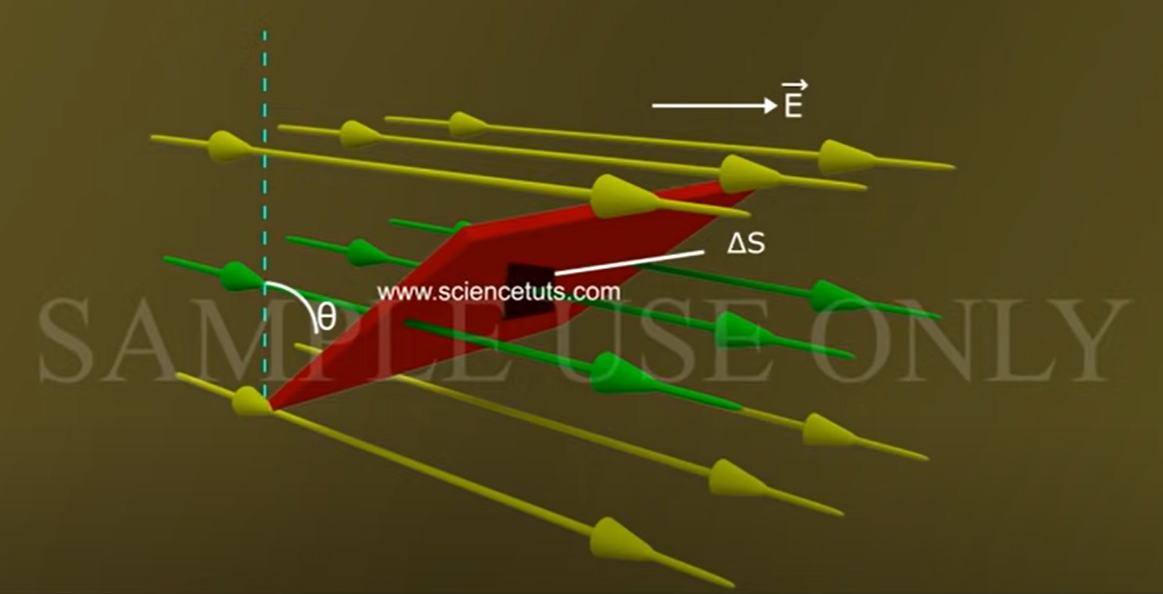
\includegraphics[scale=0.5]{SurfaceIntegralKind2.png}
\end{figure}
Мінус даної формули: вона застосовна лише для прямокутної площини. Ось тут виникає цей підрозділ.\\
А тепер нехай задана деяка поверхня $\Sigma$ - гладка, всюди неособлива та $\vec{r}$ - її параметризація в області $D$.\\
Як це було минулого разу, ми розіб'ємо поверхню, буде $\lambda_\Sigma$. А потім утворимо відмічені точки $N$. Там далі на кожній підповерхні буде прямокутна поверхня.\\
На відміченій точці $N_i$ поверхні проведемо дотичну $T^*_{N_i} \Sigma(v_1,v_2)$. Там є напруженність $\vec{E}(N_i)$ (для спрощення ми обмежимось лише неперервним векторним полем). А тому потік можна обчислити за формулою $( \vec{E}(N_i), \overrightarrow{T^*_{N_i} \Sigma(v_1,v_2)} )$.\\
Тоді визначається нова інтегральна сума, але тут це буде сума всіх робіт:
\begin{align*}
\sigma(\vec{F},\lambda,N) = \displaystyle\sum_{v_1,v_2} \left( \vec{E}(N_i), \overrightarrow{T^*_{N_i} \Sigma(v_1,v_2)} \right)
\end{align*}
У цьому випадку $\overrightarrow{T^*_{N_i} \Sigma(v_1,v_2)}$ - вектор площі даної дотичної.\\
Надалі я знову позначатиму векторне поле за $\vec{F}$, тому що так простіше.

\begin{definition}
Число $J$ називається \textbf{поверхневим інтегралом II роду} від векторного поля $\vec{F}$ вздовж поверхні $\Sigma$, якщо
\begin{align*}
\forall \varepsilon > 0: \exists \delta > 0: \forall (\lambda_\Sigma, N): |\lambda|_\Sigma < \delta \implies |\sigma(\vec{F},\lambda_\Sigma, N) - J| < \varepsilon
\end{align*}
Позначення: $J = \displaystyle\iint_\Sigma (\vec{F}, d\vec{S})$.
\end{definition}

\begin{remark}
Зокрема якщо векторне поле $\vec{F} = ( P(x,y,z), Q(x,y,z), R(x,y,z) )^T$, то тоді використовується інше позначення:\\
$\displaystyle\int_\Sigma P(x,y,z)\,dy\,dz + Q(x,y,z)\,dx\,dz + R(x,y,z)\,dx\,dy$.\\
Інтуїція даного позначення згодом.
\end{remark}

\begin{remark}
У разі якщо поверхня $\Sigma$ буде замкнутою, то прийнято позначти це таким чином: $\displaystyle\oiint_{\Sigma} (\vec{F}, \,d\vec{S})$.
\end{remark}

\begin{theorem}
Задано $\Sigma$ - гладка поверхня, всі точки неособливі та $\vec{r}: D \to \mathbb{R}^3$ - параметризація в замкненій області. Нехай векторне поле $\vec{F} = (P,Q,R)^T: \Sigma \to \mathbb{R}^3$ - неперервне на $\Sigma$. Тоді існує поверхневий інтеграл ІІ роду, причому\\
$\displaystyle\iint_\Sigma (\vec{F},d\vec{S}) = \iint_D \left(\vec{F}(\vec{r}(u,v)), [\vec{r}'_u, \vec{r}'_v]\right)\,du\,dv$.\\
\textit{Поки без доведення. Я щось заплутався.}
\end{theorem}

\iffalse
\begin{proof}
Спочатку зауважимо, що $\vec{n} = \dfrac{[\vec{r}'_u, \vec{r}'_v]}{\Norm{[\vec{r}'_u, \vec{r}'_v]}}$. А також треба побачити, що $\overrightarrow{T^*_{N_i} \Sigma(v_1,v_2)} = \vec{n} \cdot S(T^*_{N_i} \Sigma(v_1,v_2))$. Але ось ця площа - це фактично площа паралелограму, а це ж є норма векторного добутку. Таким чином,\\
$(\vec{F},\overrightarrow{T^*_{N_i} \Sigma(v_1,v_2)}) = (\vec{F}, [\vec{r}'_u, \vec{r}'_v ])$
\end{proof}
\fi

\begin{corollary}
$\displaystyle\iint_\Sigma (\vec{F}, d\vec{S}) = \iint_\Sigma (\vec{F}, \vec{n})\,dS$.
\end{corollary}

\begin{theorem}
Маємо $\vec{r_1},\vec{r_2}$ на відповідно $D_1, D_2$ - дві параметризації однієї й той самої поверхні. Тоді\\
$\displaystyle\iint_{\Sigma_1} (\vec{F}\,d\vec{S}) = \iint_{\Sigma_2} (\vec{F}\,d\vec{S})$, якщо ці поверхні однієї орієнтації;\\
$\displaystyle\iint_{\Sigma_1 } (\vec{F}\,d\vec{S}) = -\iint_{\Sigma_2} (\vec{F}\,d\vec{S})$, якщо ці поверхні різної орієнтації.\\
Тобто поверхневи інтеграл ІІ роду не залежить від параметризації, але має значення орієнтація поверхні.
\end{theorem}

Якщо стисло, то у нас вектори нормалі або напрямлені зовні, або всередині.

\subsection{Формула Остроградського-Гауса}
\begin{definition}
Задано $V \subset \mathbb{R}^3$ - область та векторне поле $\vec{F}: V \to \mathbb{R}^3$, де $\vec{F} = (P,Q,R)^T$ - неперервно-диференційовано на $V$.\\
\textbf{Дивергенцією} векторного поля $\vec{F}$ назвемо відображення $\text{div} \vec{F}: V \to \mathbb{R}$, що задається як
\begin{align*}
\text{div} \vec{F}(x,y,z) = \departial{P}{x}(x,y,z) + \departial{Q}{y}(x,y,z) + \departial{R}{z}(x,y,z)
\end{align*}
\end{definition}

\begin{lemma}
Задано множину $C$ - криволінійний циліндр (обмежується функціями $z(x,y)$). Нехай $\vec{F} = (P,Q,R)^T$ визначено на $C$ та неперервно-дифереційоване. Тоді, припустивши, що $\partial  C$ має зовнішню орієнтацію, маємо\\
$\displaystyle\oiint_{\partial C} R\,dx\,dy = \iiint_C \departial{R}{z}\,dx\,dy\,dz$.
\end{lemma}

\begin{proof}
Маємо $C = \{ (x,y) \in pr_{XOY}C: z_1(x,y) \leq z \leq z_2(x,y) \}$. Тоді:\\
$\displaystyle\iiint_C \departial{R}{z}\,dx\,dy\,dz = \iint_{pr_{XOY} C}\,dx\,dy \int_{z_1(x,y)}^{z_2(x,y)} \departial{R}{z}\,dz = \iint_{pr_{XOY} C} R(x,y,z_2(x,y)) - R(x,y,z_1(x,y))\,dx\,dy = \\
= \iint_{pr_{XOY} C} R(x,y,z_2(x,y))\,dx\,dy - \iint_{pr_{XOY} C} R(x,y,z_1(x,y))\,dx\,dy$.\\
Тепер розглянемо ліву частину рівності. Маємо:\\
$\displaystyle\oiint_{\partial C} R\,dx\,dy = \iint_{\partial C_1} R\,dx\,dy + \iint_{\partial C_2} R\,dx\,dy + \iint_{\partial C_{side}} R\,dx\,dy$.\\
Тут $\partial C_{side}$ - це бічна сторона. Бічна сторона паралельна $OZ$, а тому $\vec{n} \perp OZ$, власне звідси $\vec{n} = (n_1,n_2,0)$. Таким чином,\\
$\displaystyle\iint_{\partial C_{side}} R\,dx\,dy = \iint_{\partial C} ((0,0,R)^T, \vec{n})\,dx\,dy = 0$.\\
Тут $\partial C_1$ - це нижня основа. Проєктуємо його на $XOY$. Оскільки $C$ орієнтовна зовні, то туди кут між $OZ$ та $\vec{n}$ буде від'ємним, а тому \\
$\displaystyle\iint_{\partial C_1} R\,dx\,dy = -\iint_{pr_{XOY} C} R(x,y,z_1(x,y))\,dx\,dy$.\\
Тут $\partial C_2$ - це верхня основа, а всі решта міркування аналогічні, отже,\\
$\displaystyle\iint_{\partial C_2} R\,dx\,dy = \iint_{pr_{XOY} C} R(x,y,z_2(x,y))\,dx\,dy$.\\
Отже, остаточно отримали рівність $\displaystyle\oiint_{\partial C} R\,dx\,dy = \iiint_C \departial{R}{z}\,dx\,dy\,dz$.
\end{proof}

\begin{lemma}
Задано множину $V$ - замкнена область. Нехай $\vec{F} = (P,Q,R)^T$ визначено на $V$ та неперервно-диференційоване. Тоді, припустивши, що $\partial V$ має зовнішню орієнтацію, маємо\\
$\displaystyle\oiint_{\partial V} R\,dx\,dy = \iiint_V \departial{R}{z}\,dx\,dy\,dz$.
\end{lemma}

\begin{proof}
Ми розіб'ємо область на криволінійні циліндри, бічні сторони якись паралельні $OZ$, таким чином:\\
$V = \displaystyle\bigcup_{i=1}^n C_i$, причому вони не мають спільних внутрішніх точок. Тоді звідси\\
$\displaystyle\iiint_V \departial{R}{z}\,dx\,dy\,dz = \sum_{i=1}^n \iiint_{C_i} \departial{R}{z}\,dx\,dy\,dz$.\\
А з іншого боку, $\displaystyle\sum_{i=1}^n \iiint_{C_i} \departial{R}{z}\,dx\,dy\,dz = \sum_{i=1}^n\oiint_{\partial C_i} R\,dx\,dy$.\\
Тут варто зауважити, що $\partial C_i = (\partial V \cap \partial C_i) \cup \displaystyle\bigcup_{\substack{k = 1 \\ k \neq j}}^n (\partial C_i \cap \partial C_k)$. Аналогічно, як в Гріна, але уявити дуже важко.\\
Абсолютно аналогічно, як в Гріна, ми розпишемо\\
$\displaystyle\sum_{i=1}^n\oiint_{\partial C_i} R\,dx\,dy = \sum_{i=1}^n \left( \iint_{\partial V \cap \partial C_i}R\,dx\,dy + \sum_{\substack{k = 1 \\ k \neq j}}^n \iint_{\partial C_i \cap \partial C_k}R\,dx\,dy \right)$.\\
Тепер окремо розглянемо $\displaystyle\sum_{i=1}^n \sum_{\substack{k=1 \\ k \neq j}}^n \iint_{\partial C_i \cap \partial C_k} R\,dx\,dy$. У цій сумі беруть участь одночасно $\displaystyle\iint_{C_{i_0} \cap C_{k_0}} R\,dx\,dy$ та $\displaystyle\iint_{\partial C_{k_0} \cap \partial C_{i_0}} R\,dx\,dy$ при $i_0 \neq k_0$, а також $1 \leq i_0,k_0 \leq n$. У цих двох поверхнось під інтегралами орієнтації протилежні один одному, якщо придивитись на 3D малюнок (що дуже важко намалювати), а тому звідси\\
$\displaystyle\iint_{\partial C_{i_0} \cap \partial C_{k_0}} R\,dx\,dy + \iint_{\partial C_{k_0} \cap \partial C_{i_0}} R\,dx\,dy = 0$.\\
Звідси випливає, що $\displaystyle\sum_{i=1}^n \sum_{\substack{k=1 \\ k \neq j}}^n \iint_{\partial C_i \cap \partial C_k} R\,dx\,dy = 0$, а тому продовжимо рівність:\\
$\displaystyle\sum_{i=1}^n \oiint_{\partial C_i} R\,dx\,dy = \sum_{i=1}^n \iint_{\partial V \cap \partial C_i} R\,dx\,dy = \oiint_{\partial V} R\,dx\,dy$.\\
Дійсно, $\displaystyle\bigcup_{i=1}^n (\partial V \cap \partial C_i) = \partial V$, як об'єднання всіх меж.\\
Разом отримали, що $\displaystyle\oiint_{\partial V}R\,dx\,dy = \iiint_V \departial{R}{z}\,dx\,dy\,dz$.
\end{proof}

Абсолютно аналогічно можна довести ці дві леми для випадку:\\
$\displaystyle\oiint_{\partial V}Q\,dx\,dz = \iiint_V \departial{Q}{y}\,dx\,dy\,dz$\\
$\displaystyle\oiint_{\partial V}P\,dy\,dz = \iiint_V \departial{P}{x}\,dx\,dy\,dz$.\\
Тільки в першому треба проєкцію на $OXZ$, а другому треба проєкцію на $YOZ$. І криволінійні циліндри будуть по функціям відповідно $x_1(y,z),x_2(y,z)$ та $y_1(x,z), y_2(x,z)$. Разом отримаємо результат:

\begin{theorem}[Теорема Гауса-Остроградського]
Задано $V \subset \mathbb{R}^3$ - замкнена область та $\partial V$ - границя, що орієнтовна зовні. Відомо, що $\vec{F} = (P,Q,R)^T$ визначено на $V$ та неперервно-диференційовано. Тоді\\
$\displaystyle\iint_{\partial V} P\,dy\,dz + Q\,dx\,dz + R\,dx\,dy = \iiint\displaylimits_V \text{div} \vec{F}\,dx\,dy\,dz$. 
\end{theorem}

\subsection{Формула Стокса}
\begin{definition}
Задано $V \subset \mathbb{R}^3$ - область та векторне поле $\vec{F}: V \to \mathbb{R}^3$, де $\vec{F} = (P,Q,R)^T$ - неперервно-диференційовано на $V$.\\
\textbf{Ротором (вихром)} векторного поля $\vec{F}$ назвемо відображення $\text{rot}\vec{F}: V \to \mathbb{R}^3$, що задається як
\begin{align*}
\text{rot} \vec{F}(x,y,z) = \det \begin{pmatrix}
\vec{i} & \vec{j} & \vec{k} \\
\departial{}{x} & \departial{}{y} & \departial{}{z} \\
P & Q & R
\end{pmatrix} (x,y,z)
\end{align*}
\end{definition}

\begin{definition}
Поверхню $\Sigma$ та криву $\partial \Sigma$ назвемо \textbf{узгоджено напрямленими}, якщо обхід $\partial \sigma$ відбувається проти годинникової стрілки під час спостереження з кінця вектора $\vec{n}$.
\end{definition}

\begin{theorem}[Теорема Стокса]
Задано $U \subset \mathbb{R}^3$ - відкрита множина та $\sigma \subset U$ - гладка поверхня так, що $\sigma = \Gamma_f = \Gamma_g = \Gamma_h$ для функцій $f,g,h$ на $D_{yz},D_{zx},D_{xy}$.\\
Нехай $\partial \sigma$ - границя поверхні $\sigma$ та $\vec{F} = (P,Q,T)^T$ визначено на $U$ та неперервно-диференційовано. Тоді, припустивши, що $\partial \sigma$ узгоджено орієнтована з $\sigma$, маємо\\
$\displaystyle\oint_{\partial \sigma} (\vec{F}, d \vec{l}) = \iint_\sigma (\text{rot} \vec{F}, \vec{n})\,d\sigma$.
\end{theorem}

\begin{proof}
Спочатку доведемо частинний випадок - і це буде $\displaystyle\int_{\partial \sigma} P\,dx = \iint_\sigma \departial{P}{z}\,dx\,dz - \departial{P}{y}\,dx\,dy$.\\
Дуже хочеться застосувати формулу Гріна, але поки що крива задається не на площині, а в просторі, треба виправити цю ситуацію.
\end{proof}

\subsection{Незалежність криволінійного інтегралу ІІ роду від шляху інтегрування в $\mathbb{R}^3$}
\begin{lemma}[Лема Пуанкаре в $\mathbb{R}^3$]
Задано множину $V \subset \mathbb{R}^3$ - замкнена однозв'язна область. Нехай $\vec{F} = (P,Q)^T$ визначено на $V$ та неперервно-диференційоване. Тоді нижчезгадані твердження еквівалентні:\\
1. $\departial{R}{y}(x,y,z) = \departial{Q}{z}(x,y,z); \departial{R}{x}(x,y,z) = \departial{P}{z}(x,y,z); \departial{Q}{x}(x,y,z) = \departial{P}{x}(x,y,z), \forall (x,y,z) \in V$.\\
Або, що еквівалентно, $\text{rot} \vec{F} = \vec{0}$;\\
2. $\displaystyle\oint_{\Gamma} P(x,y)\,dx + Q(x,y)\,dy = 0$ для будь-якої замкненої кривої $\Gamma \subset V$.\\
3. $\displaystyle\int_{\Gamma_1} P\,dx + Q\,dy = \int_{\Gamma_2} P\,dx + Q\,dy$ для будь-яких двох кривих $\Gamma_1, \Gamma_2 \subset V$ зі спільним початком та кінцем;\\
4. Існує $U(x,y,z)$ - двічі неперервно-дифереційована функція, для якого $\departial{U}{x}(x,y,z) = P(x,y,z)$, $\departial{U}{y}(x,y,z) = Q(x,y,z)$, $\departial{U}{z}(x,y,z) = R(x,y,z), \forall (x,y,z) \in V$. Інакше кажучи,\\ $dU(x,y) =  P(x,y)\,dx + Q(x,y)\,dy$.\\
\textit{Доведення повторюється, тому нема сенсу розписувати.}
\end{lemma}
\end{document}